% $Author: predrag $ $Date: 2018-12-07 13:04:16 -0500 (Fri, 07 Dec 2018) $

%\svnkwsave{$RepoFile: elton/blog/adjoint.tex $}
%\svnidlong {$HeadURL: svn://zero.physics.gatech.edu/elton/blog/adjoint.tex $}
%{$LastChangedDate: 2018-12-07 13:04:16 -0500 (Fri, 07 Dec 2018) $}
%{$LastChangedRevision: 547 $} {$LastChangedBy: predrag $}
%\svnid{$Id: adjoint.tex 547 2018-12-07 18:04:16Z predrag $}


\chapter{Bloggin' adjoint paper}
\label{chap:blogAdjoint}

\begin{bartlett}
\bauthor{311}
All mixed up, you don't know what to do \\
Next thing you turn around and find the person is you
\end{bartlett}
%
%\vspace{0.2in}
%
%$\footnotemark\footnotetext{{\tt \svnkw{RepoFile}}, rev. \svnfilerev:
% last edit by \svnFullAuthor{\svnfileauthor},
% \svnfilemonth/\svnfileday/\svnfileyear}$
%\bigskip
%


\noindent
{\color{red} The latest entry at the top for this blog}
\bigskip\bigskip

\section{Daily blog}
\label{sect:DailyBlog}
\begin{description}
\MMFpost{2015-08-24}{Response to Predrag's comments:
\begin{enumerate}
\item
Predrag: Place someplace on the web (Openpipe flow? ChaosBook?) snapshots of
all your solutions - I already miss them, to check their symmetries -
their symmetries etc., and the data files so other people can check
them / use them. You probably have most of them plotted in the blog,
but in blog figures they are unlabelled, and without value of $I$,
so it is impossible to tell who is who.

\item
Predrag: Why not $c(0)=0.01$? When you know that is a typical number.

\item
Predrag: Does not matter how many flies sit on them, $(I,D)$ plots are stupid. If you must plot
them, immediately define $I$ and $D$ to be normalized, so you do not have to write
$I/I_{lam}$ over and over again. Plot $(I,I-D)$ - that is better use of paper than having
everything stick to the diagonal, with large off-diagonal white regions, and
$\dot E = I-D$ so it is a perfectly legal quantity to plot.

\item
Predrag: I would bet that no (relative) equilibria belong to the inertial manifold: they are
either isolated or have vanishingly small PDF in their neighborhoods.

Mohammad:

%\item
%Predrag: No, no, by symmetry you can vary only the relative phase, so only one
%$\ell_1$ matters. I got rid of your
%$\|\mathcal T_{\ell_1}g_1\vc u^1-\mathcal T_{\ell_2}g_2\vc u^2\|_{L^2}$.

\item
Predrag: You sure about that? $I[\vc u]$ is linear
in $\vc u$ means $I[\vc u]=K\vc u + \vc \ell$. Why should the matrix $K$ commute
with matrix $\mathcal P$? At most, it can be decomposed into sum over irreps.
If I am right,
$I[\vc u-\mathcal P\vc u] \neq 0$.

\item
Predrag: Fig.~\ref{fig:Pw_erg}: The fundamental tile tiles
the square (I would prefer a rectangle, with different $L_1,\;L_2$).
Nothing is gained by plotting its 16 copies.

\item Predrag 2015-08-23:
    I would follow Sirovich\rf{Sirovich87} and call this
    `glide reflection' throughout, a well established term (see the blog),
    not yet another confusing `shift-reflect'. Unless you have authority
    earlier than Sirovich to cite.

\item Predrag 2015-08-21:
    Though plumbers do not get it, you do not have to continuously rotate anything:
    our slice\rf{FrCv11} is \emph{defined} as the minimal distance condition. You just
    have to make sure that is a global, not local minimum.

\item Predrag 2015-08-21:
    In no sense is $\vc u-\mathcal P\vc u$ ``anti-symmetric'' - this decomposes into
    a number of irreps which I have counted (or neglected to count) in the blog.

\item Predrag 2015-08-20
    Include someplace 2D configuration space snapshots of a turbulent state:
    perhaps add 6 panels that show the not-symmetrized vorticity $\omega$ at the same instants
    as panels of Figure~\ref{fig:Pw_erg}.

\item Predrag 2015-08-23
IDiocy continued: why are $I\simeq D$ in 4 out of 6 snapshots in Fig.~\ref{fig:Pw_erg},
and all are in the `ergodic swamp'?
Probably does not matter, but perhaps far away from diagonal or at higer
dissipation rates the shapes are more interesting...

\end{enumerate}
}
\MMFpost{2015-08-24}{To do list for the 2nd paper:
\begin{enumerate}

\item Predrag 2015-08-21:
\eqref{KFeqv0} suggests a solution amplitude cares about $Re$ and the
wave number, so initial guesses could be crafted with amplitude,
energy, dissipation rate etc. closer to states on the attractor.
Something like this has 40 times larger amplitude, perhaps, while retaining the
symmetry:
$$
\vc u_0^{(m_1,m_2)}=
\big(\frac{Re}{m_2^2}\sin(m_2x_2),\frac{Re}{m_1^2}\sin(m_1x_1)\big)
$$

\item Predrag 2015-08-21:
    Fig.~\ref{fig:EQ_diag} is not helpful; the ordering of initial
    guesses is not good. Initial guesses should be classified by their
    symmetries (subgroups of $D_{16}$), and so should the \eqva\ reached
    - as far as I remember, the hybrid method stayed within the invariant
    subspace. In reordered plot, you will have diconnected blocks. Also
    solutions related by discrete symmetries should be counted only once
    - I assume you do that? Put all that in
    the 2nd paper?

\item
That is why in the pipe paper we report the Kaplan-Yorke dimension -
have you tried that? Also, if the leading eigenexponent is complex,
you have to take $2\mu_1$, not $\mu_1$. So the $E_8$ number is
$2\mu_1=2 \times 0.61189$, and this is not a good example.

\item
In \eqref{DnA1proj} you define ${\mathcal P}_{A1}$ of $D_n$ (see my blog notes).
This is one of the coordinates of state space projections of
\rf{GHCW07}. Now that you are using their visualization anyway, in 1 dim,
it costs you
nothing to also look at another cheap coordinate, the anti-symmetric 1-dimensional irrep $A2$
projection,
\(
{\mathcal P}_{A2} = \frac{1}{4n}\sum_{m=0}^{2n-1}\mathcal S^m\left(1 -\mathcal R\right)
\,.
\).
This way you can visualize visits to $E_{13}$ in a plane, rather than as a time
series Fig.~\ref{fig:distE13}.

\item Predrag 2015-08-23
    Delineate the fundamental tile $[-1/2,1/2]\times[0,1/8]$ in
    Fig.~\ref{fig:Pw_erg}\,(f), and indicate the action of discrete
    symmetry operations $\mathcal R$ and $\mathcal S$ on it. Say it tiles
    the square (I would prefer a rectangle, with different $L_1,\;L_2$).
    From then on, you can plot only the fundamental tile, nothing is gained by
    plotting its 16 copies.

\item Predrag 2015-08-23
    I am guessing that symmetry group of $E_{13}$ is $D_1 \times D_1$, order 4, so there
    are 4 distinct copies of it on the unit square domain, and there are 4 distinct
    shortest heteroclinic connections from `here' to $E_{13}$. One might look at the least
    contracting eigenvectors of $E_{13}$ and their symmetries, to see whether one can get
    to it. It is not an obvious candidate for the cause of `intermittency' - it has 16 unstable
    directions...

\end{enumerate}
}

\PCpost{2015-08-22}{
I have scanned through the wikis, and to me the adjoint descent looks
different, but I am not sure. In the same spirit, the
\HREF{https://en.wikipedia.org/wiki/Biconjugate_gradient_stabilized_method}
{biconjugate gradient stabilized method} looks like a close relative.
            }

\item[2015-08-22 Andre Souza] sandre@umich.edu (Predrag has asked him to
have look at the adjoint.tex manuscript, as he is using a variety of
optimization codes in control theory):
This looks to me like the biconjugate gradient version of
\HREF{https://en.wikipedia.org/wiki/Nonlinear_conjugate_gradient_method}
{nonlinear conjugate gradient method},
which corresponds to using conjugate gradient on the normal equations.

Said differently, it seems to be the nonlinear analog of
\HREF{https://en.wikipedia.org/wiki/Biconjugate_gradient_method}
{biconjugate gradient method}.

A preconditioner ($\mathcal{A}$ in the manuscript) similar to an
inverse Laplacian is generally a good one for stability and convergence
in low Reynolds number scenarios. Although in my experience such a
precondition will probably not work too well for high Reynolds numbers
where the nonlinear term is most important.

There are papers that I have read that attempt to find fixed points or
periodic solutions to PDEs by considering them as an optimal control
problem with an appropriately chosen functional. It may turn out that
Farazmand's algorithm is fundamentally different (due to my cavalier
reading of the document), but it does seem similar.

\PCpost{2015-08-19}{
Morally length is a length, so I do not think of $L_i$ as
non-dimensional. In any case, you should be able to go back to
dimensional units, and how is `1' going to become `$L^{-2}$'? so
\refeq{eq:H-1_foias} suits me best. Except it should be $(2\pi)^2$. Are
you sure that averages (0$th$ Fourier modes) do not vanish in your
application? If they do, there is no need for the pesky `1' or $L^{-2}$
term in the denominator, you can define the homogenous $H^{-1}$ norm as
\begin{align}
  \norm{ \mu }^{2}_{2,-s} := \sum_{k\neq 0}
  \frac{ \left\lvert{\hat \mu(k)}\right\rvert^{2} }{{k}^{2s}}
\,.
\label{eq:neg-sob-norm0}
\end{align}
Saying ``they are all mathematically {equivalent}" is OK when proving
theorems, but inconvenient when computing: $10^{-12}+|2\pi\mathbf
k/\mathbf L|^2$ and $1+|2\pi\mathbf k/\mathbf L|^2$ might be
``mathematically {equivalent}", but they might give you quite different
``distances''. It would be nice to have a natural choice of the constant
term, motivated by one elementary example, where one can see that `1' or
`$(2\pi)^2$' is the natural choice.

But you are right. Literature defines ``Japanese bracket"
$\langle x \rangle :=
(1+|x|^2)^{1/2}$ because that is a smooth function, while $|x|$ is not differentiable
at $x=0$; then smooth out gradients by
$\langle \nabla \rangle = (1+ \nabla^2)^{1/2}$.
 On the real line $x\in\reals$ unit length `1' is as good as anything. On a
periodic domain $L$ I would guess on needs to define something like
analytic periodic norm
$\langle x \rangle := L(\cos(2\pi x/L)^{1/2})$. However, that is not how they define it -
see \HREF{http://texas.math.ttu.edu/~gilliam/f06/m5340_f06/sobolev_sp_circle.pdf}
{Gilliam's notes}, where it is done for the circle $x\in[0,2\pi]$, and immediately defined in the Fourier space,
no mention of Laplacians. I should also work it out for a finite periodic lattice - that's
what we compute on.
    }

\MMFpost{2015-07-30}{To Predrag: You made a very good point about the $H^{-1}$ norm. I have seen
different textbooks using different scalings for the $|\mathbf k|^2$ term, but never
paid much attention to it. So, I reviewed the definitions and here are a few subsequent comments.
\begin{itemize}
\item You observe that ``Number `1' in the denominator in \refeq{eq:Afs}
makes no sense, as the dimension of your $|\vc k|^2$ is $L^{-2}$."
Note that the Navier--Stokes equation in the paper is assumed to be in
non-dimensional variables. So, $L_i$ are non-dimensional lengths.
So I guess there is no dimensional inconsistency, is there?

\item The definition of $H^{-1}$ norm used in\rf{BudMez12} actually coincides with
mine as they scale their domain-size to be unity, i.e., they work on the torus
$\mathbb T^2=[0,1]^2$. They are more explicit about the domain size here\rf{MathMez07}.

\item In fact,\rf{foias2001} is the only reference I could find which uses a $H^{-1}$ definition
that is consistent even when the lengths $L_i$ are dimensional. Let $\mathbf k/\mathbf
L=(k_1/L_1,k_2/L_2,k_3/L_3)$.
Instead of $1+|2\pi\mathbf k/\mathbf L|^2$ (the term I use in the paper),\rf{foias2001}
(cf. Eq. (5.26)) use
\beq
L^{-2}+2\pi|\mathbf k/\mathbf L|^2,
\label{eq:H-1_foias}
\eeq
where $L$ is one of the box lengths.

I do not understand why $2\pi$ is not squared, but at any rate, their definition is dimensionally
consistent.

\item Terry Tao points out in his
\href{https://terrytao.wordpress.com/2009/04/30/245c-notes-4-sobolev-spaces/}{blog} that

``Now observe that the quantity $\sum_{j=0}^k (2\pi |\xi|)^{2j}$ is comparable (up to constants
depending on $k,d$) to the expression $\langle \xi \rangle^{2k}$, where $\langle x \rangle :=
(1+|x|^2)^{1/2}$ (this quantity is sometimes known as the ``Japanese bracket" of $x$)."

Based on this, he goes on to replace $2\pi |\xi|$ with $|\xi|$ in his
definition of the Sobolev norms.
\end{itemize}

To summarize, as you observe, only~\eqref{eq:H-1_foias} is physically meaningful when
the lengths $L_i$ are dimensional. When non-dimensionalized, they are all
mathematically \emph{equivalent}, in the technical sense of the word.

In the context of the paper, all that matters is that $\mathcal A$ is a self-adjoint,
positive-definite operator that damps higher Fourier mode. It is an afterthought that
my choice of $\mathcal A$ renders the norm as $H^{-1}$.
}

\PCpost{2015-07-19, 2015-07-28}{This keeps bugging me in your draft:
``Let $\vc q=(\vc u,p)$ be the
velocity-pressure pair and define
the operator $\mathcal A$ through its action in
the Fourier space,
\beq
\widehat{\mathcal A\vc q}(\vc k) = \frac{\widehat{\vc q}(\vc k)}{1+|\vc k|^2},
\label{eq:Afs}
\eeq
where $\widehat{\vc q}$ denotes the Fourier transform of $\vc q$ and $\vc
k=(2\pi k_1/L_1,2\pi k_2/L_2,2\pi k_3/L_3)$, with $k_i\in\mathbb Z$ being the
wavenumber.''

In our papers we define
${\bf q_k}=(2\pi k_1/L_1,2\pi k_2/L_2,2\pi k_3/L_3)$,
while the components of $\vc k$ are the usual
$\vc k=(k_1,k_2,k_3).$ Number ``1'' in the denominator in \refeq{eq:Afs}
makes no sense, as the dimension of your $|\vc k|^2$ is $L^{-2}$.

Budi\v{s}i\'c and Mezi\'c\rf{BudMez12} are big fans of Sobolev, too.
Their definitions make more sense to me:

[...] the Sobolev space \(W^{2,-s}\), whose norm can be defined as a weighted euclidean norm
\begin{align}
  \norm{ \mu }^{2}_{2,-s} := \sum_{k \in \mathbb{Z}^{D}}
  \frac{ \left\lvert{\hat \mu(k)}\right\rvert^{2} }
  {\left[1 + (2k\pi)^{2} \right]^{s}}
,\label{eq:neg-sob-norm}
\end{align}
with the index determined as \(s = (D+1)/2\) where \(D = \dim M\). We use
\(\ell^{2,-s}\) as the symbol for the associated Fourier coefficient
space with the weighted euclidean norm. An excellent introduction to the
Sobolev space theory is the classic textbook by Adams\rf{Adams:2003wi},
which contains all the material relevant for this
analysis.

}



\MMFpost{2015-07-20}{Predrag, thanks for your careful reading of the manuscript.
I responded to your comments so far. Please see the paragraphs starting with
``{\bf Mohammad:}", below.
}

\PCpost{2015-07-23}{ Regarding your sentence:
``The idea that turbulent fluid flow can be studied in terms of
the invariant solutions of Navier--Stokes equations dates back to
1940s~\rf{landau44,hopf48}.''

I would be very happy if you could show me where the idea is in the
Landau paper\rf{landau44}. It is certainly not Hopf\rf{hopf48} - I
discuss that in the ChaosBook history appendix, turbulence section. As
far as I know, it is first stated explicitly end demonstrated for
chaos/turbulence in a PDE, in our \refref{Christiansen:97}. If you find
an earlier reference, let me know.

I personally cite Hopf\rf{hopf48} because it is a key paper in
the history of turbulence - he emphasizes the necessity of working in
\statesp\ (phase space) and the importance of natural measure.
He is a dead white male - if I
cited myself, everybody would complain, but nobody has problems with Hopf.
A very pleasant read is
\HREF{http://webusers.imj-prg.fr/~david.aubin/These/chap7-1.pdf}
{David Aubin}'s French perspective on the modern theory of turbulence.

{\bf Mohammad:} Well, you caught me there! I didn't personally read
the original papers of Hopf and Landau. I read later articles/books
that attribute the idea to these guys. Landau's work, for instance,
is referred to in \refref{Holmes96}. For Hopf, is it more appropriate
to cite Hopf 1942?

{\bf Predrag:} Hopf 1942 ``Abzweigung einer periodischen
L\"osung''\rf{hopf42}, nothing to do with invariant solutions. The paper
is commented in detail
\HREF{https://books.google.com/books?id=8TOqgRLbpaQC} {here} by
Golubitsky and Rabinowitz. If you get the book, check out Peter Lax
commentary - that also looks very interesting.
Kielh\"ofer\rf{Kielhofer79} discussion of Hopf bifurcations looks nice.
\HREF{http://www.ucl.ac.uk/~ucesgvd/hopf.pdf} {Gert van der Heijden}
discusses the Hopf bifurcation for flows, Hopf bifurcation for maps (or
Neimark-Sacker bifurcation) and the Hamiltonian-Hopf bifurcation.

Landau\rf{landau44} and Hopf\rf{hopf48} papers are always referenced for
their (wrong)
\HREF{https://en.wikipedia.org/wiki/Landau\%E2\%80\%93Hopf_theory_of_turbulence}
{theory of turbulence}, as a linear sum of infinity of incommensurate
Fourier modes. I believe you can find the English translation
reprinted in Hao (1984), in the CNS library in my office.
In other words, Hopf and Landau have nothing to do with
the idea at hand. The earliest paper I can track down that talks about
periodic orbits in turbulence is
1966 Spiegel and Moore paper\rf{MS66}.

Tell me where in \refref{Holmes96} are Landau and Hopf credited for ``The
idea that turbulent fluid flow can be studied in terms of the invariant
solutions of Navier--Stokes equations''? What I know is described in
ChaosBook.org appendix \emph{A.5 Dynamicist's vision of turbulence}.
    }

\PCpost{2015-07-19}{
Have a quick look at Nagata's papers\rf{N90,N97} - what I remember of
his approach is that was analytic continuation of Couette-Taylor
solutions to plane Couette.

{\bf Mohammad:} Double checked. Nagata does formulate a large
algebraic system and then use Newton to find its solutions:
``Having obtained TVF solutions by a Galerkin method and a Newton-Raphson
method for the truncated system of nonlinear algebraic equations for $a_{ln}$, $b_{ln}$ and
$c_k$..."
}

\PCpost{2015-07-19}{
My recollection is that we\rf{GHCW07} in 2006 were first to use ``close
recurrences of a turbulent trajectory'' for Navier-Stokes, not
\refrefs{DV04,kawahara06}. Ask Gibson. The close recurrences method was
introduced in \refref{pchaot}, in 1987.

{\bf Mohammad:} \refRef{kawahara06} uses recurrences. They write:
``In a weakly turbulent state at relatively low Reynolds number
$Re_\lambda=57$ we search for a recurrent state to be used as an initial
guess for the Newton-Raphson iteration..." \refRef{DV04} also uses
recurrences; see Section 2.1. \refRef{GHCW07} is actually published in
2008, but needs to be cited regardless. I added the citation. For
\refref{pchaot}, I am sorry, I was ignorant of this publication. It is
now cited in the manuscript.
\\
{\bf Predrag:}
Eckmann \etal\rf{EKR87} are credited for introducing the method of
recurrence plots, submission date June 1987. Procaccia wrote our
\refref{pchaot} which uses the method, submitted it March 1987. Ergo, we
are first.

Looking at gibson blog on svn - we were using recurrence plots for Navier-Stokes
since 2005, but we never published a paper on our periodic orbits
because John would not do it - I only wrote a short conference proceedings
about them\rf{CviGib10} where I cite only \refref{pchaot}.
\refRef{DV04} is about the Lorenz attractor, has no
Section 2.1 and one does not need recurrence plots for the problem at hand.
You mean Section 2.1 of \refref{Visw06}. That is an important paper,
done in interaction with Gibson and myself, but he was faster. Divakar
writes ``Our method has three new
aspects. Firstly, we describe a way to find good initial guess
es. Secondly, we show how to set up
the Newton equations for finding relative periodic solutions. Thirdly, we show how to modify the
Newton-Krylov procedure to compute the locally constrained optimal hook step.''
We always cite him for the last two - clearly, he deserves a citation for the first
aspect as well.
        }

\PCpost{2015-07-19}{
Why `Hilbert function space $\mathcal H$'? Is there a self-adjoint operator
anywhere? You probably require more smoothness than L2 - perhaps it is a
Banach space?
{\bf Mohammad:} A Hilbert space is a simply a space on which an inner product is
defined. It is independent of any operator. Over a Hilbert space the adjoint of operators
(whether they are self-adjoint or not) is defined unambiguously.
We clearly need more smoothness than $L^2$, but those smooth functions are a subset of
the $L^2$ space.

Lan and Cvitanovi\'c introduced continuous fictitious-time Newton
descent \refref{CvitLanCrete02,lanVar1} as a flow minimizing $\|\vc F
(\vc u)\|^2_{L^2}$, required
\[
\pmb{\mathcal L}(\vc u;\vc G(\vc u))=-\vc F(\vc u),
%\label{eq:G_newton_inf}
\]
 and applied them to 1D \KSe\ PDE. I am not aware of
any earlier references - I actually cooked up the name `Newton descent'.
You feel it is not the same method because we wrote it in terms of
G\"{a}lerkin truncation components rather than the G\^ateaux
derivative?

{\bf Mohammad:} I agree and cite \refref{CvitLanCrete02,lanVar1} now in the manuscript. However, as
far as I can tell,
you look for periodic orbits, where the explicit form of $\bf F$ is not known.

``In other words, the continuous fictitious-time
Newton method converges to an equilibrium solution of~\eqref{eq:pde} for
almost all initial conditions.'' and
``The above discrete iterations do not guarantee the global
convergence that the continuous fictitious-time Newton descent does.''
sounds wrong - at least half of the time
and (lacking a precise initial guess) maybe most of the time Newton descent
hungs up at some local minimum and never reaches zero?

{\bf Mohammad:} As long as the linear system
\[
\pmb{\mathcal L}(\vc u;\vc G(\vc u))=-\vc F(\vc u),
%\label{eq:G_newton_inf}
\]
has a solution, the continuous-time Newton descent cannot hung up in a local minimum. This is due
to the exact identity $\|\vc F(\vc u(\tau))\|_{L^2}=\|\vc F(\vc u(0))\|_{L^2}\exp(-\tau)$.
The linear system fails to have a solution when the linear operator $\pmb{\mathcal L}$
is singular, which is a co-dimension-one condition and does not occur generically.
That is why I used the term ``\emph{almost all initial conditions}" to be cautious.


I find $\dot H^{-1}$ awkward - hard not to think of the dot as a time derivative.
If it is a standard notation, refer to where you got it from, otherwise
maybe cook up something else?

{\bf Mohammad:} $\dot H^{-1}$ is standard notation
and is slightly
different from $H^{-1}$. But many authors simply use $H^{-1}$
in place of $\dot H^{-1}$ when the definition is explicated (as is in the manuscript).
So I could use $H^{-1}$ but then risk getting grilled by a pedantic referee.

You use $\mathcal H$' both for Hilbert function space (standard) and your
pace of divergence-free vector fields in $\dot H^{-1}$ (non-standard?).

{\bf Mohammad:} The $\dot H^{-1}$ happens to be a Hilbert function space.

``We found empirically, however, that the resulting equations are stiff'':
Is this really the reason? Or is it that you work in strong dissipation range,
with higher Fourier coefficients strongly suppressed?

{\bf Mohammad:} I found them stiff as a usual numerical integrator (RK) requires very small time
steps. \rf{yang07} observe the same for their system.

I find $\vc u''$ notation for $\vc F_{\vc 0}(\vc u)$ confusing,
because it makes $\vc u''$ appear to be related to
$\vc u$, which it definitely is not - it has a different dimension.
Desperately complex :)

{\bf Mohammad:} I agree that the notation might be confusing. The reason I don't use
$\vc F_{\vc 0}(\vc u)$ instead of $\vc u''$
is that the adjoint equation also has a pressure-type term
$p''$. Inspecting the derivation of the adjoint, you will see that $p''$ is the tween of $\vc u''$.
The notation $(\vc u'',p'')$ comes to me naturally through the definition/derivation of the
adjoint, but I'm open to better suggestions.
}

\MMFpost{2015-07-17}{To Predrag: I finalized a first draft that I am happy with.
Could you please read/edit/comment on this draft at your convenience?

Please note that I left out some of the material: reducing discrete symmetry, Poincar\'e map,
state space visualization. Those, in my opinion, could be a paper by themselves.
}

\PCpost{2015-07-06}{
I'm sorry my notes are such a mess. But yes, it is crucial that rotation
through $\pi$ and glide reflection do not commute, that is why the
symmetry (after continuous symmetry reduction) is $\Dn{8}$, see
\refeq{D8gen}.
    }

\PCpost{2015-07-06}{
`Intermittency' is a loaded word in the world of plumbing. I would be
reluctant to use it. Setting here is standard nonlinear dynamics: what
you mean is that there are rapid transitions between local repellers, or
`defects' in the language of pattern formation. We should recheck the
literature.
\\
{\bf Mohammad 2015-07-07:} Intermittency is a quite standard
term in fluid dynamics community. I see tons of papers on it
published regularly by plumbers, although they do not have the
dynamical systems perspective I present in the draft.
}

\PCpost{2015-07-07}{For standard notation on principal value, the
\HREF{https://en.wikipedia.org/wiki/Principal_value}
{wiki seems useful}.
    }

\MMFpost{2015-06-24}{
Do formulas \refeq{globalUBframe} still work?
\\
{\bf 2015-07-07} Now we need sum over 16 elements, otherwise the same.
Why don't you give it a try, replot \reffig{fig:proj_E4E7T2} in the
(correctly doubled number of elements) projection \refeq{globalUBframe}.
Naive version should produce 16 copies of fundamental domain. The one
reduced to the fundamental domain using your principal value argument should
put it all of the flow into one domain. Curious what going back to $2D$
plumber's visualization from fundamental domain gets us.
}


\MMFpost{2015-07-01}{Although, $\mathcal S$ and $\mathcal R$ do not commute, we still
have the following desirable equality
$$\sum_{m=0}^{2n-1}\left[\mathcal S^m\omega +\mathcal S^m\mathcal R\omega\right]=
\sum_{m=0}^{2n-1}\left[\mathcal S^m\omega +\mathcal R\mathcal S^m\omega\right].$$
This follows from the fact that $\mathcal R\omega=\mathcal S\mathcal R\mathcal S\omega$
and that the glide reflection is cyclic, i.e., $\mathcal S^{-1}=\mathcal S^{2n-1}$.
}

\MMFpost{2015-07-01}{Rotation through $\pi$, $\mathcal R$, and glide reflection $\mathcal S$
do NOT commute:
The action of $\mathcal R\mathcal S$ on the vorticity field is not equal
to the action of $\mathcal S\mathcal R$. We have
$$(\mathcal S\mathcal R\omega) (x_1,x_2)=-\omega\left(x_1,-x_2+\frac{\pi}{n}\right),$$
and
$$(\mathcal R\mathcal S\omega) (x_1,x_2)=-\omega\left(x_1,-x_2-\frac{\pi}{n}\right).$$
Therefore, $\mathcal R\mathcal S\neq \mathcal S\mathcal R$. From the above equations, we have
$\mathcal S^2\mathcal R\mathcal S\omega= \mathcal S\mathcal R\omega$ or equivalently
$$\mathcal R\omega=\mathcal S\mathcal R\mathcal S\omega.$$
}

\MMFpost{2015-07-01}{Reducing the discrete symmetries:
The action of the discrete symmetry $\mathcal S^m$ on the Fourier mode $(0,1)$ is
\beq
\widehat{\omega}(0,1)\mapsto(-1)^m\widehat{\omega}(0,1)e^{i\frac{m\pi}{n}}=
|\widehat{\omega}(0,1)|e^{i[\phi(0,1)+m\pi(1+1/n)]}.
\eeq
One can show that, for any $\phi(0,1)\in(-\pi,\pi]$, there is a unique $m\in\{0,1,\cdots,2n-1\}$
such that
\beq
\mbox{PV}\left[\phi(0,1)+m\pi\left(1+\frac{1}{n}\right)\right]
\in\left(-\frac{\pi}{2n},\frac{\pi}{2n}\right],
\eeq
where $\mbox{PV}$ denotes the principal value.

The remaining discrete symmetry $\mathcal R$ acts on the mode $(0,1)$ according to
\beq
\widehat{\omega}(0,1)\mapsto[\widehat{\omega}(0,1)]^\ast=
|\widehat{\omega}(0,1)|e^{-i\phi(0,1)}.
\eeq
Therefore, one can replace all $4n$ symmetry copies of the vorticity $\omega$ by the
copy that satisfies
\beq
\phi(0,1)\in\left[0,\frac{\pi}{2n}\right].
\label{eq:fundDom}
\eeq
This is done through the following two steps. First, we take the unique copy $\mathcal S^m\omega$
whose phase $\phi(0,1)$ lies in the interval $(-\pi/2n,\pi/2n]$. If $\phi(0,1)\in[0,\pi/2n]$, no
further action is required. If $\phi(0,1)\in(-\pi/2n,0)$, we take the copy $\mathcal RS^m\omega$
since its phase satisfies~\eqref{eq:fundDom}.
}

\MMFpost{2015-06-20}{The importance of choosing the right basis: See \refFig{fig:proj_E4E7T2}
which is the same as \refFig{fig:proj_E4E7E13}(a) except that the orthonormal basis is made out
of $E_4$, $E_7$ and $T_2$. In other words, I only changed $E_{13}$ (the equilibrium relevant to intermittency)
to TW $T_2$ (not relevant for intermittency). This projection shows no trace of intermittent phenomena, while
\refFig{fig:proj_E4E7E13}(a) clearly does.
\begin{figure}
\centering
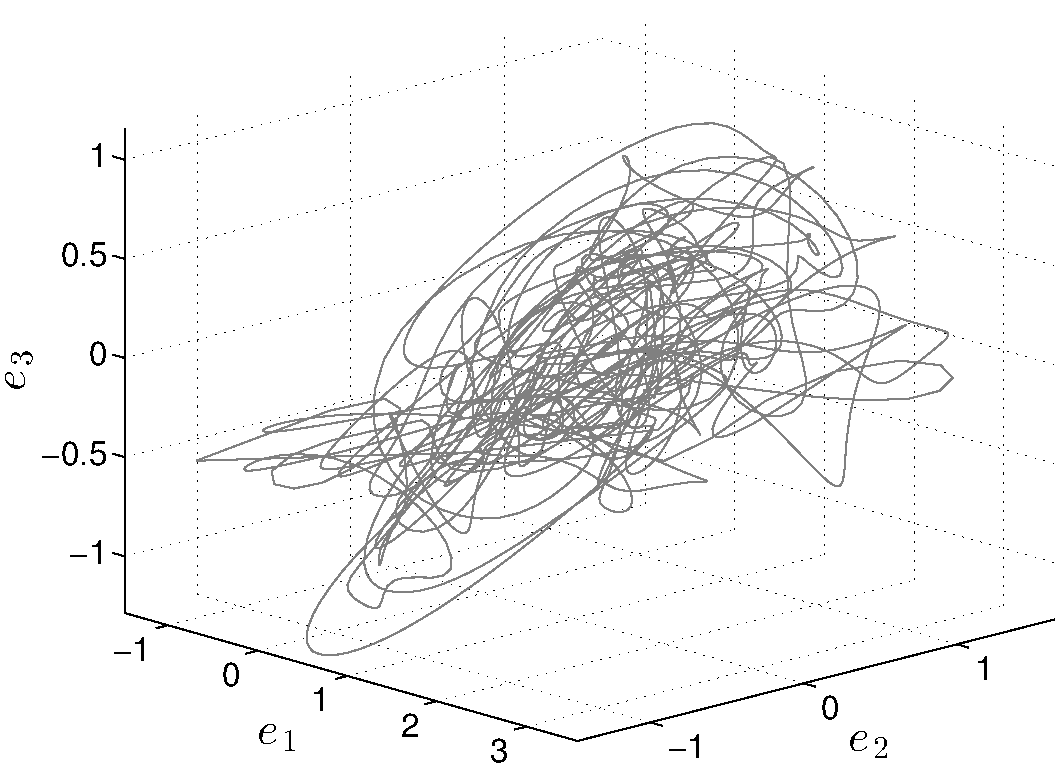
\includegraphics[width=.65\textwidth]{proj_E4E7T2_t300}
\caption{The projection of the ergodic trajectory onto an orthonormal basis
$\{e_1,e_2,e_3\}$ made out of $E_4$, $E_7$ and $T_{2}$. The origin is $E_1$.
Everything is first sliced, then averaged over discrete symmetries.
Ergodic trajectory up to $t=300$ time units.
}
\label{fig:proj_E4E7T2}
\end{figure}
}

\PCpost{2015-06-20}{
I've started drafting a group-theoretic discussion in \refsect{s:KFsymm}. It is
clip and paste, and most of it not ready for prime time, but do try to
implement the orthogonal \statesp\ coordinates \refeq{globalUBframe}
given by the transverse dihedral \Dn{4}\ symmetry (ignoring the parity
transformation for time being). Your projection operator
\refeq{MMFaxis1} presumably corresponds to the fully symmetrized
basis vector.
Writing this takes time (a whole work day
so far), so I'll return to it after we discus it. Let me know if I can
help by explainig anything (can be done by Skype of GHangout).
    }

\MMFpost{2015-06-19}{\refFig{fig:proj_E4E7E13}:
Projection onto a basis within the symmetry-averaged space seems to work.
See the caption for details.
\begin{figure}
\centering
(a)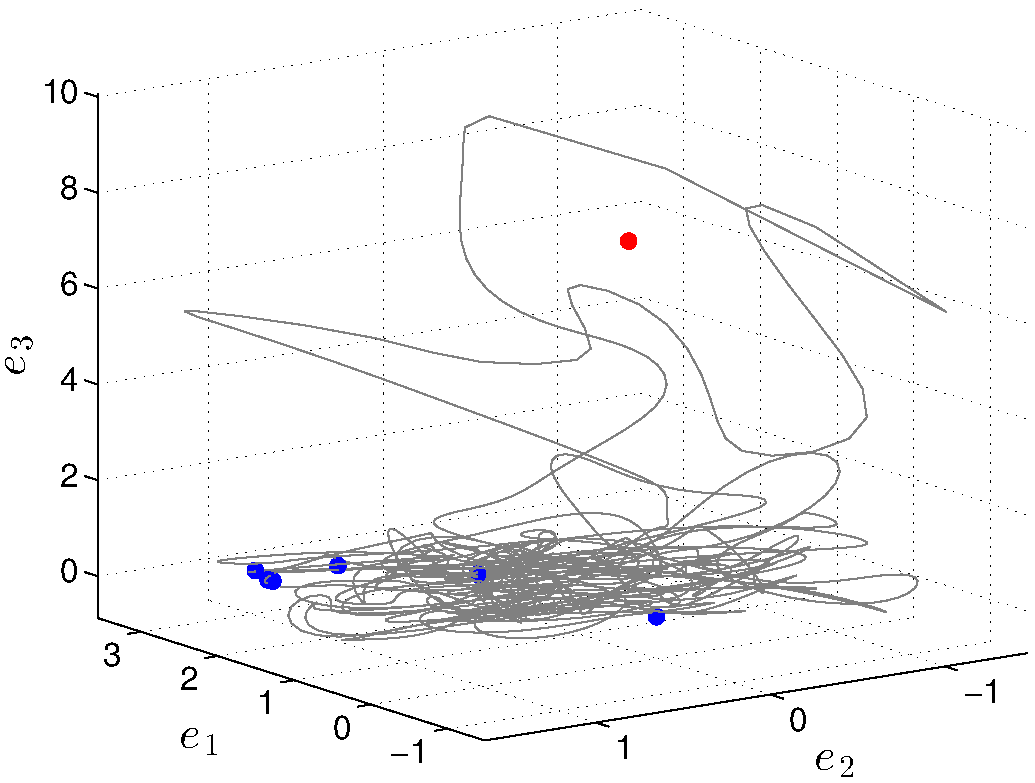
\includegraphics[width=.65\textwidth]{proj_E4E7E13_t300}
(b)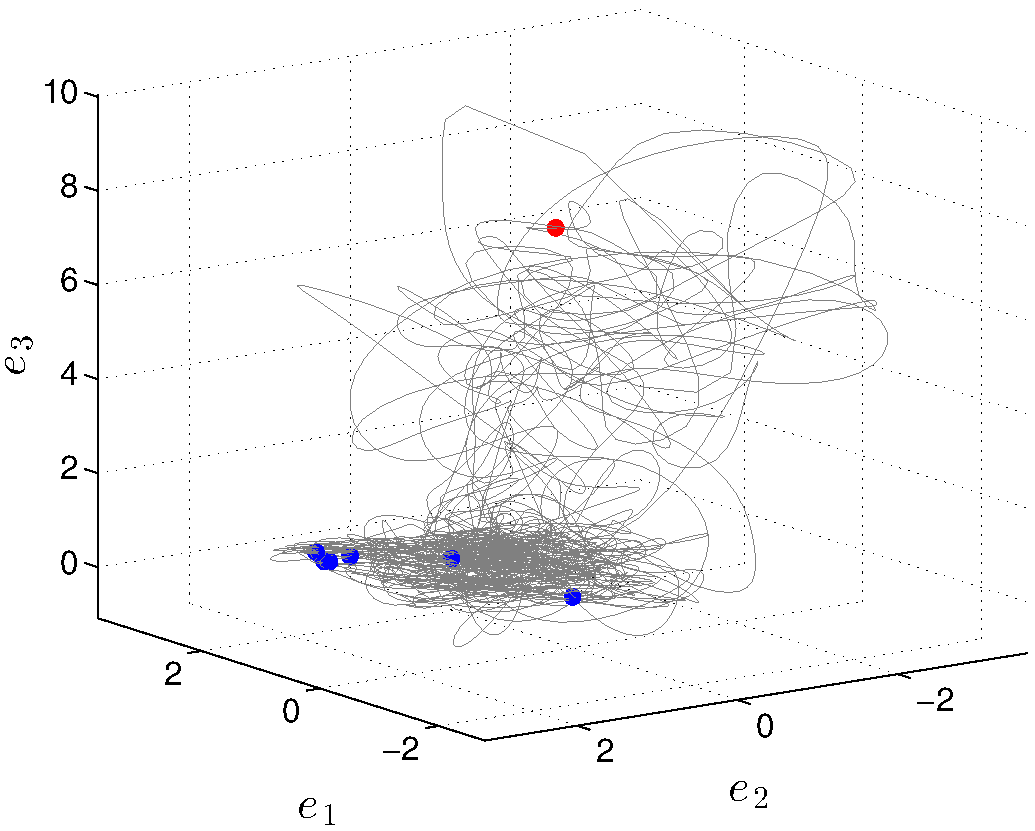
\includegraphics[width=.65\textwidth]{proj_E4E7E13_t1000}
\caption{The projection of the ergodic trajectory onto an orthonormal basis
$\{e_1,e_2,e_3\}$ made out of $E_4$, $E_7$ and $E_{13}$. The origin is $E_1$.
Everything is first sliced, then averaged over discrete symmetries.
The blue dots show EQ and TWs with low energy dissipation.
The red dot is $E_{13}$ with relatively large energy dissipation.
For clarity, only a segment of the ergodic trajectory is shown.
(a) Ergodic trajectory up to $t=300$ time units.
(b) Ergodic trajectory up to $t=1000$ time units.
}
\label{fig:proj_E4E7E13}
\end{figure}
}

\MMFpost{2015-06-08}{\refFig{fig:TW_kolm_R40}:
The first two traveling waves found by the adjoint.
\begin{figure}
\centering
(a)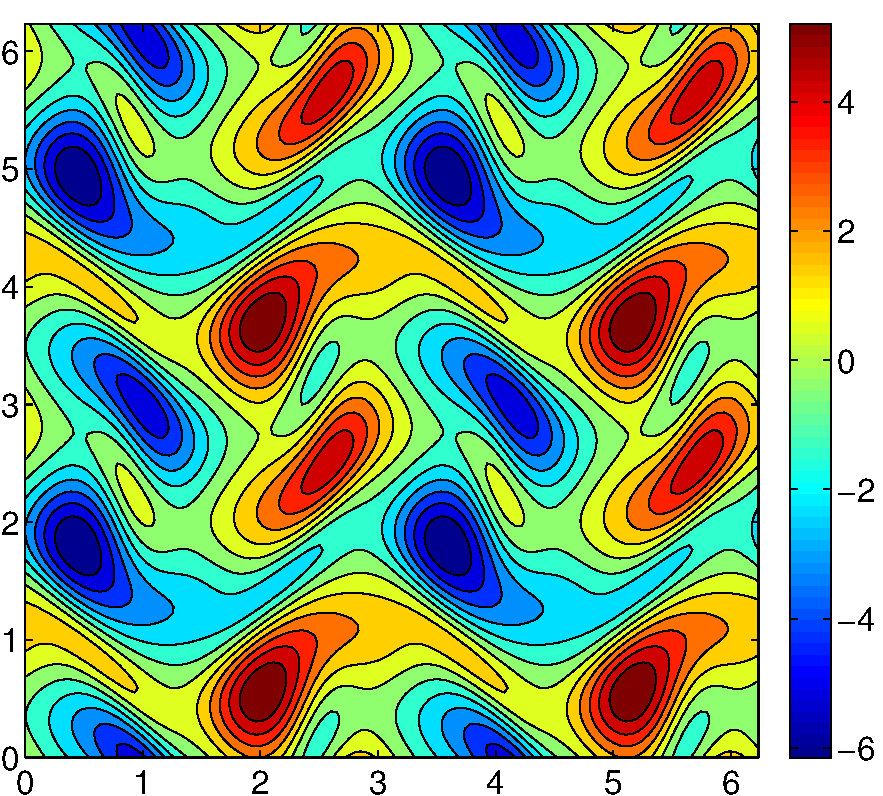
\includegraphics[width=.45\textwidth]{R40_TW1}		
(b)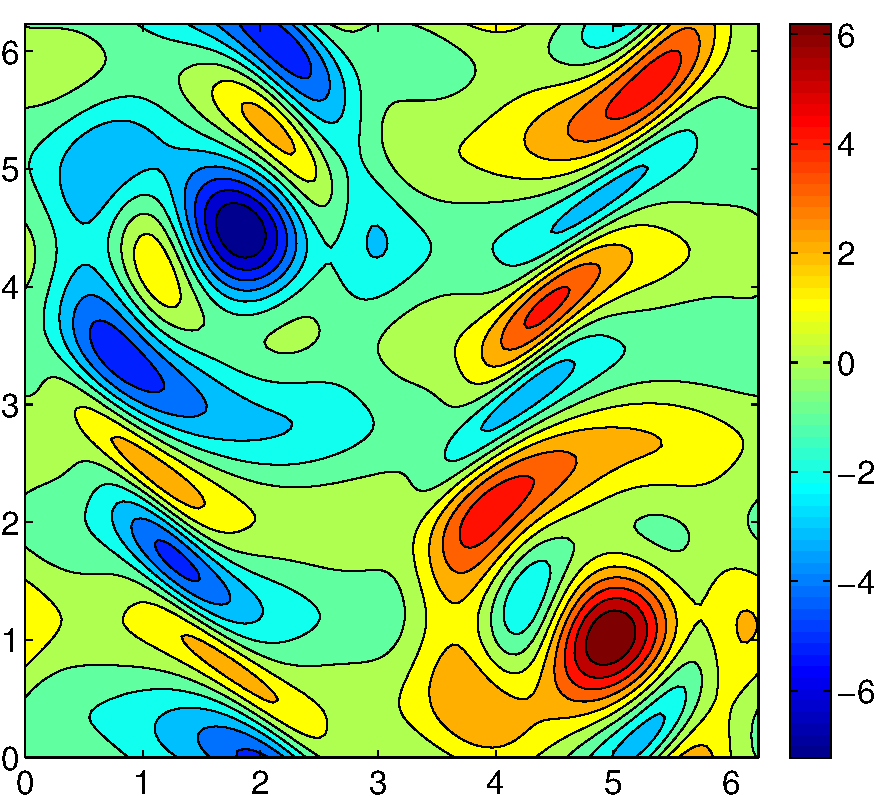
\includegraphics[width=.45\textwidth]{R40_TW2}
(c)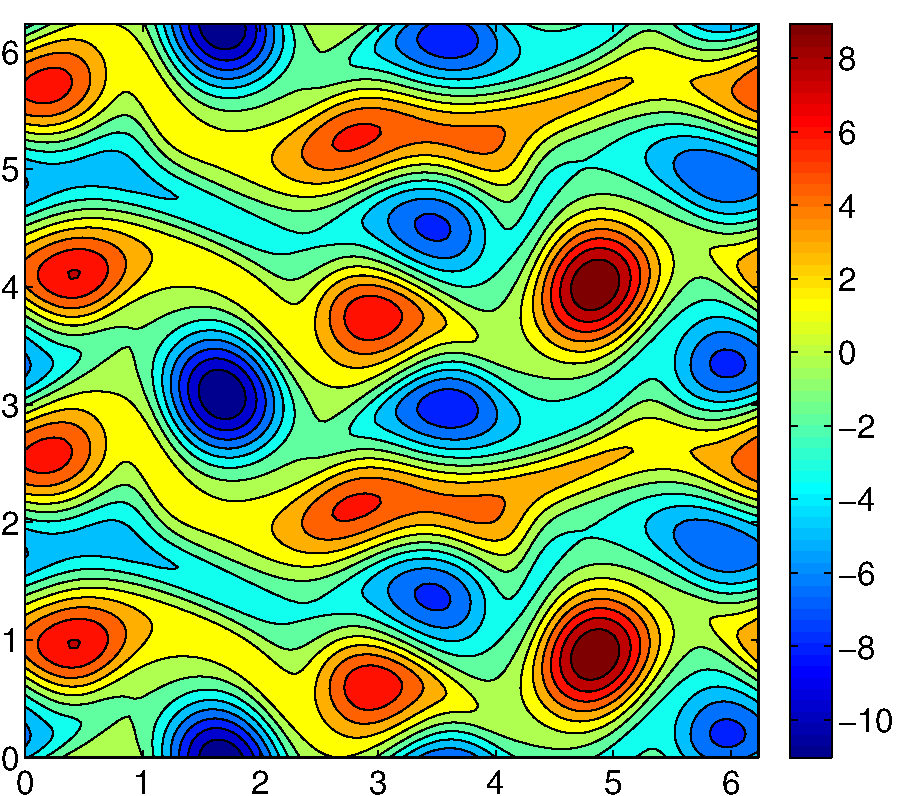
\includegraphics[width=.45\textwidth]{R40_TW3}
(d)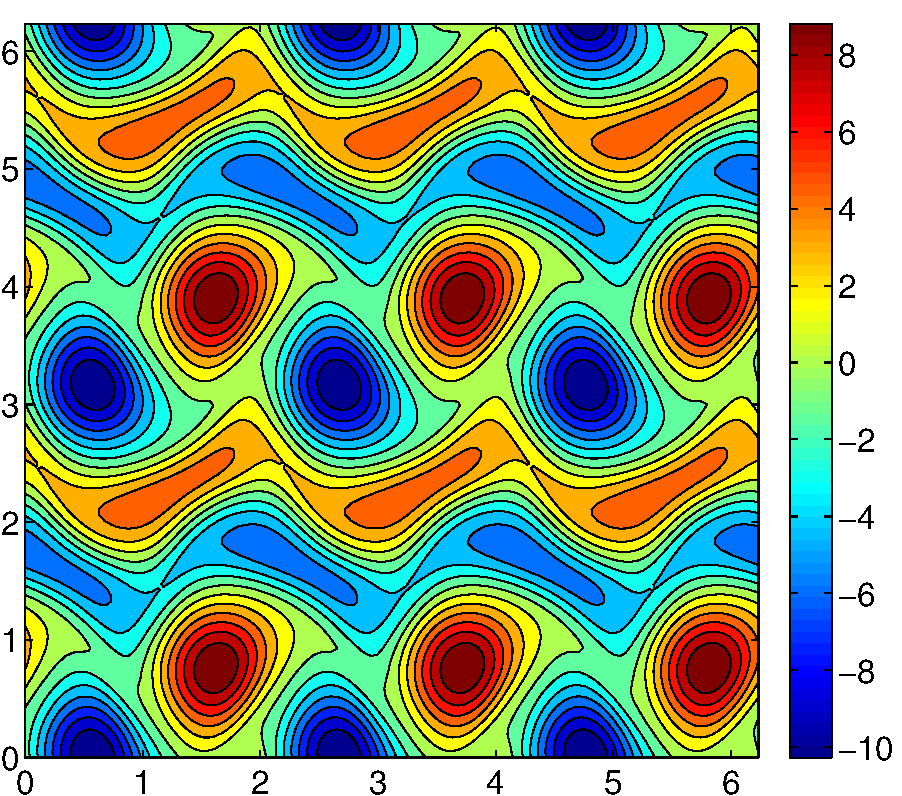
\includegraphics[width=.45\textwidth]{R40_TW4}
(e)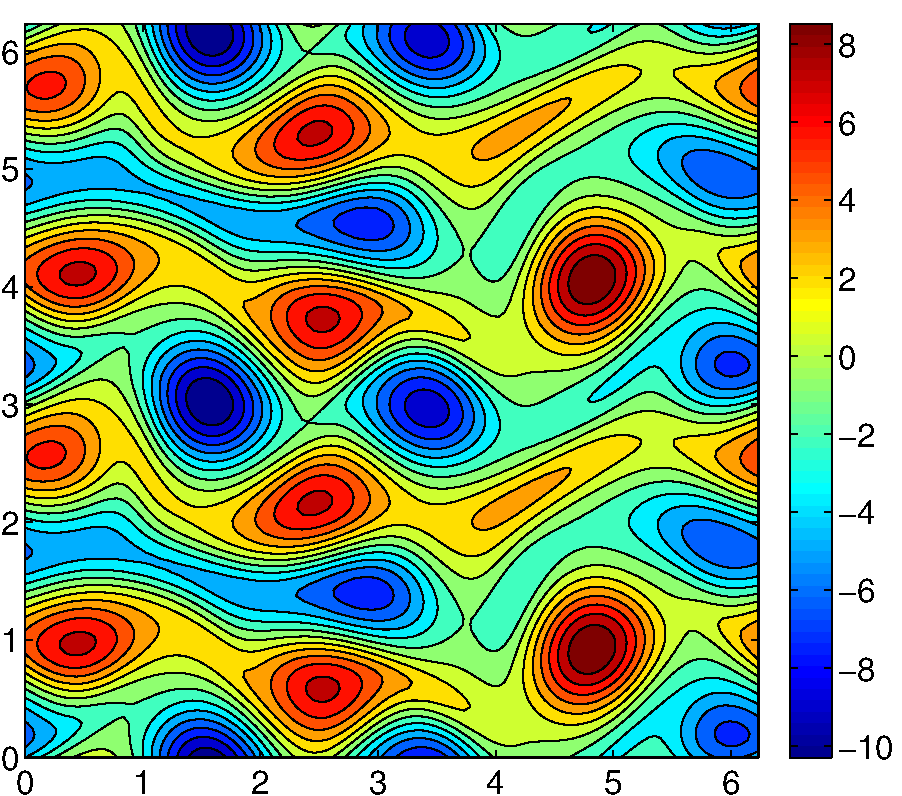
\includegraphics[width=.45\textwidth]{R40_TW5}
(f)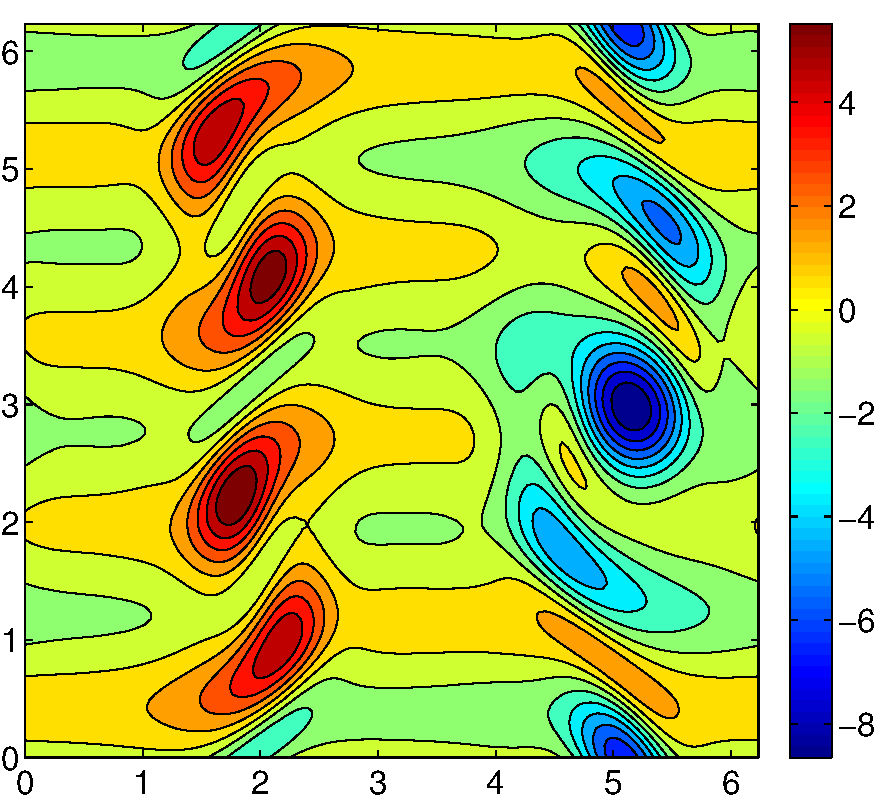
\includegraphics[width=.45\textwidth]{R40_TW6}
\caption{$\mbox{Re}=40$ and resolution $128\times 128$.
(a) Wave speed $c=0.018264$.
(b) Wave speed $c=0.019782$.
(c) Wave speed $c=0.030619$.
(d) Wave speed $c=0.052661$.
(e) Wave speed $c=0.042231$.
(f) Wave speed $c=0.002078$.
Panel (b) coincides with T1 found by CK13.}
\label{fig:TW_kolm_R40}
\end{figure}
}

\MMFpost{2015-05-07}{
\refFig{fig:ID_R40}: ID plot for the Kolmogorov flow at $\mbox{Re}=40$.
\begin{figure}
\centering
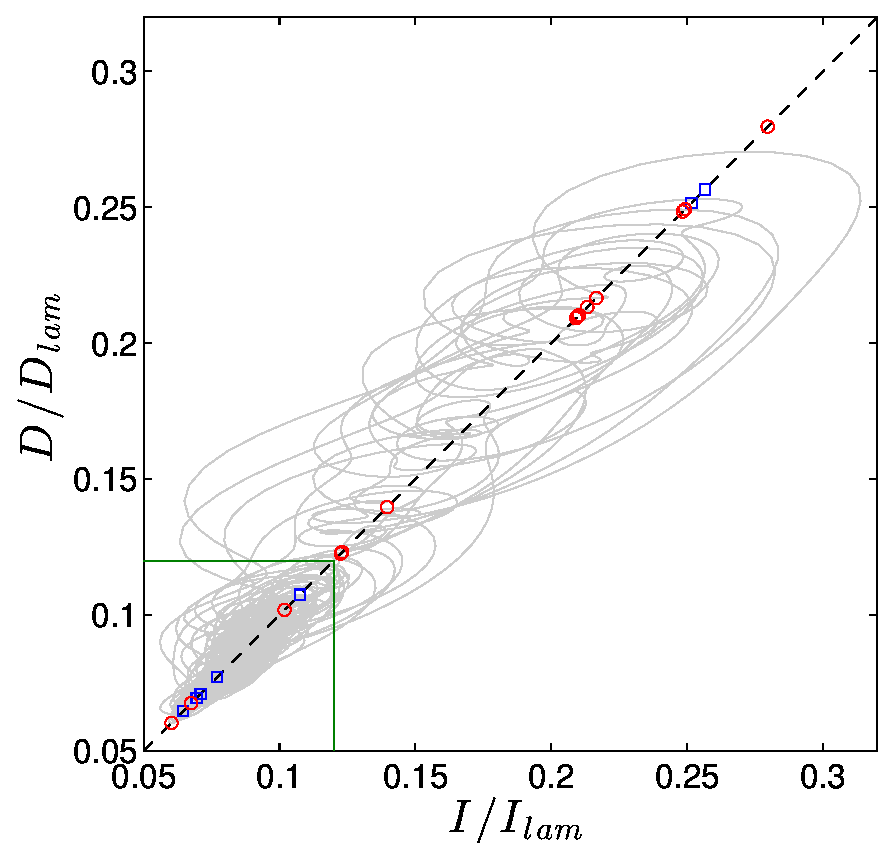
\includegraphics[width=.75\textwidth]{ID_R40}		
\caption{$\mbox{Re}=40$. Gray: Ergodic trajectory. Black star: initial condition for the
ergodic trajectory. Dashed line: $I=D$ line. Dots: Equilibria shown in
\reffig{fig:Kol_R40_E3}.}
\label{fig:ID_R40}
\end{figure}
}
	
\MMFpost{2015-05-05}{Figures \ref{fig:kol_R100_EQ}: Equilibrium for $Re=100$.
	\begin{figure}
		\centering
		(a)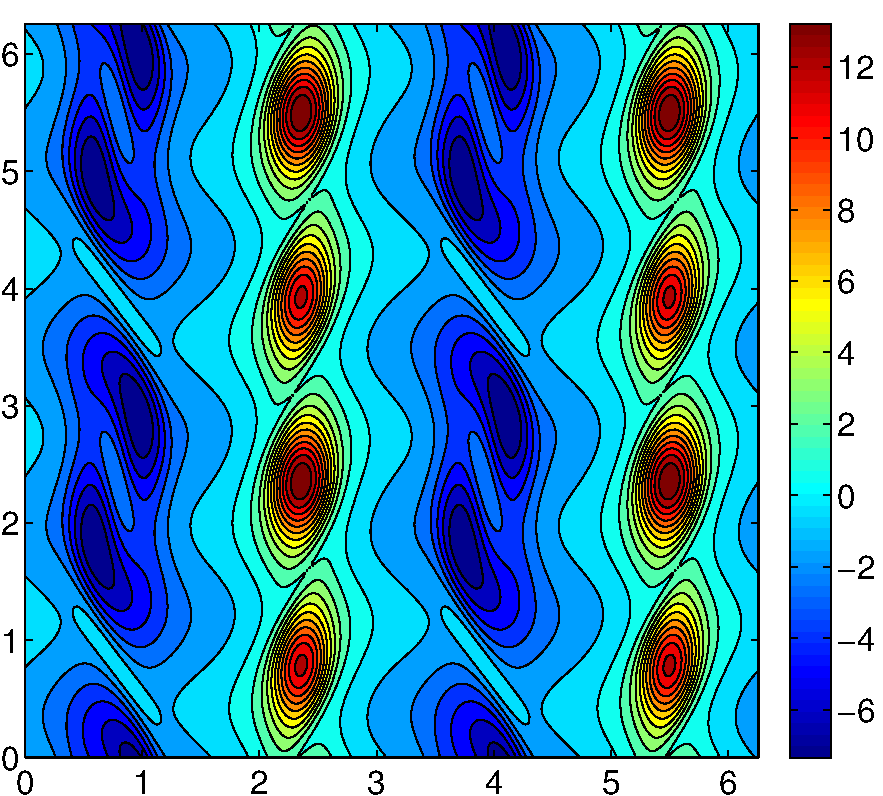
\includegraphics[width=.45\textwidth]{Kol_R100_n256_vort_E2}		
		(b)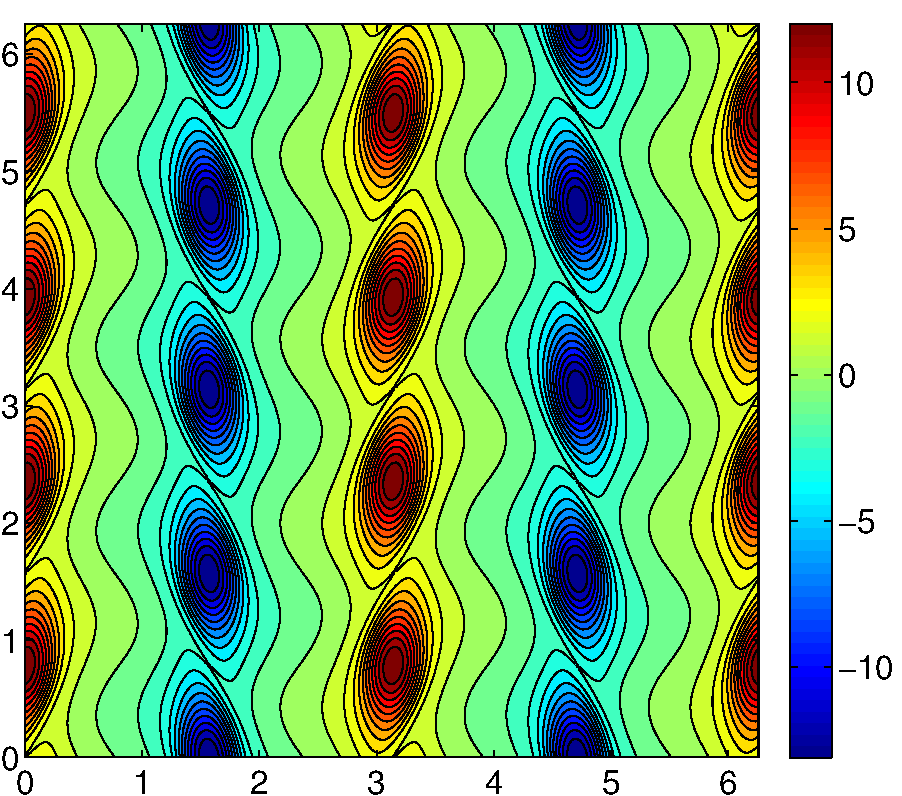
\includegraphics[width=.45\textwidth]{Kol_R100_n256_vort_E4-2sin}
		\caption{$\mbox{Re}=100$ and resolution $256\times 256$. (a) Initial condition
		$\mathbf u(x,y)=(2\cos(2y),2\cos(2x))$ converged to
			equilibrium with residue $6\times 10^{-8}$. (b) Initial condition
			$\mathbf u(x,y)=(\sin(4y),4.5\sin(2x))$ converged to
			equilibrium with residue $1\times 10^{-9}$.}
		\label{fig:kol_R100_EQ}
	\end{figure}
}

\MMFpost{2015-05-05}{\refFig{fig:kol_R80_E2}(b): New equilibrium at $Re=80$ and
\refFig{fig:kol_R60_E1}(c,d): New equilibrium at $Re=60$.
}

\MMFpost{2015-05-04}{Figures \ref{fig:kol_R60_E1}(b) and \ref{fig:kol_R80_E2}:
	New equilibria for $\mbox{Re}=60$ and $80$.
	\begin{figure}
		\centering
        (a)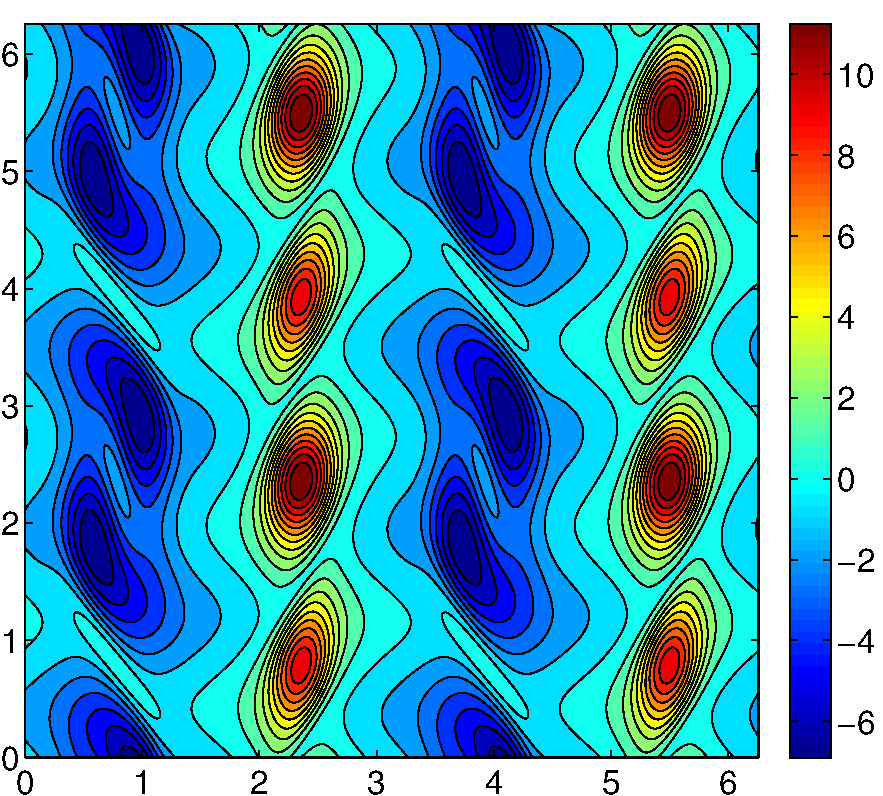
\includegraphics[width=.45\textwidth]{Kol_R80_n256_vort_E2}
        (b)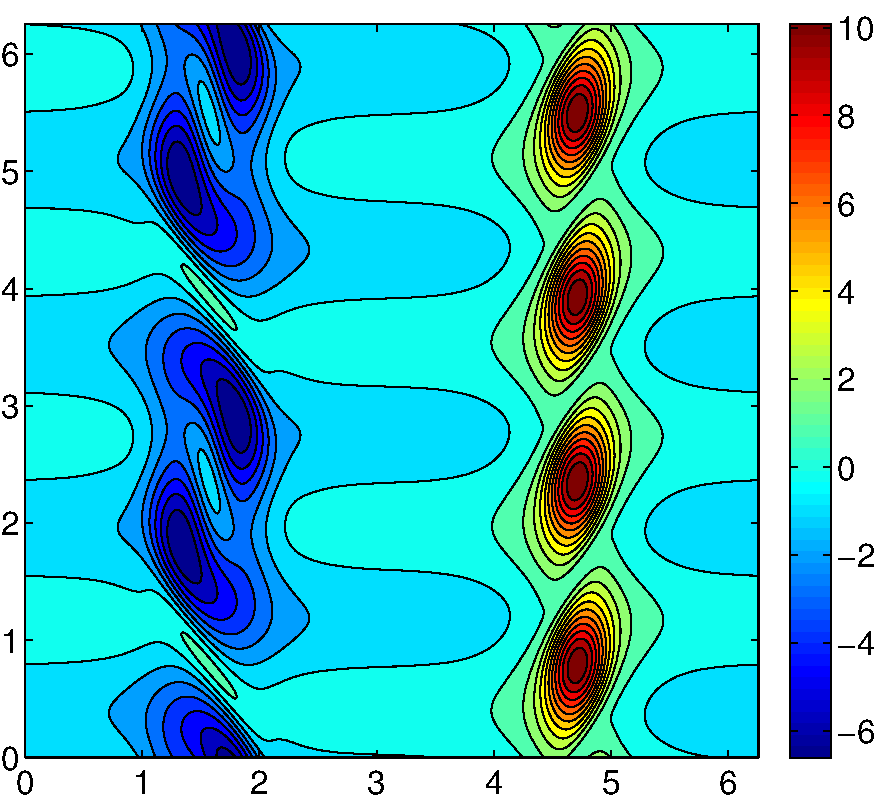
\includegraphics[width=.45\textwidth]{Kol_R80_n256_vort_E2-1}
		\caption{$\mbox{Re}=80$ and resolution $256\times 256$. (a) The adjoint-Newton
		hybrid with initial condition $\mathbf u(x,y)=(2\cos(2y),2\cos(2x))$ converged to
		equilibrium with residue $4\times 10^{-8}$. (b) Initial condition $\mathbf
		u(x,y)=(2\cos(2y),2\cos(x))$ with residue $9\times 10^{-9}$.}
		\label{fig:kol_R80_E2}
	\end{figure}
}	
	
\MMFpost{2015-05-03}{Predrag, could you please create a paper template for the adjoint
method. I'll start filling it up as we go. Most of the theory is
in place, so I can start writing that part immediately.
}
\MMFpost{2015-05-01}{\refFig{fig:kol_R60_E1}: Equilibrium solution for the Kolmogorov
flow at $Re=60$ computed by the adjoint equation.
\begin{figure}
	\centering
	(a)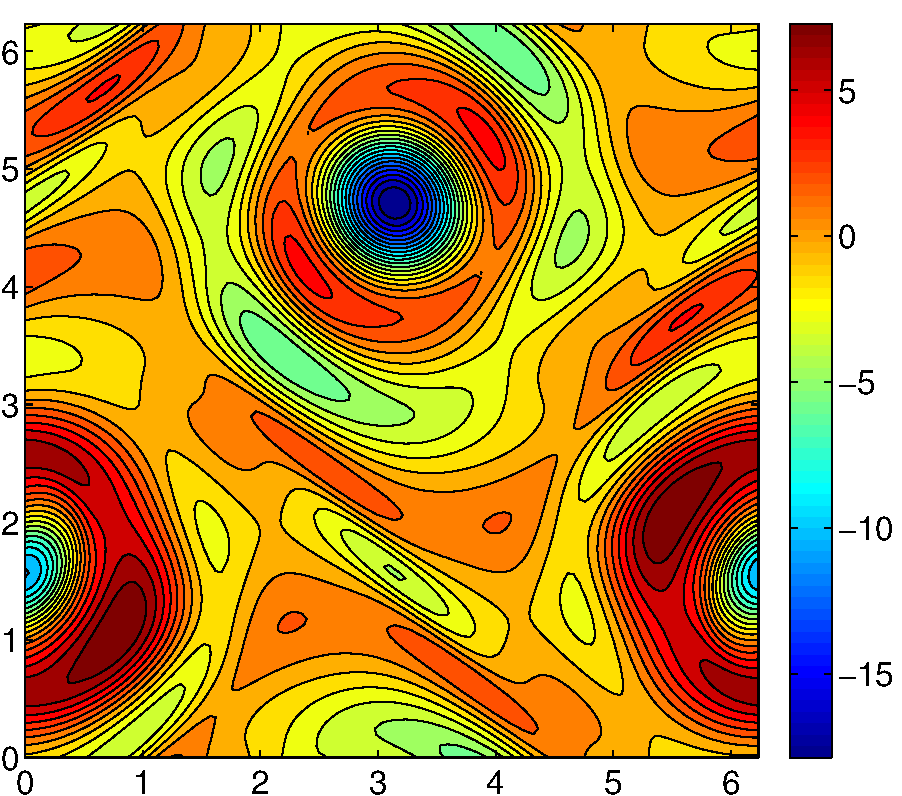
\includegraphics[width=.45\textwidth]{Kol_R60_n128_vort_E1}
    (b)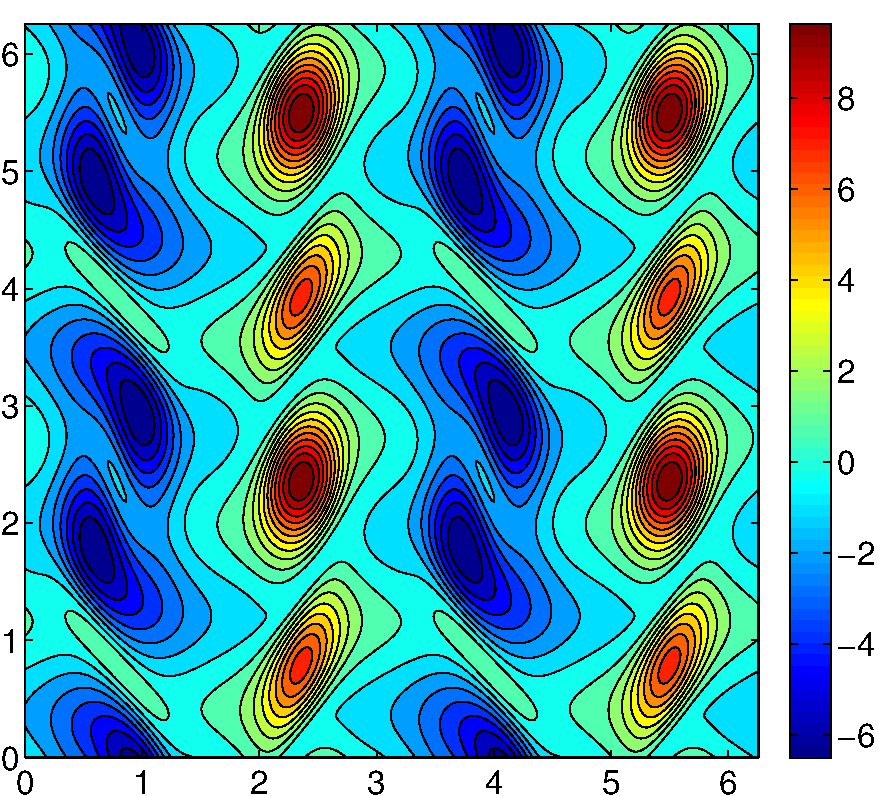
\includegraphics[width=.45\textwidth]{Kol_R60_n256_vort_E2}\\
    (c)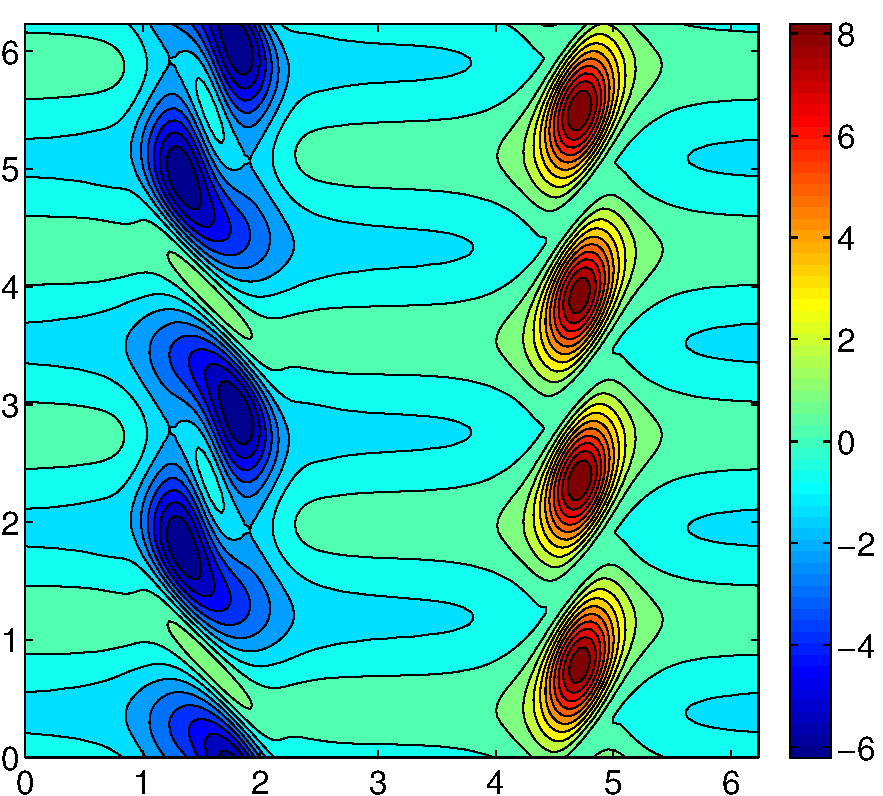
\includegraphics[width=.45\textwidth]{Kol_R60_n128_vort_E2-1}
    (d)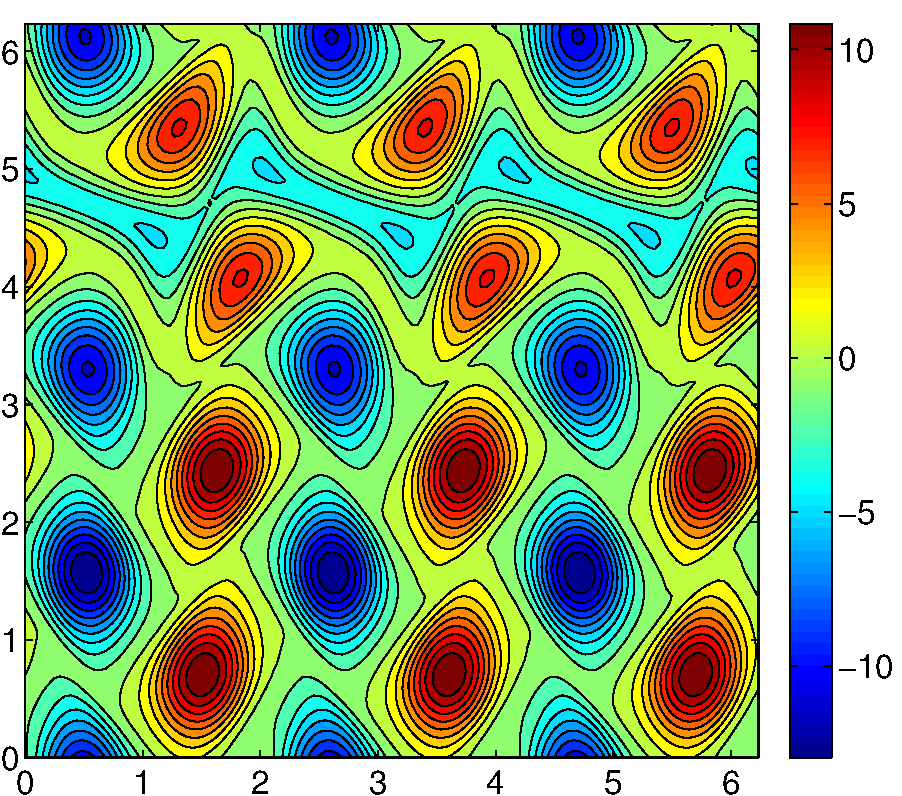
\includegraphics[width=.45\textwidth]{Kol_R60_n128_vort_E3}
	\caption{$\mbox{Re}=60$ (a) The adjoint equation integrated with initial condition
	$\mathbf u(x,y)=(2\cos(y),2\cos(x))$ for $10^4$ time units (took 2 minutes) then
	switched to Newton-GMRES to reduce the residue to $4\times 10^{-13}$ after $8$
		iterations. Resolution $128\times 128$. (b) The initial
		condition was $\mathbf u(x,y)=(2\cos(2y),2\cos(2x))$ and resolution $256\times
		256$. (c) The initial condition was $\mathbf u(x,y)=(2\cos(2y),2\cos(x))$ and
		resolution $128\times 128$ converged with residue $3\times 10^{-8}$. (d) Initial
		condition $\mathbf u(x,y)=(2\cos(3y),2\cos(3x))$ and resolution $128\times 128$
		converged with residue $1\times 10^{-8}$.}
	\label{fig:kol_R60_E1}
\end{figure}
}
	
\MMFpost{2015-04-22}{I contacted Rich Kerswell regarding the equilibrium solutions I find
for Kolmogorov flow but they did not find. As I suspected, they look for equilibria using
recurrences. As a result, they miss all the equilibria in the shift-invariant subspaces.
I copy the relevant part of his response to my email:

Rich Kerswell: ``I think the quick answer to your question is we didn't find many
equilibria in Chandler \& Kerswell by the approach taken there i.e. recurrent flow
analysis."
}

\MMFpost{2015-04-21}{There seems to be a zoo of shift-invariant equilibria. See
\reffig{fig:Kol_R40_E3}
\begin{figure}
	\centering
	(a)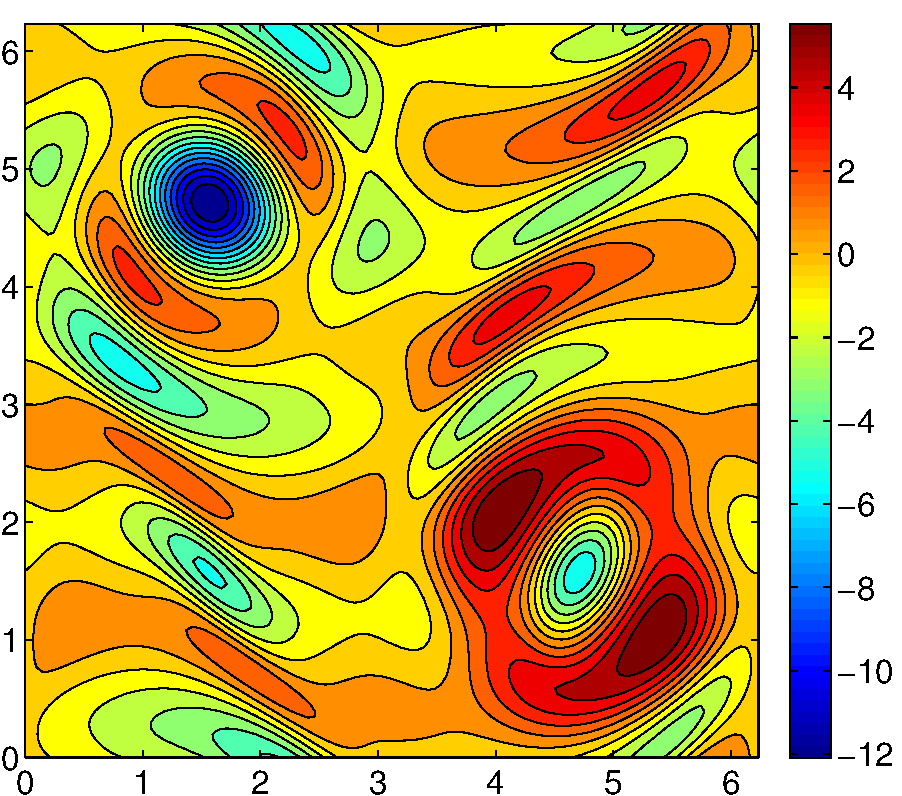
\includegraphics[width=.45\textwidth]{Kol_R40_n128_vort_E1}
	(b)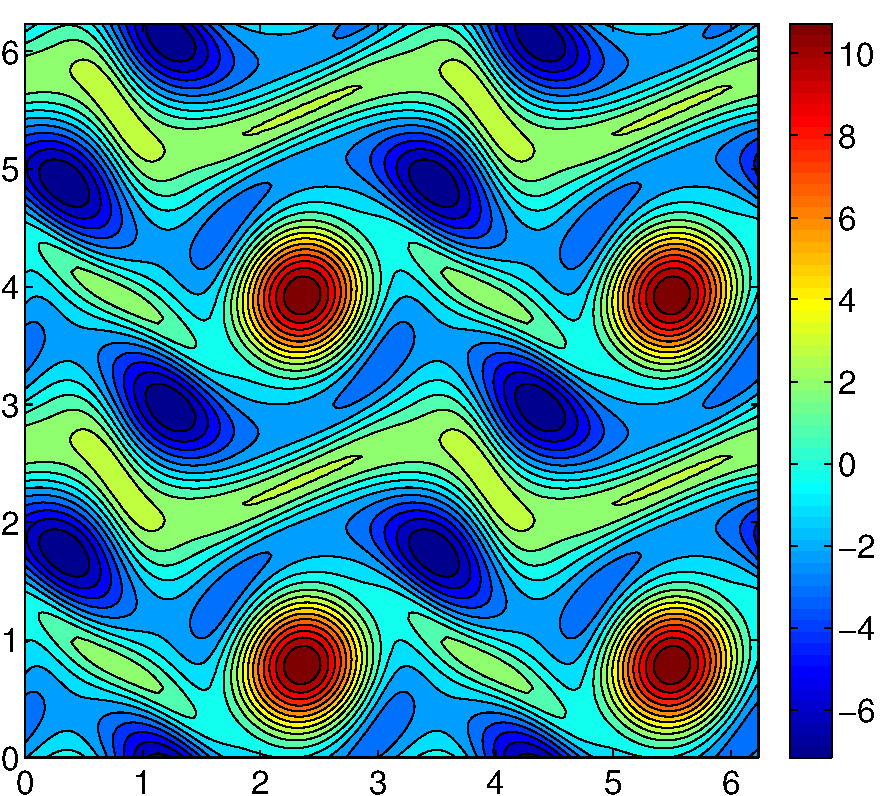
\includegraphics[width=.45\textwidth]{Kol_R40_n128_vort_E2}\\
	(c)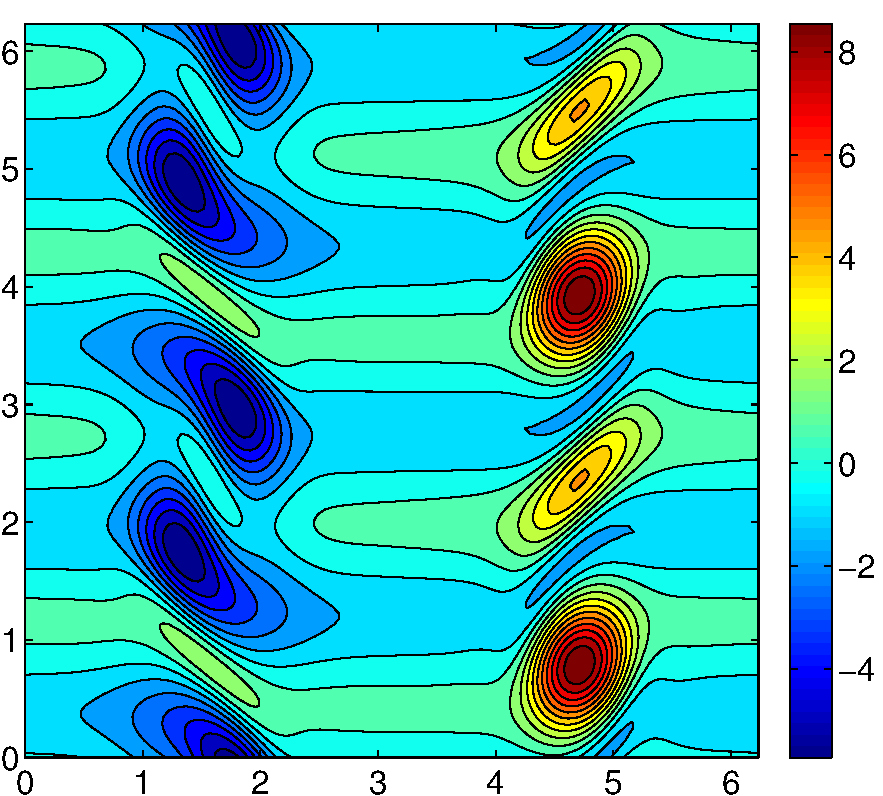
\includegraphics[width=.45\textwidth]{Kol_R40_n128_vort_E2-1}
	(d)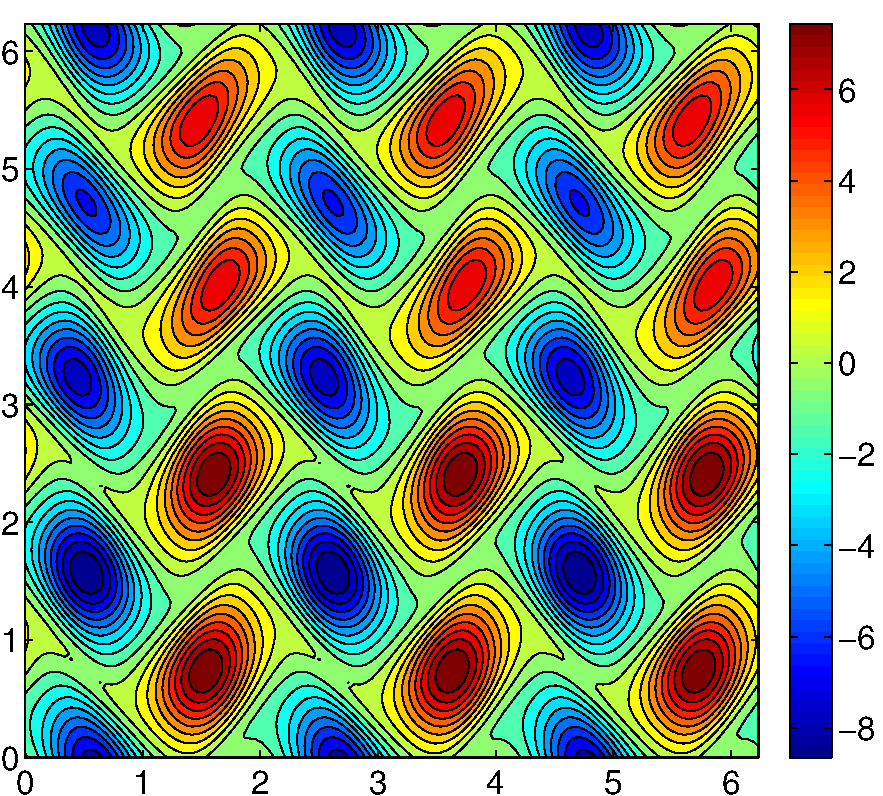
\includegraphics[width=.45\textwidth]{Kol_R40_n128_vort_E3}
	(e)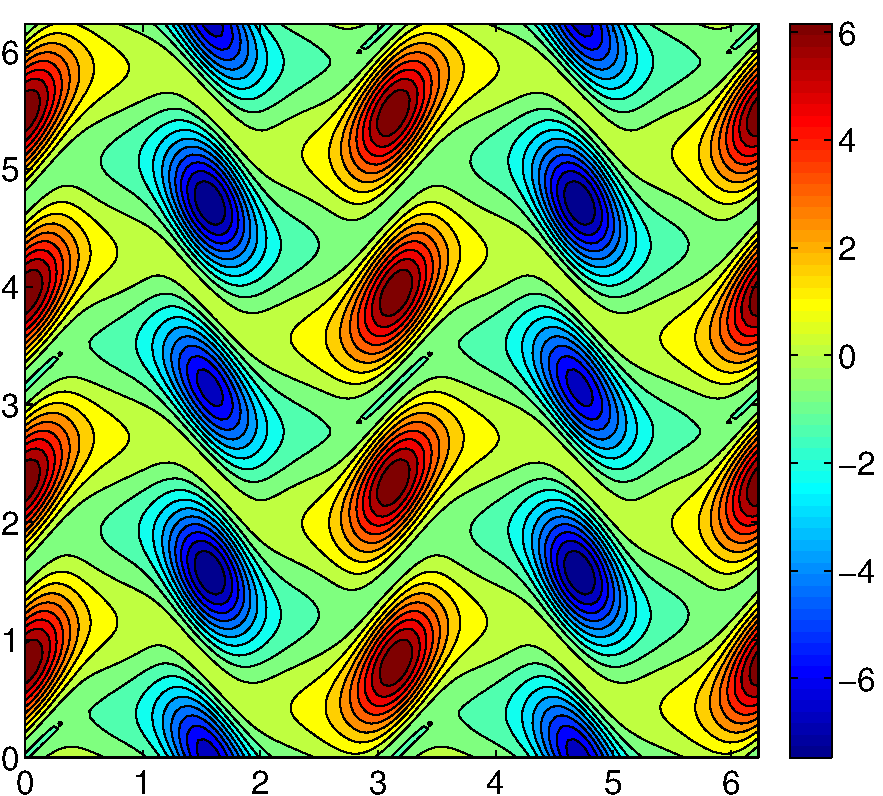
\includegraphics[width=.45\textwidth]{Kol_R40_n128_vort_E2sin}
    (f)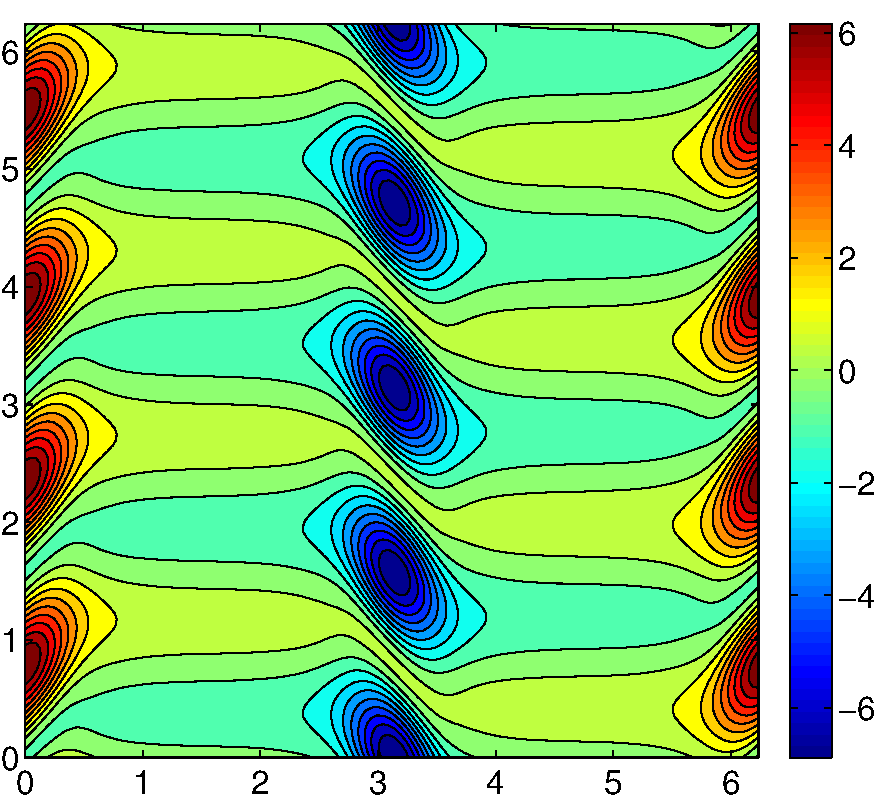
\includegraphics[width=.45\textwidth]{Kol_R40_n128_vort_E4-1sin}
	\caption{$Re=40$ and resolution $128^2$.
		(a) Initial condition $\mathbf
		u(x,y)=(2\cos(y),2\cos(x))$ converged with residue $5\times 10^{-13}$.
		(b) Initial condition $\mathbf u(x,y)=(2\cos(2y),2\cos(2x))$ converged with
		residue $1\times 10^{-13}$.
		(c) Initial condition $\mathbf
		u(x,y)=(2\cos(2y),2\cos(x))$ converged with residue $1\times 10^{-9}$
		(d) Initial condition
		$\mathbf u(x,y)=(2\cos(3y),2\cos(3x))$ converged with residue $4\times 10^{-13}$.
		(e) Initial condition
		$\mathbf u(x,y)=(\sin(2y),\sin(2x))$ converged with residue $4\times 10^{-9}$.
		(f) Initial condition
		$\mathbf u(x,y)=(0.5\sin(4y),3\sin(x))$ converged with residue $2\times 10^{-9}$.
		}
	\label{fig:Kol_R40_E3}
\end{figure}
\begin{figure}
	\centering
	(g)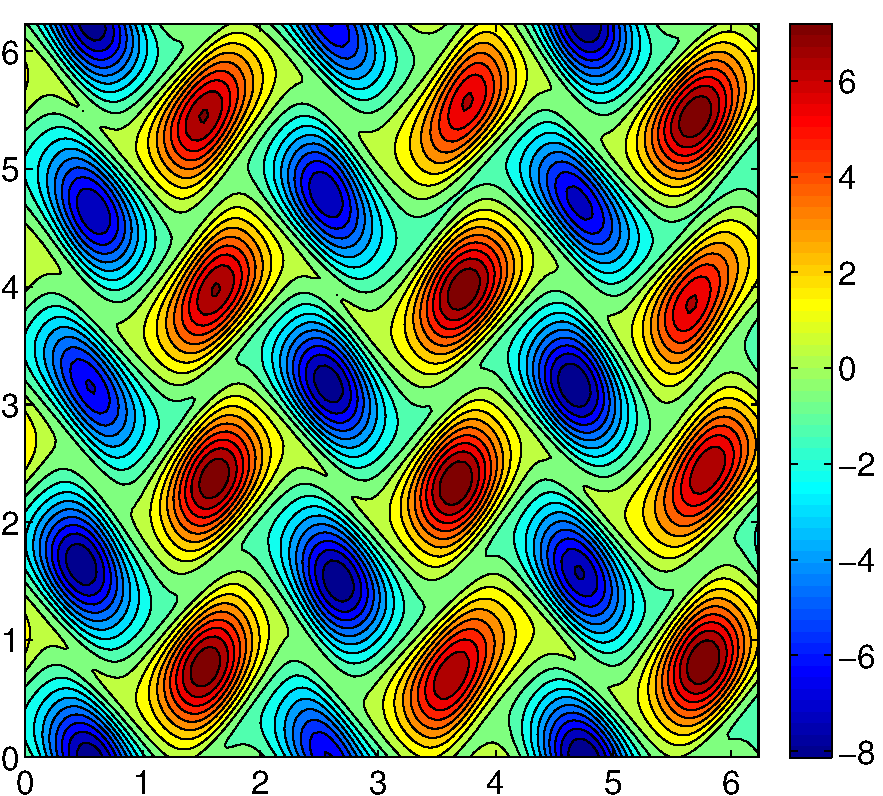
\includegraphics[width=.45\textwidth]{Kol_R40_n128_vort_E23-23}
    (h)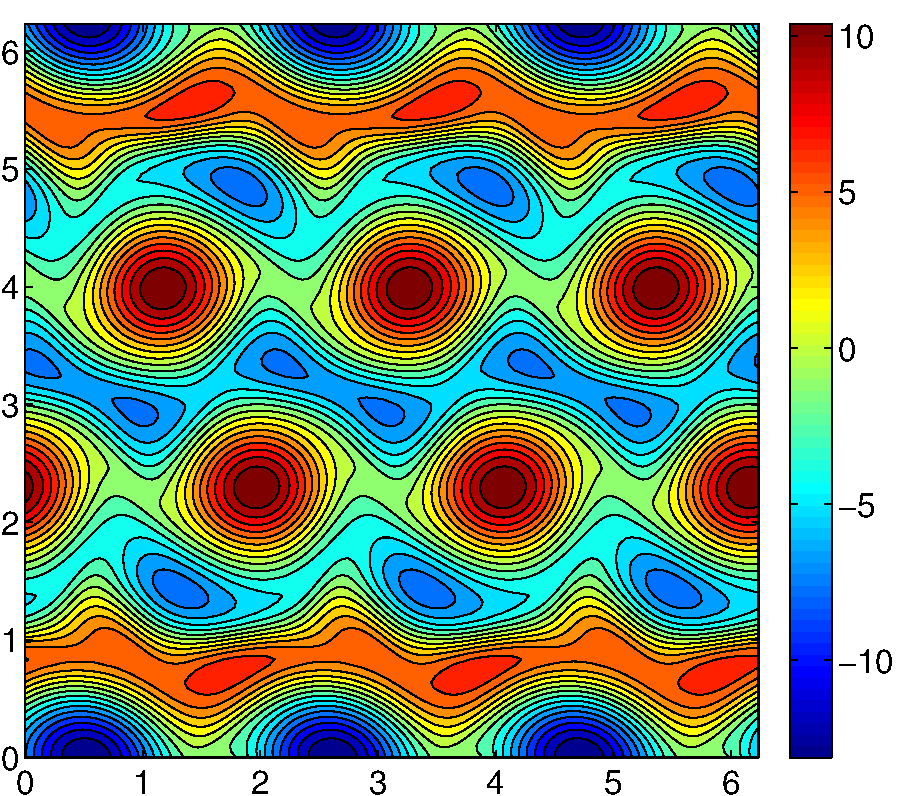
\includegraphics[width=.45\textwidth]{Kol_R40_n128_vort_E9}
    (i)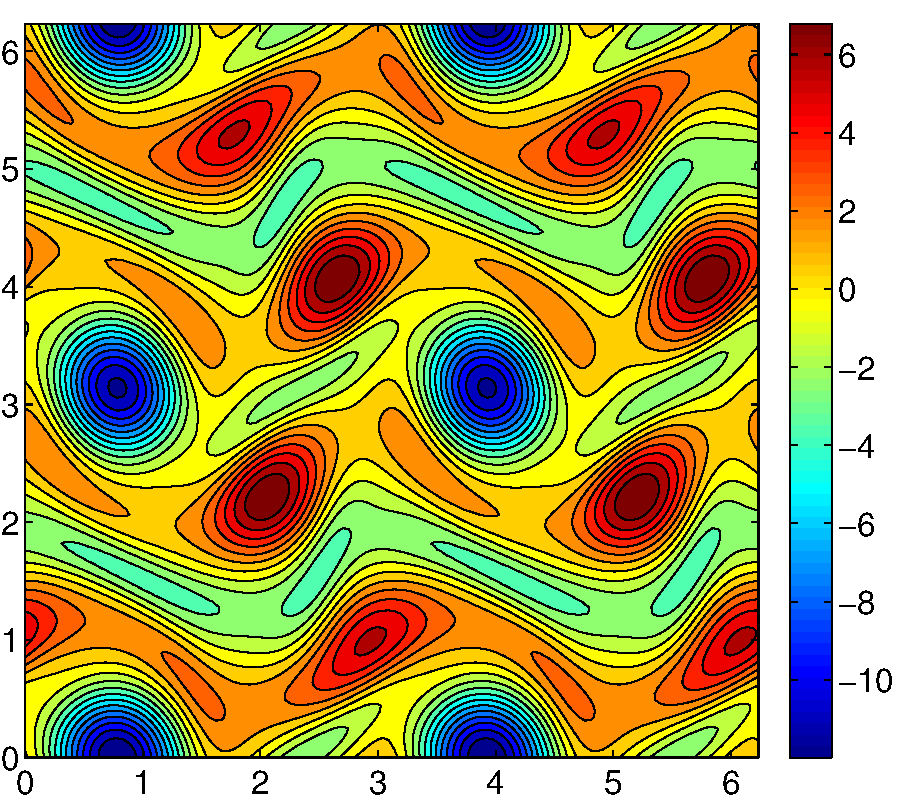
\includegraphics[width=.45\textwidth]{Kol_R40_n128_vort_E10}
    (j)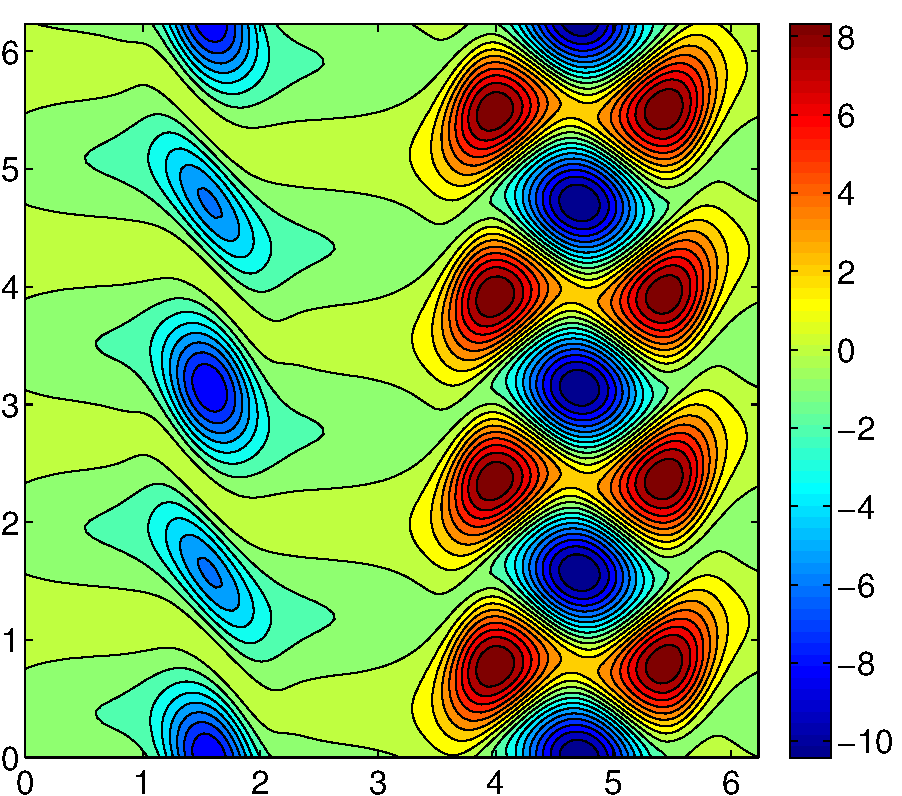
\includegraphics[width=.45\textwidth]{Kol_R40_n128_vort_E12}
    (k)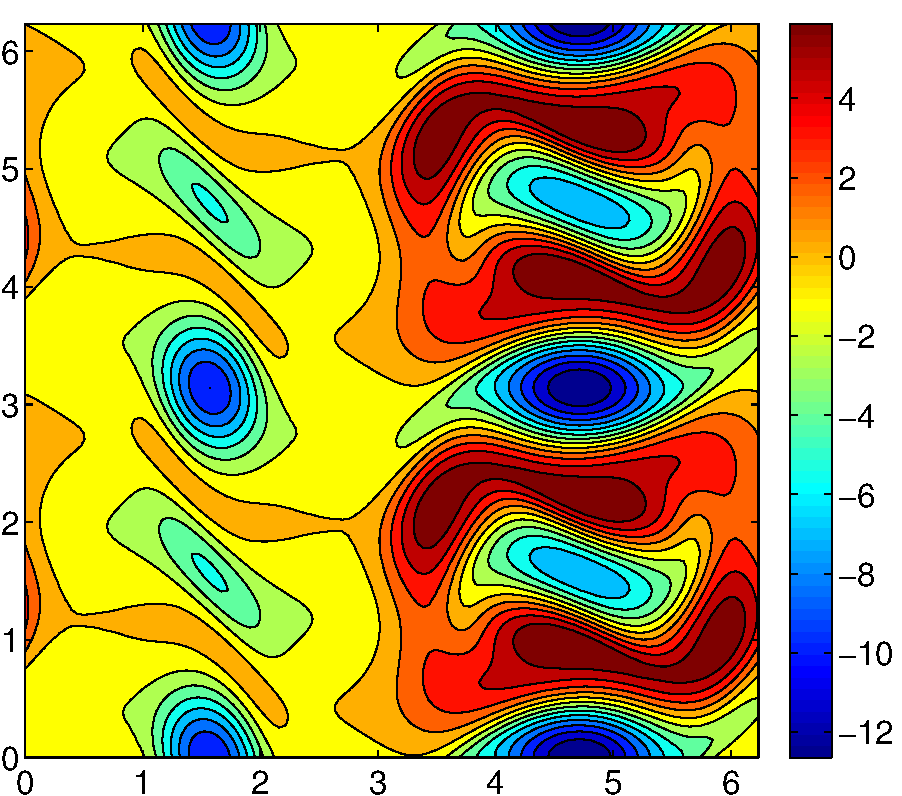
\includegraphics[width=.45\textwidth]{Kol_R40_n128_vort_E15}
	\caption{Continued from \reffig{fig:Kol_R40_E3}. $Re=40$ and resolution $128^2$.
		(g) Initial condition $\mathbf
		u(x,y)=(\sin(2y)+\sin(3y),2\sin(2x)+2\sin(3x))$ converged with residue
		$5\times 10^{-9}$. (h) Initial condition $u(x,y)=(\sin(y),\cos(3x))$ converged
		with residue $2.4\times 10^{-10}$ (i) Initial condition
		$u(x,y)=(\sin(y),\cos(2x))$ converged
		with residue $8\times 10^{-11}$. (j) Initial condition
		$u(x,y)=(\sin(2y),\cos(x))$ converged
		with residue $2\times 10^{-10}$.
		(k) Initial condition
		$u(x,y)=(\sin(2y),\cos(x))$ converged
		with residue $1.5\times 10^{-9}$, only Newton-GMRES was used.
			}
\end{figure}
}

\MMFpost{2015-04-21}{\refFig{fig:Kol_R40_E2}: A new equilibrium solution of Kolmogorov
flow that Chandler \& Kerswell (2013) did not find (or did not report).
\begin{figure}
	\centering
	(a)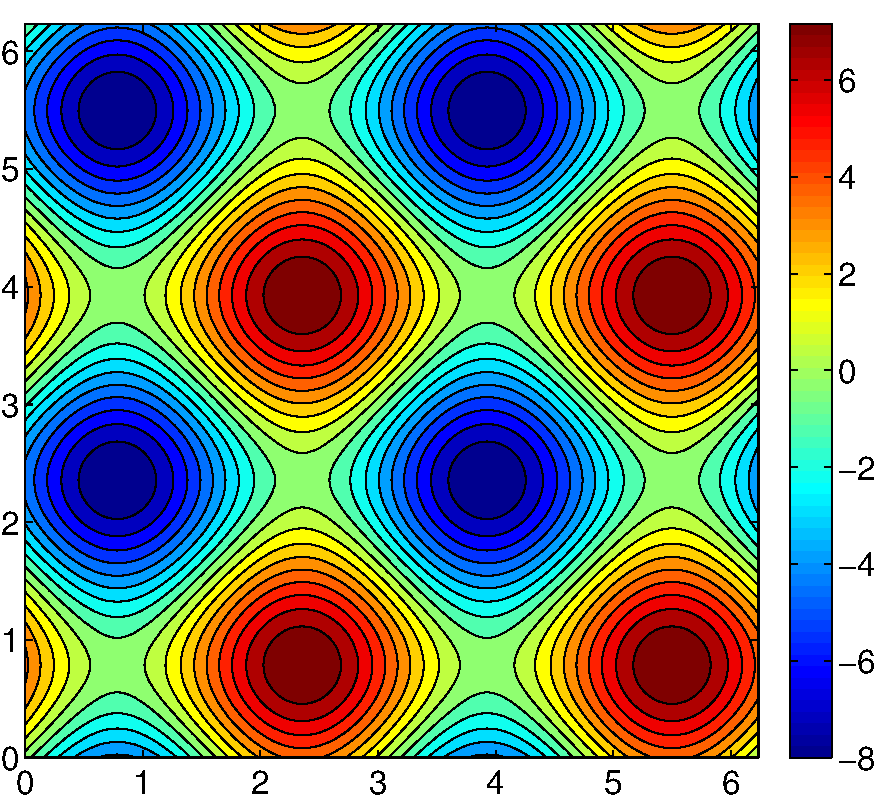
\includegraphics[width=.45\textwidth]{Kol_R40_n128_vort_E2_t0}\\
	(b)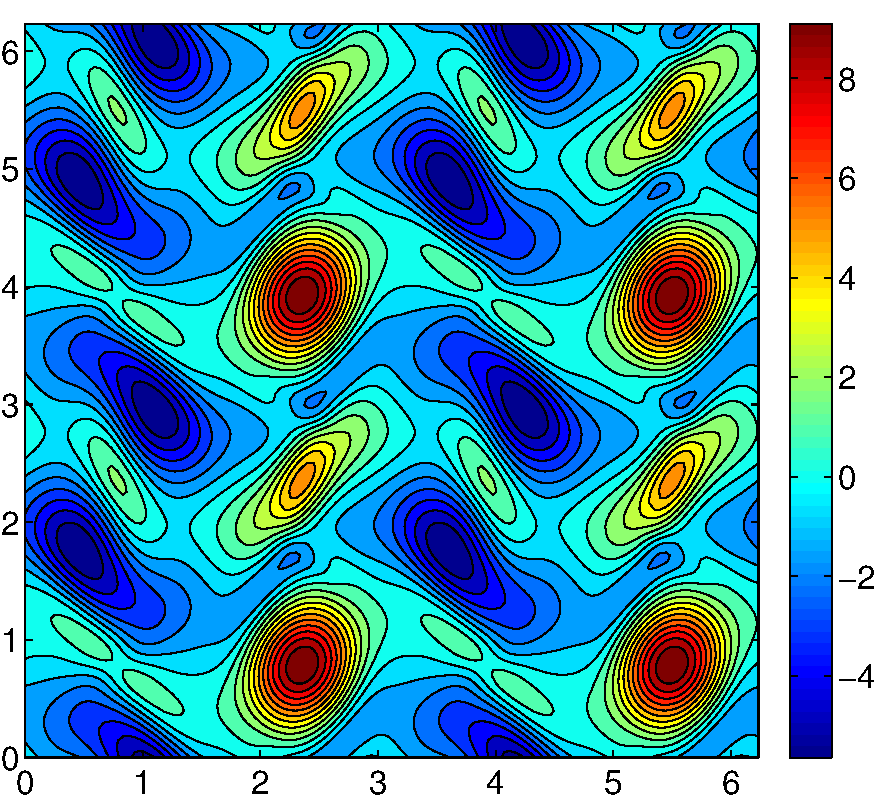
\includegraphics[width=.45\textwidth]{Kol_R40_n128_vort_E2_adj}
    (c)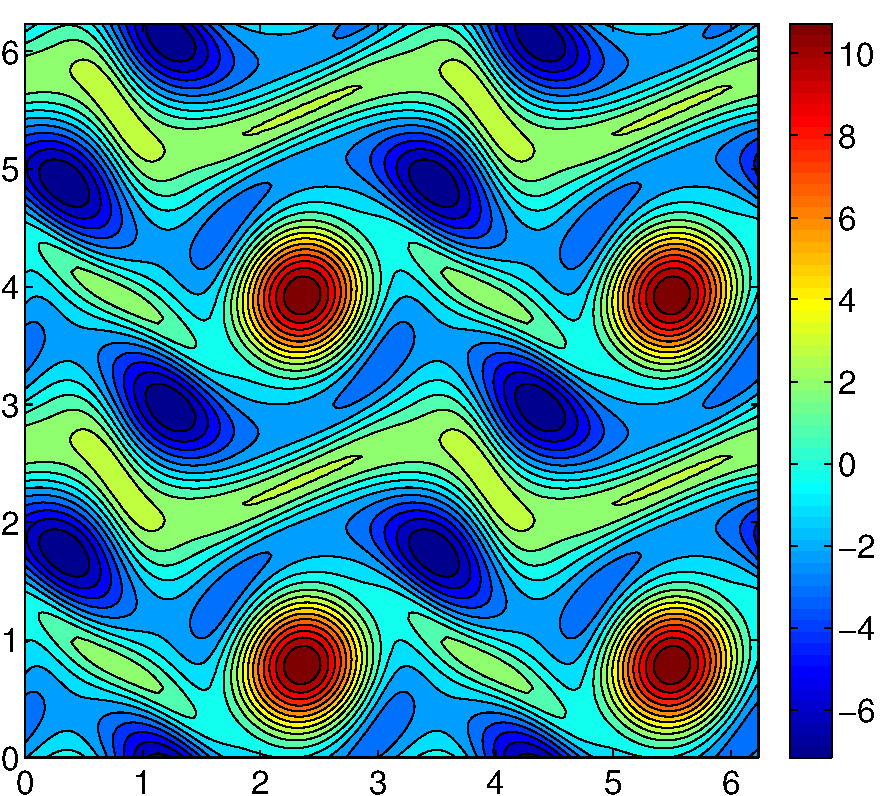
\includegraphics[width=.45\textwidth]{Kol_R40_n128_vort_E2}
	\caption{A new equilibrim solution of the Kolmogorov flow for $\mbox{Re}=40$. (a)
	Initial condition for
	the adjoint equation: $\mathbf u(x,y)=(2\cos(2y),2\cos(2x))$. (b) The solution of the
	adjoint equation at time $t=4\times 10^{4}$ (took almost $4$ minutes). (c) The
	solution of the adjoint was used as the initial guess in Newton-GMRES which converged
	after $9$ iterations with residue $10^{-13}$. Note that the solution is in the
	shift-invariant subspace.}
	\label{fig:Kol_R40_E2}
\end{figure}
}
\MMFpost{2015-04-21}{\refFig{fig:Kol_R40_E1}: First equilibria of the Kolmogorov flow
found
using a hybrid of the adjoint method and the Newton-GMRES iterations.

The Kolmogorov flow
\begin{equation}
\partial_t \mathbf u = -\mathbf u\cdot\nabla\mathbf u -\nabla p
+\frac{1}{\mbox{Re}}\Delta \mathbf u + \sin (4y) \mathbf e_1,\quad \nabla\cdot \mathbf
u=0,
\label{eq:kolmogorov}
\end{equation}
is solved with periodic boundary conditions in $x$ and $y$ on the domain $(x,y)\in
[0,2\pi]\times [0,2\pi]$.
\begin{figure}
	\centering
	(a)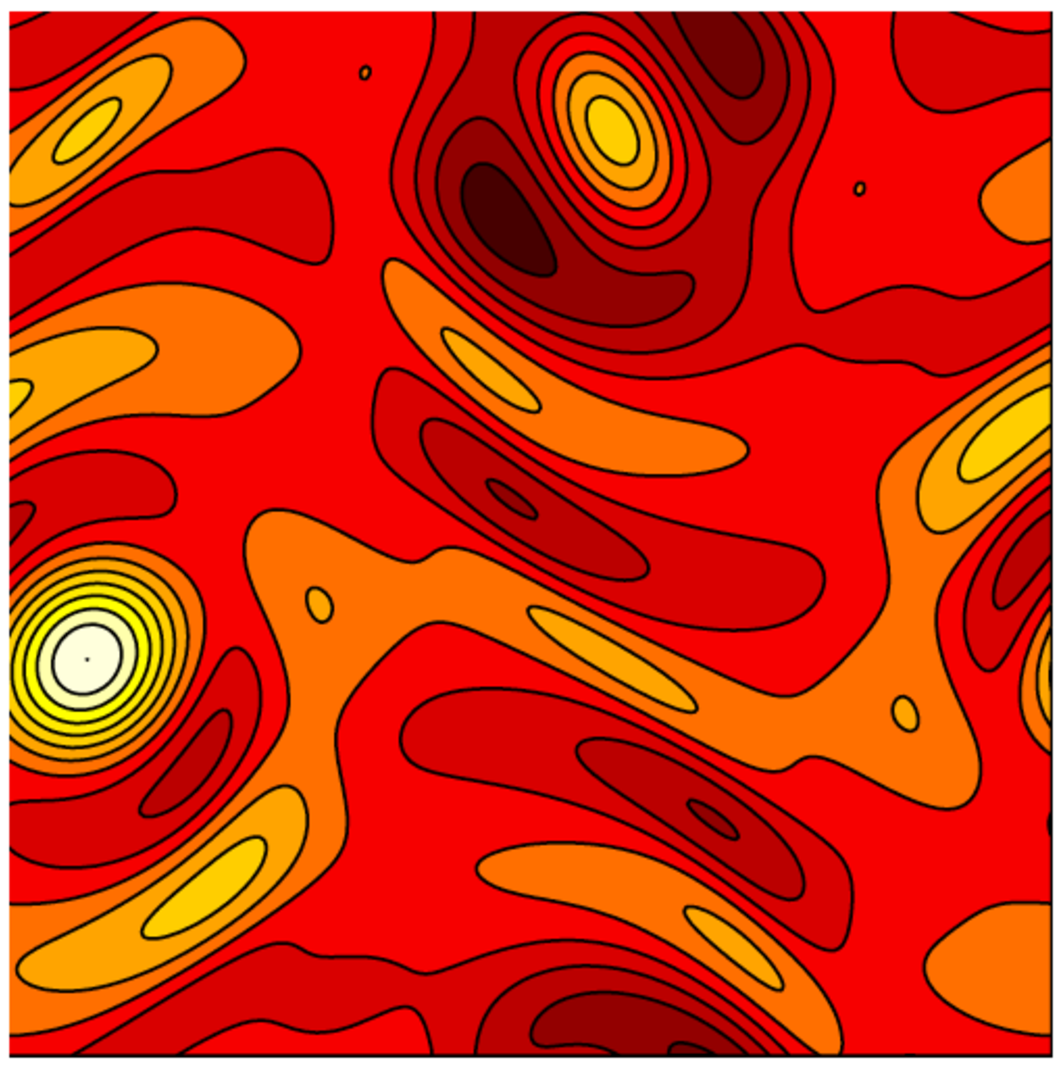
\includegraphics[width=.40\textwidth]{Kol_CK13_E1}
	(b)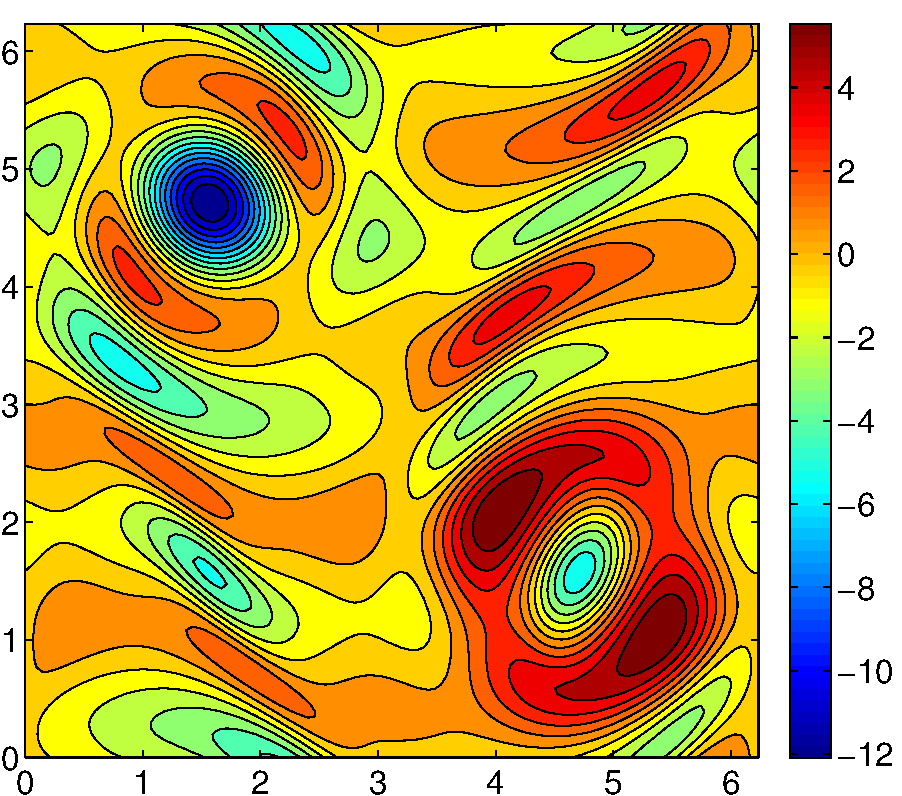
\includegraphics[width=.47\textwidth]{Kol_R40_n128_vort_adj+newton}
	\caption{(a) Equilibrium E1 found by Chandler \& Kerswell, JFM 722 (2013) (b) The
	same equilibrium found by adjoint equation integrated for $4\times 10^4$ time units
	(takes approximately $3$ minutes) plus 7 iterations of Newton-GMRES to decrease the
	$L^2$ error to $5\times 10^{-13}$. Here, $\mbox{Re}=40$. Note that panels (a) and (b)
	appear to be related
	by a shift-and-reflect symmetry.}
	\label{fig:Kol_R40_E1}
\end{figure}
}
	
\MMFpost{2015-02-24}{Playing around with Burgers' equation:
\begin{equation}
	\partial_t u + u\,\partial_x u = \nu\, \partial_x^2 u + f(x,u),
	\label{eq:burger}
\end{equation}
where $x\in \mathbb T=[0,2\pi]$, $t\in\mathbb R^+$ and $f(x,u)$ is some forcing. If the
viscosity $\nu>0$ is large enough the solutions remain smooth for all times.

Some properties:
\begin{enumerate}
\item In the absence of forcing, i.e. $f(x,u)=0$, all solutions converge asymptotically
to the trivial solution $u\equiv 0$.	

\item At the first sight, it appears that the forcing term $f(x,u)=\partial_x u$
produces traveling wave solutions. However as it injects zero average energy in the
system, these solutions decay to $u\equiv 0$ (see \reffig{fig:burger}(a)). The zero
energy input is due to the fact that
$$\int_0^{2\pi} u\,\partial_x u\; dx=0.$$

\item Interestingly, fractional-order forcing
$$f(x,u)=\partial_x^{1/2} u,$$
produces self-sustaining traveling waves (see \reffig{fig:burger}(b)).
\end{enumerate}
\begin{figure}
	\centering
	(a)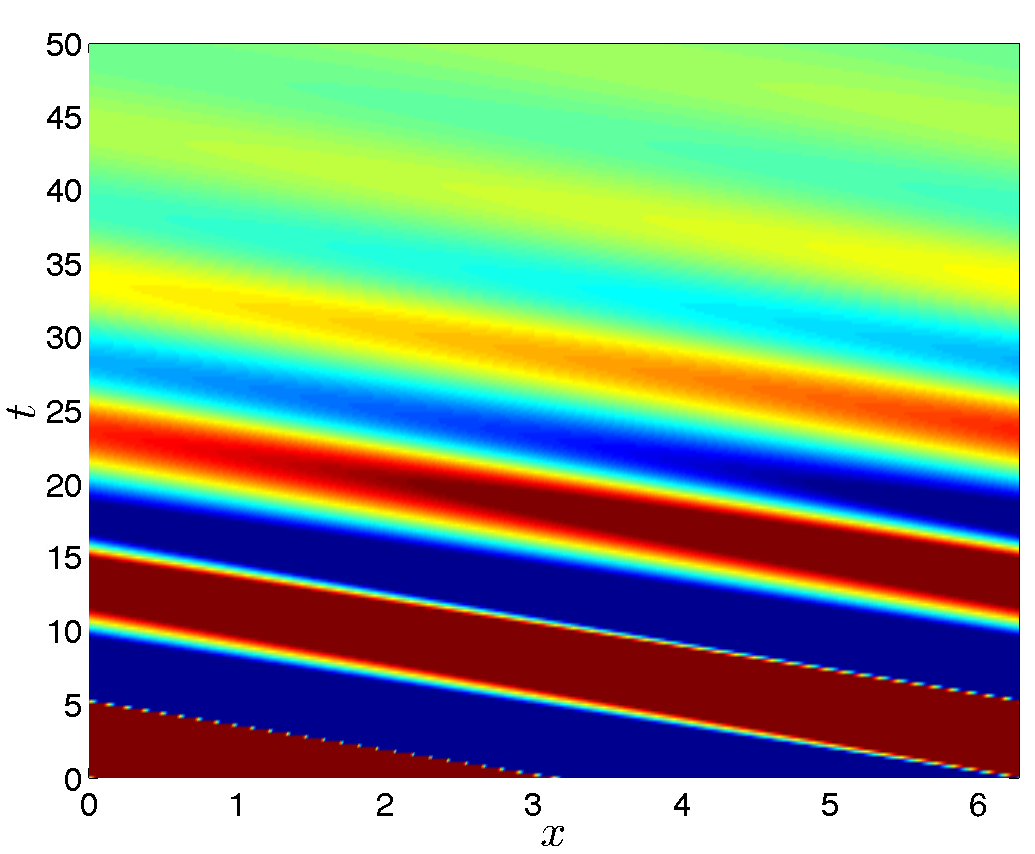
\includegraphics[width=.45\textwidth]{burger_uxForcing}
	(b)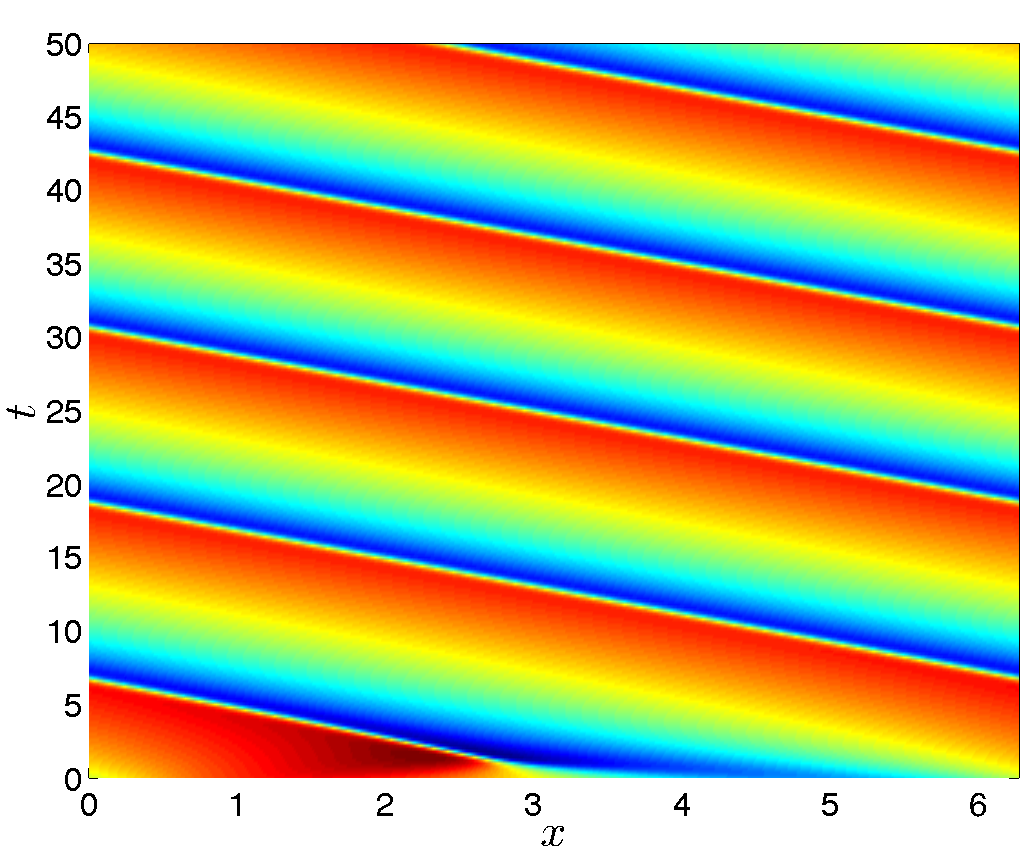
\includegraphics[width=.45\textwidth]{burger_fracForcing}
	\caption{Burgers equation with $\nu = 0.1$. (a)  Forcing $f(x,u)=0.5\,\partial_x u$
	(b) Forcing $f(x,u)=0.5\,\partial_x^{1/2} u$.}
	\label{fig:burger}
\end{figure}
}

    \PCpost{2015-01-24}{
As I'm writing up the {\em Life in extreme dimensions} section of
ChaosBook \texttt{flows.tex}, I have found other interesting references,
for example J. Hopcroft and R. Kannan\rf{HopKan14} and
\HREF{https://www.cs.cmu.edu/~venkatg/teaching/CStheory-infoage/} {Ravi
Kannan}'s course.
One might want to scan through
\HREF{http://sankhya.isical.ac.in/search/64a2/64a2031.pdf} {Wegman and
Solka}\rf{WegSol02} approach to visualizing high-dimensional data.
There is also an interesting mathoverflow.org
\HREF{http://mathoverflow.net/questions/25983/intuitive-crutches-for-higher-dimensional-thinking}
{thread}.
    }

    \PCpost{2014-11-10, 2015-01-11}{                            \inCB
I love it. Flaschka's notes are a very high quality solution set to
\refexer{exer:2vecOrthog} {\em In high dimensions any two vectors are
(nearly) orthogonal} that Sara and I wrote up for Xiong, Burak and
Mohammad, in hope that they would do it. Once one does it, one
understands why {\fFslice} give Predrag ulcers...

If you write it up, please enter the solution into solutions in
\refchap{c-PDEs}. I refer to it in the chapter \texttt{flows.tex} (so far
unwritten) section \emph{Life in extreme dimensions}, and the the new set
of videos for
\\
 \wwwcb{/course1/Course1w1.html}.

Sooner, rather than later I (or some combination of us) should add this
section to \texttt{flows.tex}...
    }


    \MMFpost{2015-01-10}{                            \inCB
I came across the very interesting lecture notes by Hermann Flaschka on
\emph{Some geometry in high-dimensional spaces}. Here is
\HREF{http://math.arizona.edu/~flaschka/Topmatter/527files/concentration.pdf}
{the link}. I'm learning a lot from it and will blog if something
relevant is found.
    }

\MMFpost{2014-12-12}{
Each relative equilibrium of modified perturbed KS has its own domain of attraction. Depending on which domain an initial condition falls in, the solution converges to the corresponding equilibrium. \reffig{fig:modPertKS_L32pi_01} shows that starting from a different initial condition, the modified perturbed KS converges to a different relative equilibrium. To obtain all relative equilibria, we need a smart way to distinguish their domains of attractions approximately.
\begin{figure}
	\centering
	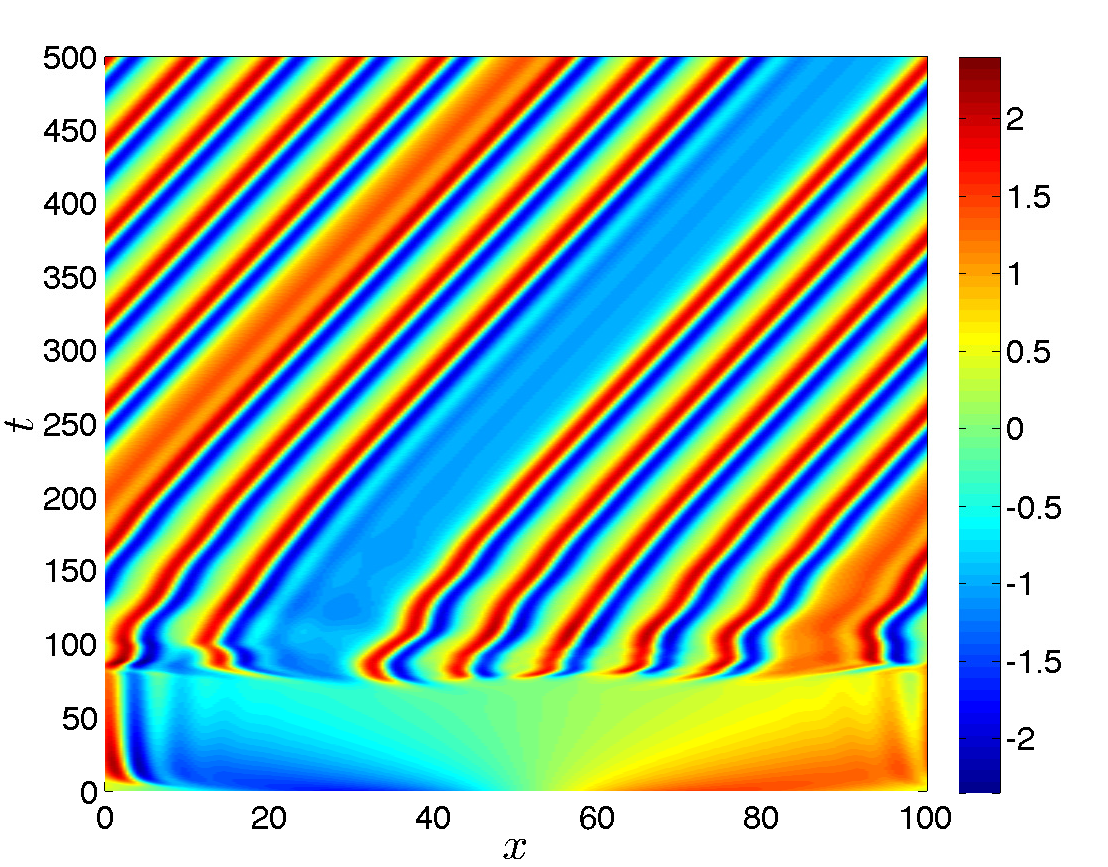
\includegraphics[width=.48\textwidth]{KS_L32pi_icRand_3e0_01}
	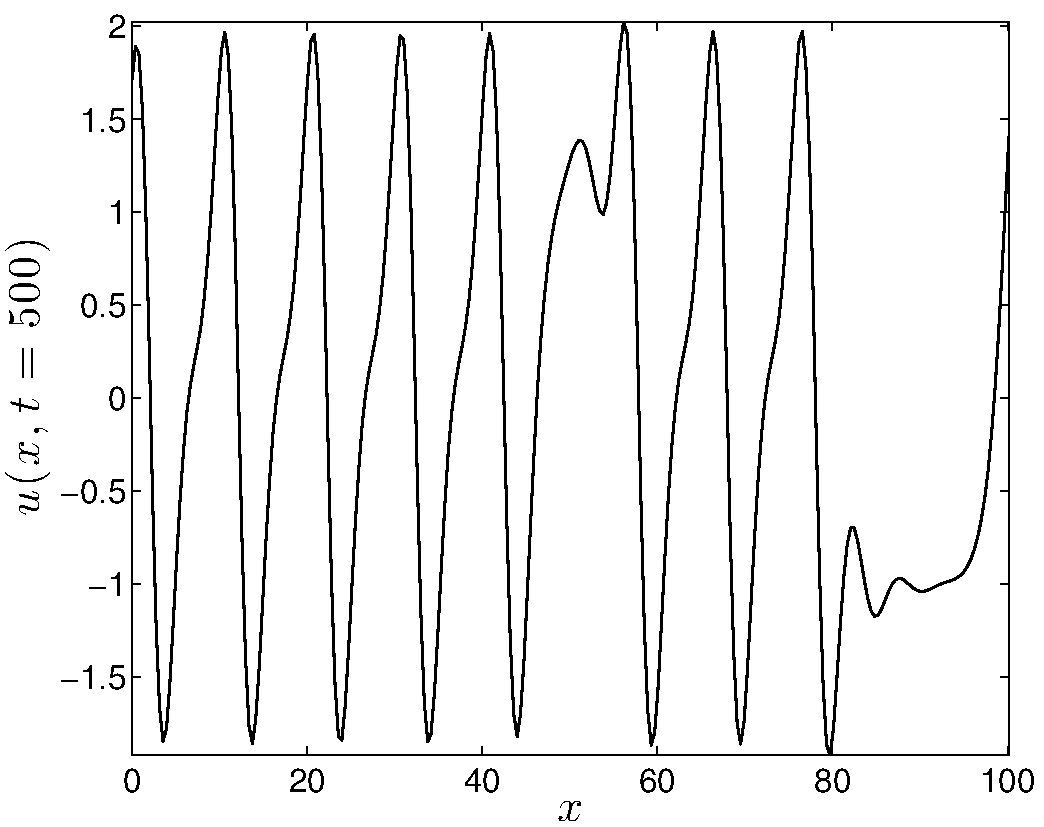
\includegraphics[width=.48\textwidth]{KS_L32pi_icRand_3e0_profile_01}
	\caption{$\tilde L=L/2\pi=16$. Same as the right panel of \reffig{fig:modPertKS_L32pi} starting from a different initial condition.}
	\label{fig:modPertKS_L32pi_01}
\end{figure}
}
	
\MMFpost{2014-12-12}{My guess for the failure of the \emph{perturbed KS} equation \refeq{eq:pertKS} was that in the Fourier space it contains terms up to the order $+k^8$ where $k$ is the wavenumber. This introduces highly unstable modes that the numerical integrator is not able to resolve.
	
The $k^8$-term comes from the fourth-order derivative $-[F(u)]_{xxxx}$ in equation \refeq{eq:pertKS}. So, I decided to neglect this term and solve the \emph{modified perturbed KS} equation:
\begin{equation}
u_t=F_\epsilon(u):=F(u)+\epsilon\{-F(u)u_x-u[F(u)]_x-[F(u)]_{xx} \} ,\quad x\in[0,L].
\label{eq:modPertKS}
\end{equation}

Interestingly, this crude modification seems to work. \reffig{fig:modPertKS_L32pi} compares a solution of KS \refeq{eq:KS} and the solution of the modified perturbed KS \refeq{eq:modPertKS} starting from the {\bf same initial condition} $u(x,0)$. While the solution of KS is turbulent, the solution of the modified perturbed KS converges to a relative equilibrium.

The relative equilibria of perturbed KS should be close to those of KS. To check this, I take the solution of modified perturbed KS at time $t=400$ and use it as initial condition for KS. Figure \ref{fig:modPertKS_L32pi_restart} shows that in fact the relative equilibrium of modified perturbed KS is close to a relative equilibrium of KS.
\begin{figure}
		\centering
		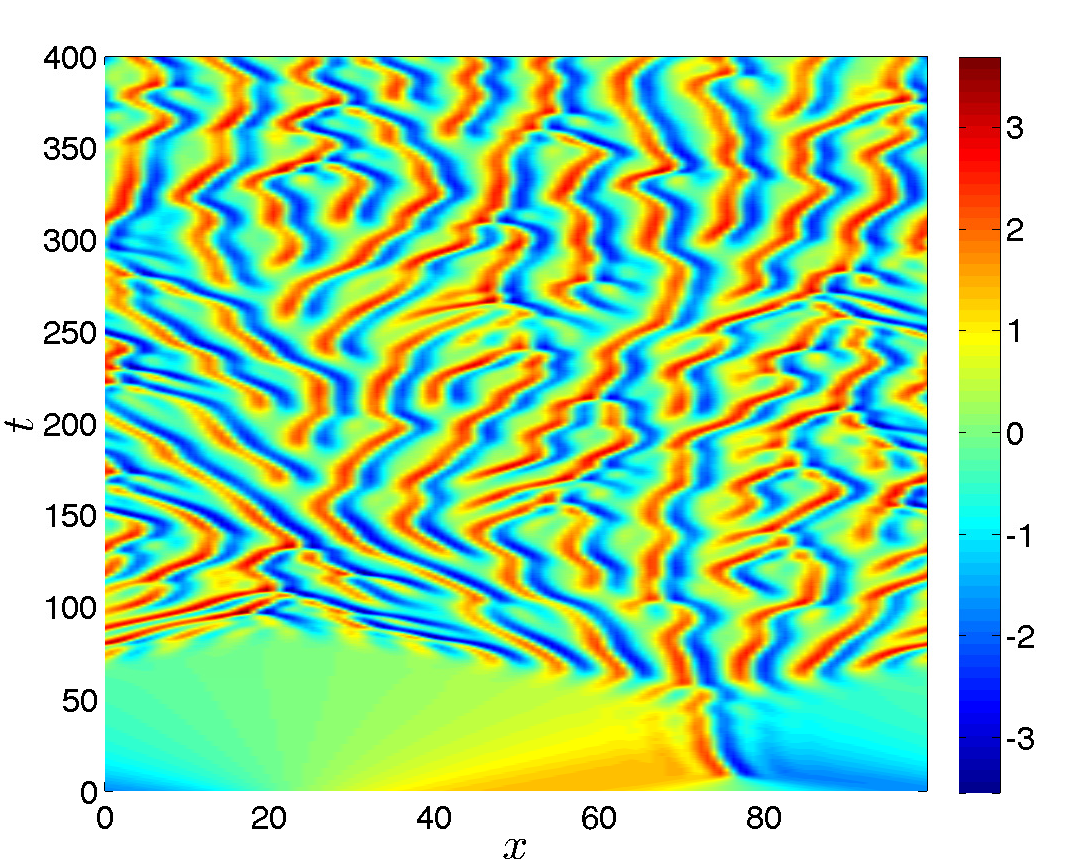
\includegraphics[width=.48\textwidth]{KS_L32pi_icRand_eps0e0}
		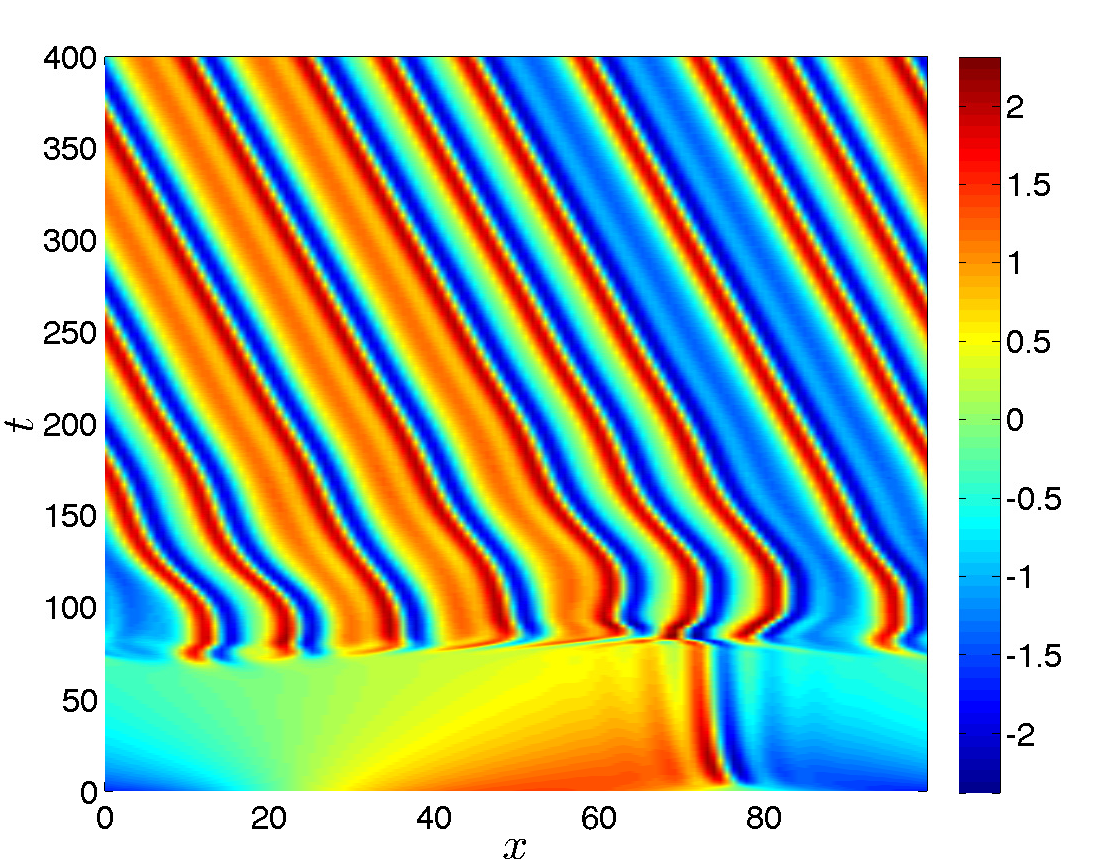
\includegraphics[width=.48\textwidth]{KS_L32pi_icRand_eps3e0}
		\caption{$\tilde L=L/2\pi=16$ (i.e. $L=32\pi$) {\bf Left:} Solution of KS equation \refeq{eq:KS}. {\bf Right:} Solution of modified perturbed KS equation \refeq{eq:modPertKS} with $\epsilon=3$.}
		\label{fig:modPertKS_L32pi}
\end{figure}
%
\begin{figure}[h!]
	\centering
	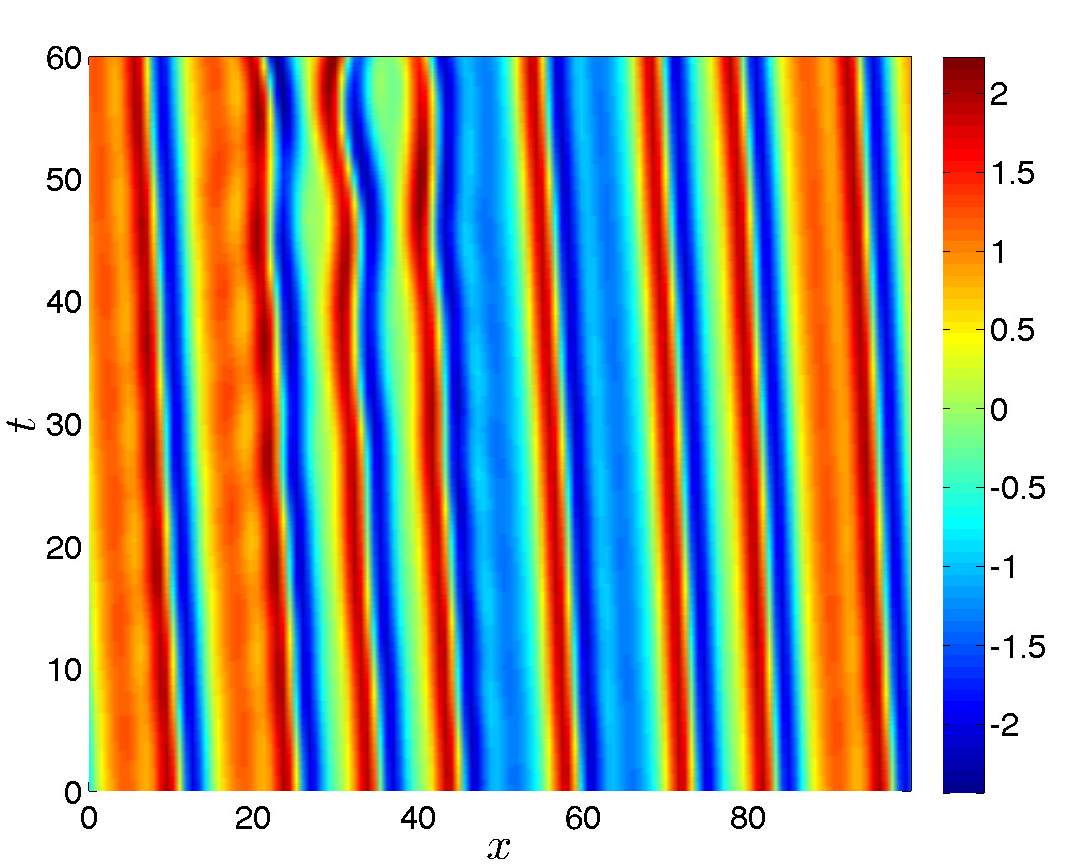
\includegraphics[width=.48\textwidth]{KS_L32pi_icRestart_0e0}
	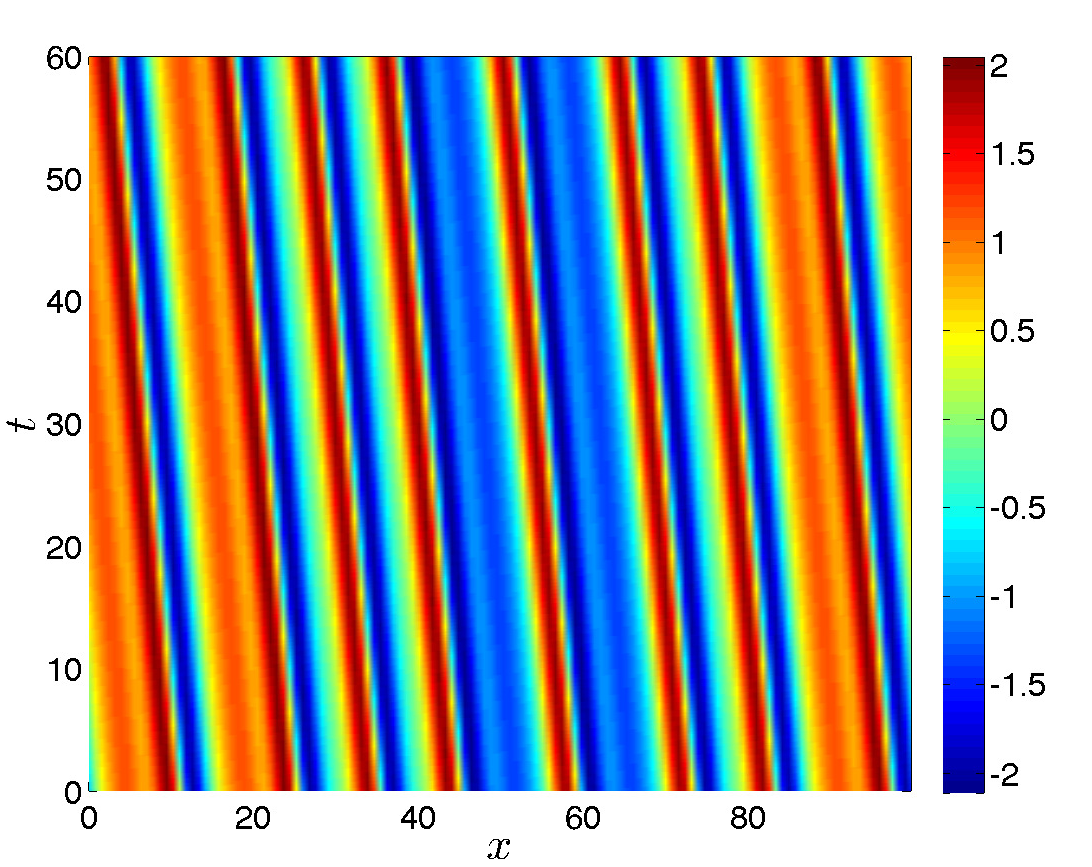
\includegraphics[width=.48\textwidth]{KS_L32pi_icRestart_3e0}
	\caption{$\tilde L=L/2\pi=16$. {\bf Left:} Solution of KS \refeq{eq:KS} starting from $u_0(x)=u(x,t=400)$ where $u(x,t)$ is the solution shown in the right panel of \reffig{fig:modPertKS_L32pi}. The solution follows a relative equilibrium. The instabilities finally take the solution away at around $t=40$. {\bf Right:} The relative equilibrium of modified perturbed KS \refeq{eq:modPertKS} is shown for reference.}
	\label{fig:modPertKS_L32pi_restart}
\end{figure}
}
\MMFpost{2014-12-09}{To Predrag: I tried the ``fast direct method" on KS to converge to its \reqva. I failed! So, here I document what I did. Maybe I'm making a mistake.

Consider the Kuramoto--Sivashinsky (KS) equation with periodic boundary conditions:
\begin{equation}
u_t=F(u):=-uu_x-u_{xx}-u_{xxxx},\quad x\in[0,L].
\label{eq:KS}
\end{equation}
Figure \ref{fig:KS_L32pi} shows a typical solution with $L=32\pi$. (I played around with the length $L$ and tried various sizes, including $L=22$).

By analogy with the finite dimensional case, I add a small ``acceleration term" to KS, i.e., solve
\begin{equation}
u_t=F_\epsilon(u):=F(u)+\epsilon u_{tt},\quad x\in[0,L],\quad 0<\epsilon\ll 1.
\label{eq:pertKS}
\end{equation}
Taking a time derivative of KS, it follows that
$$u_{tt} = -F(u)u_x-u[F(u)]_x-[F(u)]_{xx}-[F(u)]_{xxxx},$$
which coincides with the G\^ ateaux differential of $F$ at $u$ in direction $u_t=F(u)$, that is
$$u_{tt} = dF(u;u_t).$$

I solved \refeq{eq:pertKS} numerically starting from various initial conditions and various parameter values $\epsilon$. And with no luck in converging to a \reqva. Remember that in the case of 2-mode Porter-Knoblock and complex Lorenz, I converged to the \reqva\ starting from arbitrary initial conditions.
\begin{figure}
	\centering
	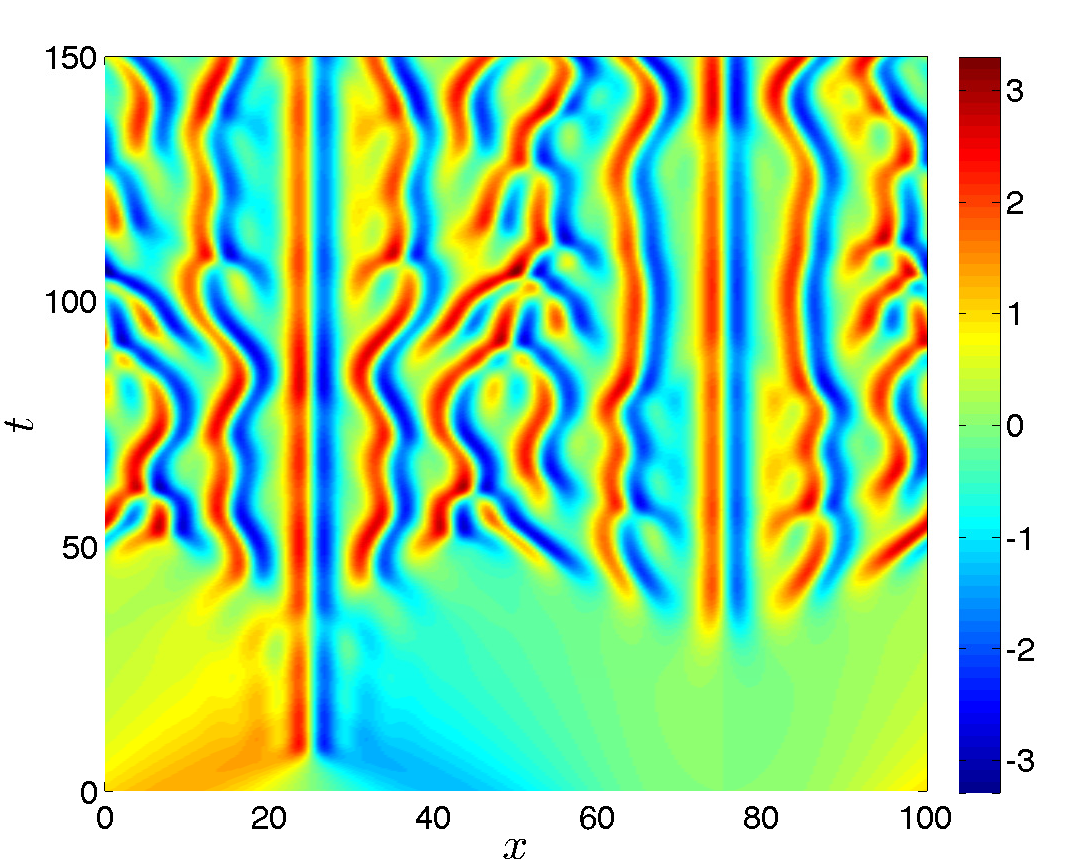
\includegraphics[width=.7\textwidth]{KS_L32pi_ic2}
	\caption{A typical solution of Kuramoto-Sivashinsky equation with domain size $L=32\pi$.}
	\label{fig:KS_L32pi}
\end{figure}
}

\MMFpost{2015-01-14}{Applying the stabilizing vector field \refeq{eq:u} to the Henon map
	\begin{equation*}
	(x,y)\mapsto (1-ax^2+y,by)
	\end{equation*}
	with $a=1.4$ and $b=0.3$. Define $\mathbf x=(x,y)$ and denote the Henon map by $f$: $\mathbf x\mapsto f(\mathbf x)$.
	
	\refFig{fig:henon_stabilizingFlow}(a) shows the convergence of a trajectory of the stabilizing flow $$u(\mathbf x)=-[\nabla v(\mathbf x)]^{-1}v(\mathbf x)$$ to a cycle of order $n=20$. \refFig{fig:henon_stabilizingFlow}(b) shows the evolution of the error
	$$\|\mathbf x(t)-f^n(\mathbf x(t))\|,$$
	with $n=20$ where $\mathbf x(t)$ is a trajectory of $u$ and $\|\cdot\|$ denotes the Euclidean norm on $\mathbb R^2$.
	\begin{figure}
		(a)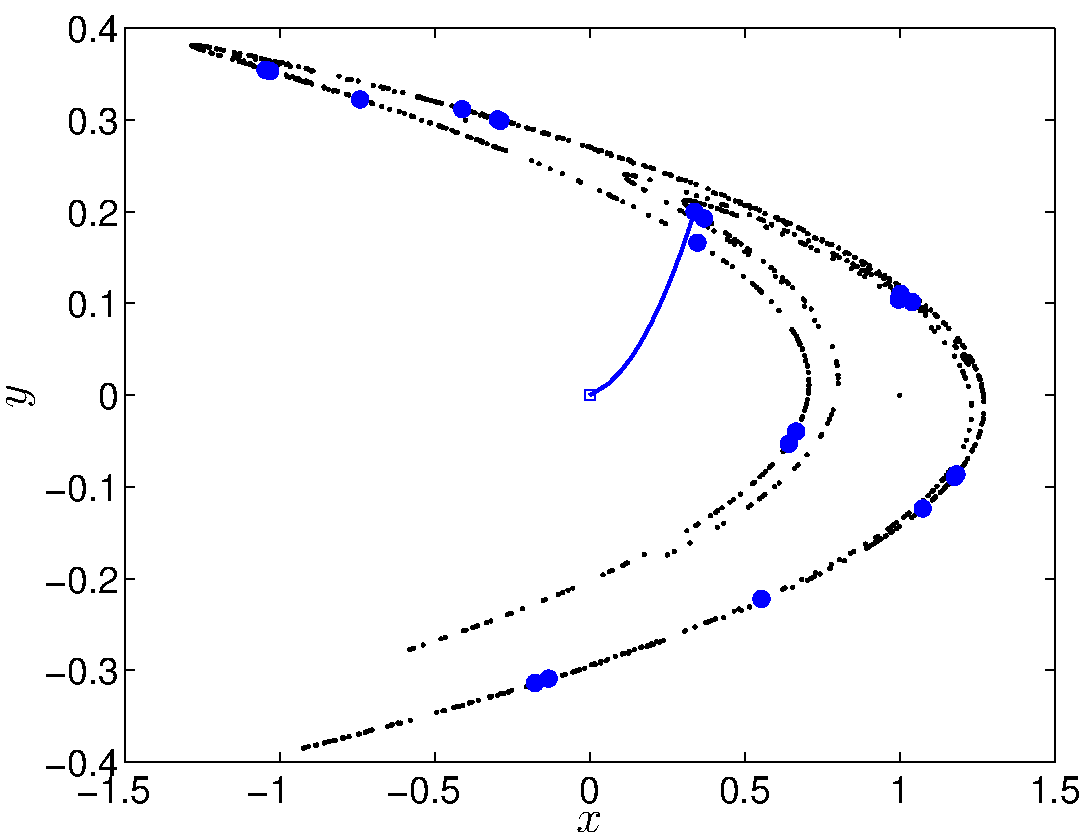
\includegraphics[width=.48\textwidth]{henon_N20_traj}
		(b)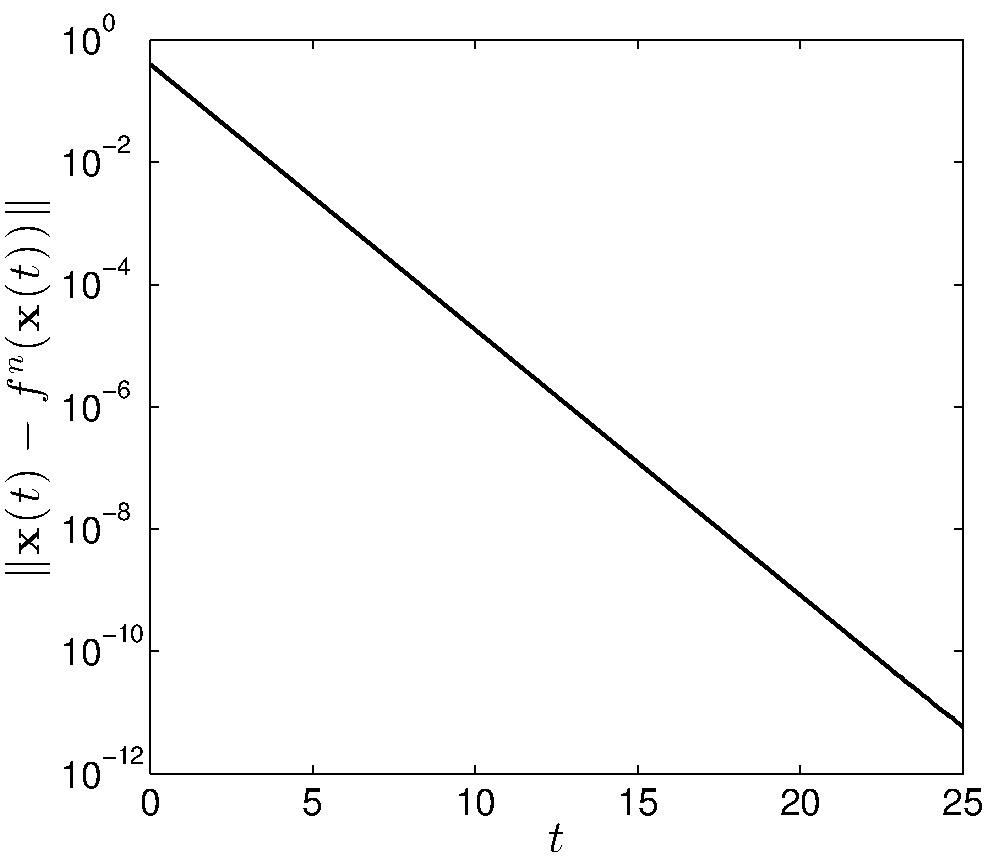
\includegraphics[width=.42\textwidth]{henon_N20_error}
		\caption{(a) An order $20$ cycle of the Henon map: $f^{20}(\mathbf x)=\mathbf x$. The initial condition $(0,0)$ for the stabilizing vector field $u$ is shown by a blue square. The blue curve shows the corresponding trajectory $\mathbf x(t)$. The blue dots show $20$ iterations of the Henon map starting from the end point of the trajectory $\mathbf x(t)$. (b) The evolution of the error $\|\mathbf x(t)-f^n(\mathbf x(t))\|$ with $n=20$. The error decreases monotonically at an exponential rate.}
		\label{fig:henon_stabilizingFlow}
	\end{figure}
}

\MMFpost{2015-01-14}{The vector field \refeq{eq:u} can be derived from an equivalent, norm-dependent formulation:
	
	Consider a given vector field $v:U\rightarrow \mathbb R^m$ where $U\subset\mathbb R^m$. The equilibria, $x\in U$ such that $v(x)=0$, are the minimizers of the functional
	$$\mathcal F(x)=\|v(x)\|^2,$$
	where $\|\cdot\|$ is the Euclidean norm. Let $\delta x\in\mathbb R^m$ and $\|\delta x\|\ll 1$. Then
	$$\mathcal F(x+\delta x)=\mathcal F(x)+2\langle v(x),\nabla v(x)\delta x\rangle +\mathcal O(\|\delta x\|^2).$$
	To ensure that $\mathcal F(x+\delta x)\leq \mathcal F(x)$ for small $\delta x$, it is sufficient to have
	$$\nabla v(x)\delta x=-v(x),$$
	or equivalently
	$$\delta x=-[\nabla v(x)]^{-1}v(x).$$
	Equation \refeq{eq:u} is the infinitesimal version of the above `Newton-Raphson' iteration.
}

\MMFpost{2015-01-13}{The fictitious vector field $u(x)=-\nabla v(x)\, v(x)$ described below can also be used to find fixed points and cycles of maps.
	
	Consider the map $x\mapsto f(x)$ defined over $\mathbb R^m$. For finding fixed points $x=f(x)$, we let $v(x)=x-f(x)$ where $\nabla v(x) = I_m-\nabla f(x)$.
	
	For a cycles of order $n$, where $x=f^n(x)$, we let $v(x)=x-f^n(x)$ and hence
	$$\nabla v(x) = I_m-\nabla f(f^{n-1}(x))\nabla f(f^{n-2}(x))\cdots\nabla f(x).$$
	
	For large $n$, the numerical accuracy can be improved using an idea from Chaos Book. Namely, extend the system by a vector $(x_1,x_2,\cdots,x_n)\in\mathbb R^{n\times m}$ such that $x_2=f(x_1)$, $x_3=f(x_2)$, ..., $x_1=f(x_{n})$, where $x_i\in\mathbb R^m$.
}

	\MMFpost{2014-11-29}{
One more example for the stabilizing flow of equilibria as explained below, i.e., $u =-(\nabla v)^{-1} v$.

Consider the pendulum
\begin{equation}
\dot x_1= x_2,\quad \dot x_2=-\sin(x_1).
\label{eq:pendulum}
\end{equation}
That is $v(x_1,x_2)=(x_2,-\sin(x_1))$. Therefore, we have
$$u(x_1,x_2)=(-\tan(x_1),-x_2).$$

\reffig{fig:pendulum} shows the trajectories of $u$ which take initial conditions to the fixed points of $v$: $x_1=0,\pm\pi$, $x_2=0$.

Note that the equilibria of $v$ all become \emph{stable} equilibria of $u$ with the following domains of attraction:
$$\mbox{Domain of attraction of}\ (0,0) = \{-\pi/2<x_1<\pi/2\}\times \{x_2\in\mathbb R\}$$
$$\mbox{Domain of attraction of}\ (\pi,0) = \{\pi/2<x_1\leq\pi\}\times \{x_2\in\mathbb R\}$$
$$\mbox{Domain of attraction of}\ (-\pi,0) = \{-\pi\leq x_1<-\pi/2\}\times \{x_2\in\mathbb R\}$$

Also, note that $u$ is not defined on $x_1=\pm\pi/2$ since $\nabla v$ is singular on these lines. These singularity lines separate the domains of attraction of the equilibria of $u$.
\begin{figure}[h!]
\centering
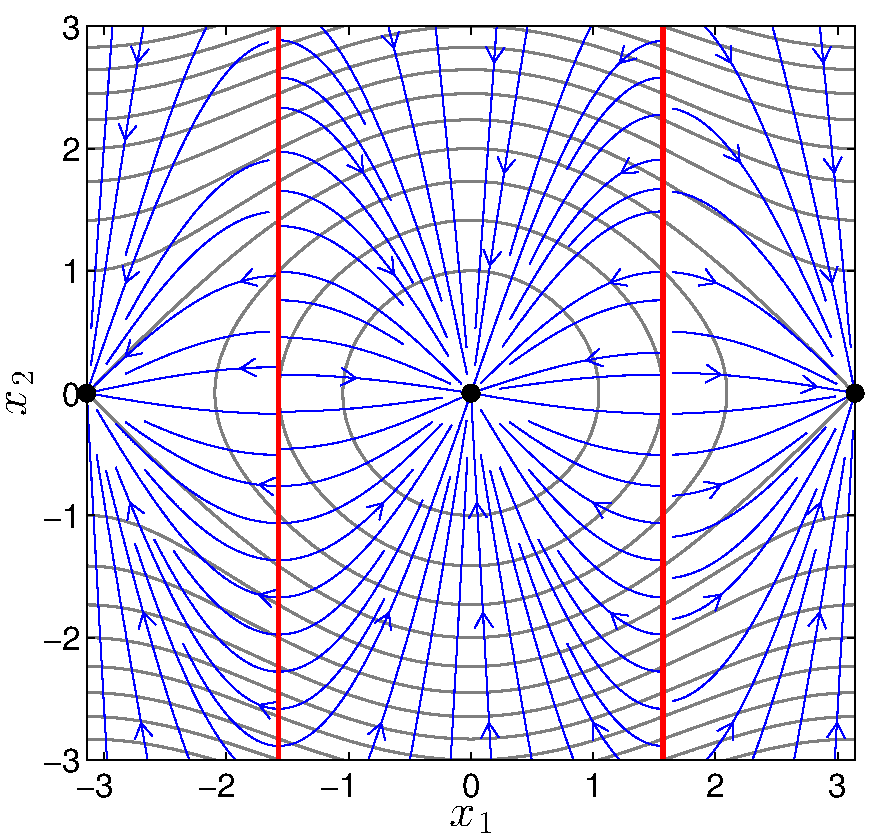
\includegraphics[width=.7\textwidth]{pendulum_stabilizingFlow_02}
\caption{Gray color: Solutions of the pendulum equation \refeq{eq:pendulum}. Black dots: The equilibria $x_1=0,\pm\pi$, $x_2=0$. Blue color: The trajectories of the stabilizing vector field $u$. Red lines: Singularities of $u$ which divide the domains of attraction of the equilibria.}
\label{fig:pendulum}
\end{figure}
}
				
	\MMFpost{2014-11-29}{There are many ways to search for the equilibria of a differential equation
$$\dot x=v(x),\quad x\in\mathbb R^n.$$
They include
\begin{enumerate}
\item Finding the zeros of the algebraic equation $v(x)=0$, using some Newton method.
\item Finding the solutions of $f^t(x)=x$ for all $t$, where $f^t$ is the solution map of the differential equation. This is sometimes done by finding the minimizers of $\|f^t(x)-x\|^2$ for all $t$. This assumes a norm $\|\cdot\|$ and then uses Newton iterations or Newton descent method (introducing a fictitious time $\tau$).
\end{enumerate}

Here is a third method which combines the two approaches above but does NOT use a norm. The problem can be formulated as follows: Find a dynamical system $g^\tau$ such that $\lim_{\tau\rightarrow\infty}v(g^\tau(x))=0$ for all $x$.

To find such a flow $g^\tau$, define
$$\phi(\tau;x)=v(g^\tau(x)),$$
for an arbitrary $x\in\mathbb R^n$. Constrain $g^\tau$ such that $\lim_{\tau\rightarrow\infty}\phi(\tau;x)=0$. This constraint can be imposed in several ways. One is to require $\phi(\tau;x)$ to satisfy the following ODE:
\begin{equation}
\partial_\tau\phi(\tau;x)=-\phi(\tau;x),
\label{eq:const}
\end{equation}
whose solutions are $\phi(\tau;x)=\phi(0;x)\exp(-\tau)=v(x)\exp(-\tau)$.

Now, from definition of $\phi$ we have $\partial_\tau\phi = \nabla v(g^\tau(x))\partial_\tau g^\tau(x)$. If $u$ is the infinitesimal generator of $g^\tau$, i.e. $\partial_\tau g^\tau(x)=u(g^\tau(x))$, we get $\partial_\tau\phi=\nabla v(g^\tau(x))u(g^\tau(x))$. This, together with constraint \refeq{eq:const}, implies
$$ \nabla v(y)u(y)=-v(y),\quad y=g^\tau(x).$$
If $\nabla v$ is (almost everywhere) invertible, $u$ is explicitly defined in terms of $v$ as
\begin{equation}
u =-(\nabla v)^{-1} v.
\label{eq:u}
\end{equation}

{\bf Examples:} Consider the linear saddle
$$ \dot x_1 = x_1,\quad \dot x_2=-x_2,\quad x_1,x_2\in \mathbb R$$
and the harmonic oscillator
$$\dot x_1 =x_2,\quad \dot x_2=-x_1,\quad x_1,x_2\in \mathbb R.$$
The first equation has a hyperbolic fixed point at the origin while the second equation has a center fixed point at the origin. Using \refeq{eq:u}, the auxiliary vector field $u$ for both the saddle and the harmonic oscillator is
$$u(x_1,x_2)=(-x_1,-x_2),$$
whose flow $g^\tau$ takes any initial condition $x$ to the equilibrium at the origin, exponentially fast.

In fact, for any smooth linear flow $v(\mathbf x)=A\mathbf x$ with $\mathbf x\in \mathbb R^n$, we have $u(\mathbf x)=-A^{-1} v=-A^{-1}A\mathbf x= -\mathbf x$. The flow of $\dot{\mathbf x}=u(\mathbf x):=-\mathbf x$ takes any initial condition to the fixed point $\mathbf x=0$.
}

    \PCpost{2014-11-22}{

{\bf A fast explicit method for computing unstable invariant
        solutions of high-dimensional dynamical systems}

{\bf Desiderata}:
Find a method that determines time-invariant unstable solutions (or their
neighborhoods) of a given dynamical system without imposing any
extraneous norm on the \statesp\ of the system. By that one means a
method other than a Newton method or optimization methods that minimize
squares of errors computed with an externally imposed norm, not intrinsic
to dynamics.

{\bf Proposal}:
Modify the flow in the neighborhood of an unstable invariant set with terms
quadratic in the linearized stability exponents, parametrized
by $M$ small parameters $\epsilon_j$, one for each distinct positive real
part \eigRe[j] of a stability exponent
$\eigExp[j]=\eigRe[j]\pm\eigIm[j]$, in such a way that all stability
exponents of the modified flow are contracting, and the flow converges to
an $\epsilon$-nearby invariant set.


{\bf Discussion}:
In common iterative schemes or differential equations set up to converge
to desired invariant sets, one always (?) introduces an extra fictitious
time (or the Newton iteration number), see ChaosBook.tex Sect.~29.1
\HREF{http://www.streamsound.dk/book1/chaos/chaos.html\#613/z}
{\emph{Fictitious time relaxation}} and
\refrefs{CvitLanCrete02,lanVar1,LCC06,Lan:Thesis}. The novelty here is
that the equations of motion themselves are modified, with no
introduction of a fictitious time, and without introducing a norm to
measure the distance to the desired solution. Only linear stability and
directional (Jacobi) derivatives are used.

I think the essence of Mohammad's approach is not in using curvature of
trajectories, but in modifying the flow by adding to it terms quadratic in
eigenvalues of the {\stabmat} {\Mvar} in such a way that the modified
flow converges to a  nearby stable invariant set. Maybe you can think of it
as follows:

(text clipped from ChaosBook.tex Sect.~4.4
\HREF{http://www.streamsound.dk/book1/chaos/chaos.html\#102/z}
{\emph{Stability of flows}}):

The finite time \jacobianM\ $\jMps^\zeit$ is related to the {\stabmat}
{\Mvar} by the formal integral along a trajectory,
\beq
\jMps^\zeit_{ij}(\xInit)
= \left[ {\bf T} e^{ \int_0^\zeit d\tau \Mvar (\ssp(\tau)) } \right]_{ij}
\,,
\label{hodes}
\eeq
where ${\bf T}$ stands for time-ordered integration, {defined} as
the continuum limit of successive multiplications
\beq
\jMps^\zeit =
\lim_{m \to \infty}\prod_{n=m}^1
\left(\matId + \delta t \Mvar(\ssp_n) \right)
\ee{Jprod1}
For nonlinear dynamical
systems, the local rate of neighborhood distortion $\Mvar(\ssp)$
depends on where we are along the trajectory. The linearized
neighborhood is deformed along the flow, and the $m$
discrete time-step approximation to $\jMps^\zeit$ is therefore given
by the above product,
where $\delta \zeit = {(t-t_0)/ m}$, and $\ssp_n=\ssp(t_0+n\delta \zeit)$.
Indexing of the products indicates that the successive infinitesimal
deformation are applied by multiplying from the left.

For convenience, set $\ssp_0 \to \ssp$, expand \refeq{Jprod1} to order
$\delta t^2$,
\bea
\jMps^{2\delta t}(\ssp) &=&
\matId
+ \delta t  \left(\Mvar(\ssp) + \Mvar(\ssp_1)\right)
+ \, \delta \zeit^2 \Mvar(\ssp)^2 + O(\delta \zeit^3)
    \continue
    &=&
\matId
+ 2 \delta \zeit \, \Mvar(\ssp)
    \ceq
+ \delta \zeit^2 \left( (\vel(\ssp)\cdot \nabla)\Mvar(\ssp)
                 + \Mvar(\ssp)^2\right) + O(\delta \zeit^3)
\label{Jprod2}
\eea
replace $\delta \zeit^2 \to \epsilon\delta t$, modify the original
flow accordingly, and use $\epsilon$ to manipulate local stability.

Dimensionally, $\epsilon$ is time (a decay rate toward the \eqv? see
\refeq{stabExpEpsilon}), so one
might consider non-dimensionalizing it.

If looking for an \eqv, on the \eqv\ $\ssp_\stagn$ of the original flow
the pesky `curvature' term $(\vel(\ssp)\cdot \nabla)\Mvar(\ssp)$
vanishes.

{\bf Marginal stability exponents} have to be removed. For \reqva\ this
is achieved by studying eigenvalues of $(\Mvar-\velRel\cdot\Lg)$, see
\refeq{ReqvMargEig}. For \po s this is achieved by any local \Poincare
section, and for \rpo s and hyperbolic $N$-tori
by any (local or global) symmetry reduction
together with any local \Poincare section.

{\bf A single real unstable eigen-direction case}.
If the $\ssp_\stagn$ has an unstable eigenvector
$\jEigvec[j](\ssp_\stagn)$ with a real unstable stability exponent
$\eigExp[j]>0$, at a nearby $\ssp$ they will both pick up terms of order
$\delta \zeit$. Perhaps one can compute the corresponding eigenvector
$\jEigvec[j](\ssp,\delta \zeit)$ at the guess point $\ssp$ and use
the $(\epsilon<0)$-modified real stability exponent $\eigExp[j]+\epsilon
(\eigExp[j])^2$ to reverse flow along 1\dmn\
$\jEigvec[j](\ssp_\stagn,\delta \zeit)$ to now go towards the
$\epsilon$-nearby \eqv\ $\ssp_{\stagn,\epsilon}$.

{\bf A complex pair, 2\dmn\ unstable eigen-plane case}. See below.

{\bf A finite number of expanding directions}.
{\stabmat} {\Mvar} can be brought to a pimply upper-triangular form (a
pimple for each complex pair or other subspace with a single real part of
the stability exponent\rf{DingCvit14}). The unstable flow can be
`reversed' by a range of values for $\epsilon_i$ parameters, one for each
of projections on 1, 2, m\dmn\ subspaces of spanned by sets the
degenerate eigenvectors of the $\epsilon_i$-distorted flow.
    }

	\PCpost{2014-11-22}{
If $ v(x)$ is autonomous, not time dependent, and
\[
a(\ssp)= \frac{d \vel(\ssp)}{d \zeit}
   = \nabla \vel(\ssp)\vel(\ssp) = \Mvar(\ssp)\vel(\ssp)
\]
is the `acceleration', maybe we should double the number of coordinates
to $[y,u]$, $y=\ssp-\epsilon \vel$, and integrate the pair of first
order ODEs,
\bea
{\dot y}_j(\zeit) &=& \vel(y,u)_j
    \continue
{\dot u}_j(\zeit)
 &=& \frac{d \vel_j}{d \ssp_k}\,\vel(y,u)_k
  = \Mvar(y,u)_{jk}\,\vel(y,u)_k
\,,
\eea
from initial condition $[y(0),u(0)]= [\ssp(0),\vel(\ssp(0))]$. Not sure
all this makes sense: it puts \eqv\ at the origin, which cannot be right.
    }


	\PCpost{2014-11-22}{
For \cLe\ unstable \eqv\ at the origin $\lambda_5=-2.67$ presumably has
$z$-axis as its eigenvector. It is an invariant subspace, no need to
discuss it further. I am not sure about your two complex eigenvalue pairs
$\eigExp[1,2]$ and $\eigExp[3,4]$. Remember that they have to be computed
in the symmetry-\reducedsp, as eigenvalues of $(\Mvar-\velRel\cdot\Lg)$,
see \refeq{ReqvMargEig}. We have computed them zillion places, I just
cannot remember off the bat where: ChaosBook? Siminos thesis? Siminos or
Froehlich blogs? \refrefs{SiCvi10,FrCv11}? I seem to vaguely remember one
of them being real, but am not sure. If so,  $(\epsilon<0)$-modified real
stability exponent of my post above would be the right thing. If you have
only one unstable direction (or complex pair) being sloppy about the
choice of contracting direction is OK.
    }

	\MMFpost{2014-11-20}{To Predrag:
Following our discussion today-- \cLe\ has an unstable
{\eqv} at the origin. I have not been able to converge to it for any
$\epsilon>0$ using $v_\epsilon(x)=v(x)+\epsilon (\nabla v(x)) v(x)$. The
eigenvalues of the {\stabmat} {\Mvar} at the origin are:
\[
  \lambda_{1,2}=11.83\pm i 0.063,\quad
  \lambda_{3,4}=-22.83\pm i 0.037,\quad \lambda_5=-2.67
  \,.
\]
	That is $S^+_<\neq\emptyset$; hence condition 1 of the theorem below
is violated.
	
However, for $\epsilon<0$, I do converge to the origin which is good. So,
maybe we need to check both positive and negative $\epsilon$.
}

	\MMFpost{2014-11-18}{ Here is what I have so far. I do it for {\eqv} but a
similar result holds for relative {\eqv} after symmetry reduction. Looking forward
to your opinions/suggestions...

Consider the differential equation $\dot x=v(x)$ on $\mathbb R^n$ which has a fixed point
$x_0$, i.e., $v(x_0)=0$. Then $x_0$ is also a fixed point of the perturbed equation
$\dot x = v_\epsilon(x)$ where $v_\epsilon(x)=v(x)+\epsilon a(x)$ with
$a(x)=\nabla v(x)v(x)$.

Linear stability matrix: Let $A:=\nabla v(x_0)$ and $A_\epsilon:=\nabla v_\epsilon (x_0)$.
For any $x\in\mathbb R^n$, we have
$$ \nabla v_\epsilon(x) = \nabla v(x) + \epsilon [\nabla v(x)]^2 + \epsilon[v(x)\cdot \nabla] \nabla v(x).$$
Substituting $x=x_0$ and using $v(x_0)=0$, we get
$$ A_\epsilon = A + \epsilon A^2$$

Assume $A$ has $n$ distinct eigenvalues
$\lambda_k=\mu_k\pm i\omega_k\in\mathbb C$ (w.l.o.g., let $\omega_k\geq0$). Then there is
a basis in which $A$ is block diagonal with blocks
\begin{equation}
\begin{pmatrix}
\mu_k & -\omega_k \\
\omega_k & \mu_k
\end{pmatrix}.
\end{equation}
The block is a $1\times 1$ scalar matrix for real eigenvalues $\lambda_j=\mu_j$.

In the same basis, $A_\epsilon$ is also block diagonal with blocks
\begin{equation}
\begin{pmatrix}
\mu_k+\epsilon(\mu_k^2-\omega_k^2) & -\omega_k(1+2\epsilon\mu_k) \\
\omega_k(1+2\epsilon\mu_k) & \mu_k+\epsilon(\mu_k^2-\omega_k^2)
\end{pmatrix}.
\end{equation}
Therefore, the real parts of the eigenvalues of $A_\epsilon$ are
\beq
\mu_k+\epsilon(\mu_k^2-\omega_k^2)
\,.
\ee{stabExpEpsilon}
For the point $x_0$ to be a stable fixed point of $\dot x=v_\epsilon(x)$,
we need all the above numbers to be negative.

{\bf Notation:} For determining the conditions of stability of $x_0$, the following
notation will become handy. Let $\{1,2,\cdots,n\}=S^+\cup S^-$ where
$$S^+=\{1\leq k\leq n\ |\ \mu_k\geq 0\},$$
$$S^-=\{1\leq k\leq n\ |\ \mu_k< 0\}.$$
Further split $S^+$ as $S^+=S^+_>\cup S^+_<$ where
$$S^+_>=\{k\in S^+\ |\ \omega_k>\mu_k\},$$
$$S^+_<=\{k\in S^+\ |\ \omega_k\leq\mu_k\}.$$
Similarly split $S^-$ as $S^-=S^-_>\cup S^-_<$ where
$$S^-_>=\{k\in S^-\ |\ \omega_k\geq|\mu_k|\},$$
$$S^-_<=\{k\in S^-\ |\ \omega_k<|\mu_k|\}.$$

With a little algebra, one arrives at the following result.

{\bf Lemma:}
The inequalities $\mu_k+\epsilon(\mu_k^2-\omega_k^2)<0$ are satisfied for all
$1\leq k\leq n$, if and only if,
\begin{enumerate}
	\item $S^+_< = \emptyset$ and
	\item $\epsilon>0$ satisfies
	$$\max_{k\in S^+_>} \frac{\mu_k}{\omega_k^2-\mu_k^2}<\epsilon<\min_{k\in S^-_<} \frac{-\mu_k}{\mu_k^2-\omega_k^2}.$$
\end{enumerate}

All put together, we get the following result for stabilizability of an unstable
{\eqv}:

{\bf Theorem:} Let $v(x_0)=0$ and $\nabla v(x_0)$ have distinct eigenvalues
$\mu_k\pm i\omega_k$ satisfying
\begin{enumerate}
	\item $S^+_< = \emptyset$ and
	\item $\max_{k\in S^+_>} \frac{\mu_k}{\omega_k^2-\mu_k^2}<\min_{k\in S^-_<} \frac{-\mu_k}{\mu_k^2-\omega_k^2}.$
\end{enumerate}

Then for any $\epsilon$ such that $$\max_{k\in S^+_>}
\frac{\mu_k}{\omega_k^2-\mu_k^2}<\epsilon<\min_{k\in S^-_<}
\frac{-\mu_k}{\mu_k^2-\omega_k^2},$$ the point $x_0$ is an asymptotically
stable {\eqv} of $\dot x=v(x)+\epsilon\nabla v(x) v(x)$.
}

\MMFpost{2014-11-18}{
I agree continuous symmetry is not essential; I was actually motivated by
observing that it works for elliptic fixed points.
}

    \PCpost{2014-11-17}{
I think continuous symmetry is not the essential part of your algorithm,
and if you subtract from the {\stabmat} {\Mvar} the other part of the
Jacobi derivative, you will essentially work in the symmetry-reduced
\statesp.

Now, about \po s. Suppose you make a guess at one by placing your guess
loop $L$ into the \statesp. At every point $\ssp\in L$ there are two
vectors - the dynamical velocity field $\vel(\ssp)$ and the tangent of
your loop $t(\ssp)$. Maybe you can construct the new flow by subtracting
the Jacobi derivative of the two, and that will move all points on your
guess loops toward the true \po? On any \po\ this Jacobi derivative vanishes.

Whatever you do, do not take the square of this local Jacobi derivative,
as that requires a (here unwelcome) norm.
    }



    \PCpost{2014-11-17}{
That settles is.

Curious: if in \reffig{fig:stabCmplxLorenz_hilbertBases})\,(a) you use
the same units on two axes (plot this on a square of size 400$\times$400),
does spiral look isotropic, rather than squashed?

Do you know what the new stability exponents are? My guess would be that
the real part has no obvious relation to the original, unstable one
(perhaps has a linear or square root dependence on small $\epsilon$'s?),
but that the imaginary part is the same as for the original {\eqv},
up to $O(\epsilon)$. I'm guessing this as think your method makes a
weekly positive real part $\eigRe{}$, but the imaginary part $\pm
\eigIm{}$ is far of the real axis and it does not shift much.
    }

    \MMFpost{2014-11-17}{
I liked the Hopf bifurcation idea. But it seems that the trajectory of
the perturbed system does really converge to a point after symmetry
reduction. Here is some evidence for complex Lorenz. I calculate the
trajectory of the perturbed system in the Hilbert polynomial bases,
$(u_1,u_2,u_3,u_4,u_5)$ as given in \rf{SiCvi10}. I plot the $(u_1,u_2)$
projection below, indicating the spiral towards a point (see
\reffig{fig:stabCmplxLorenz_hilbertBases}). Similar observation holds for
other projections (not presented here).

Could there be a tiny circle?! To check this, I also plot $u_1(t)$ and
$u_5(t)$ and observe that they converge to a constant as $t$ increases (I
zoomed in on my screen, they are really constant lines). Same is true for
other $u_k(t)$.
    }
\begin{figure}
	\centering
	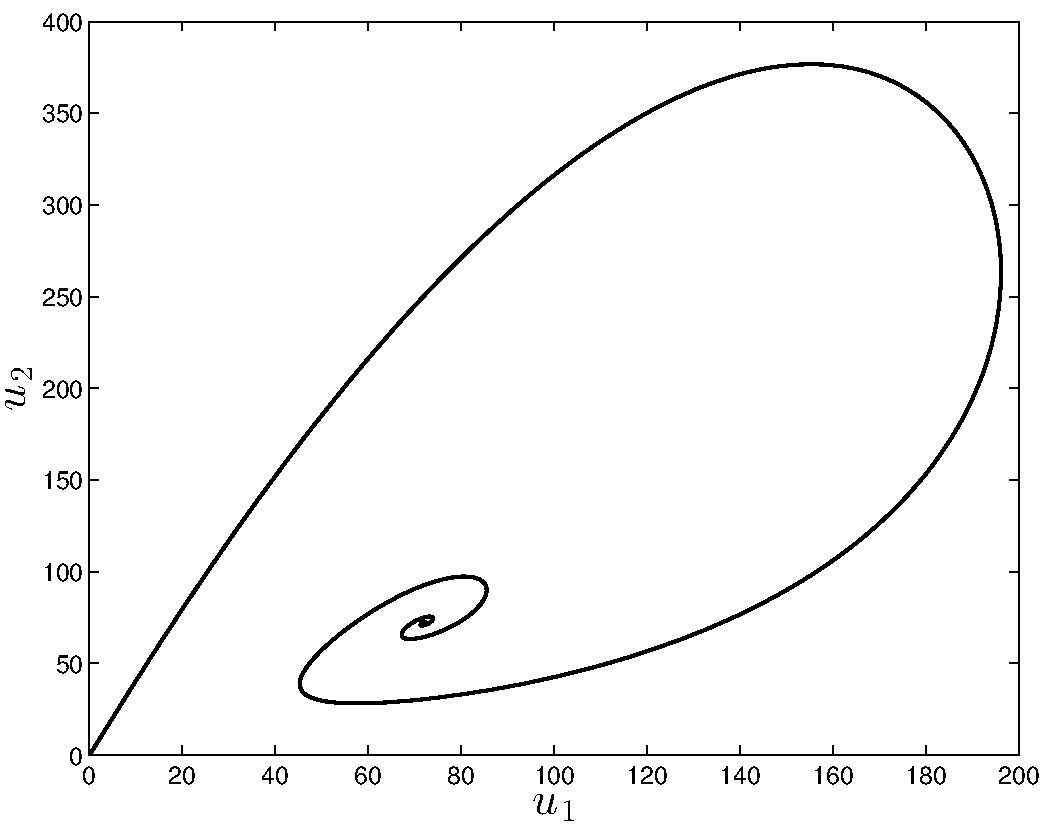
\includegraphics[width=.6\textwidth]{u1vu2_stab_cmlxLorenz.pdf}\\
	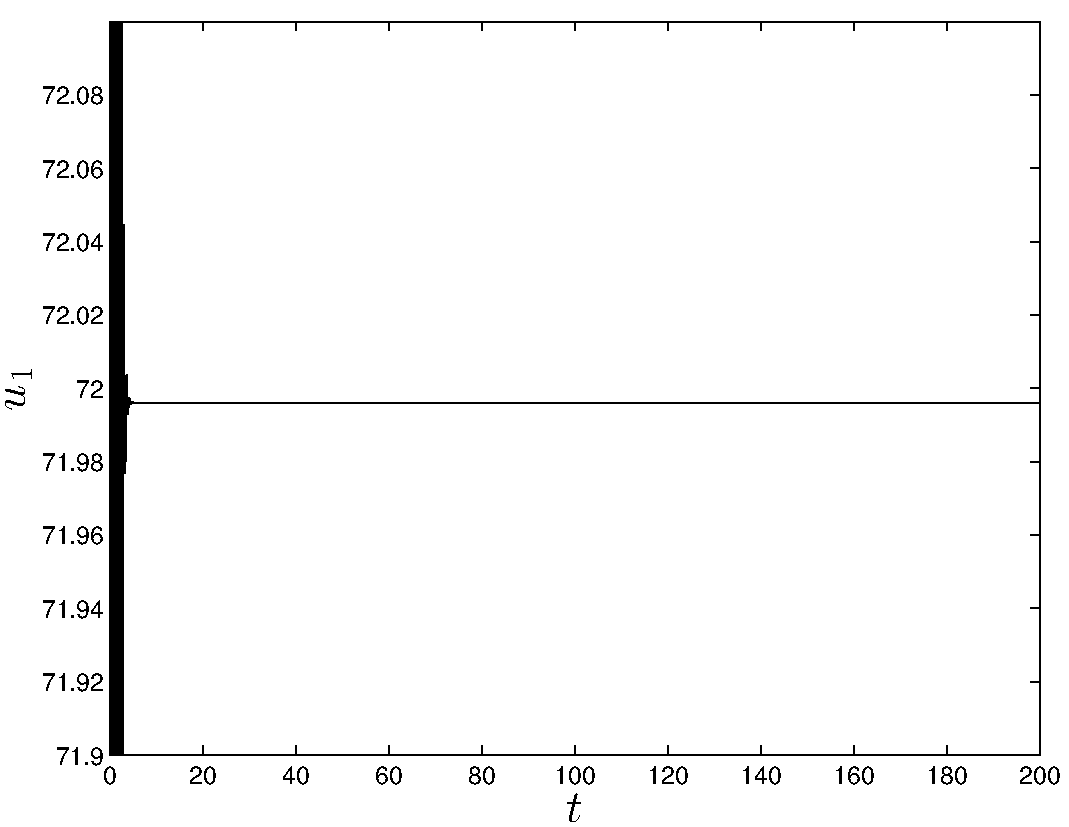
\includegraphics[width=.45\textwidth]{u1vt_stab_cmplxLorenz.pdf}
	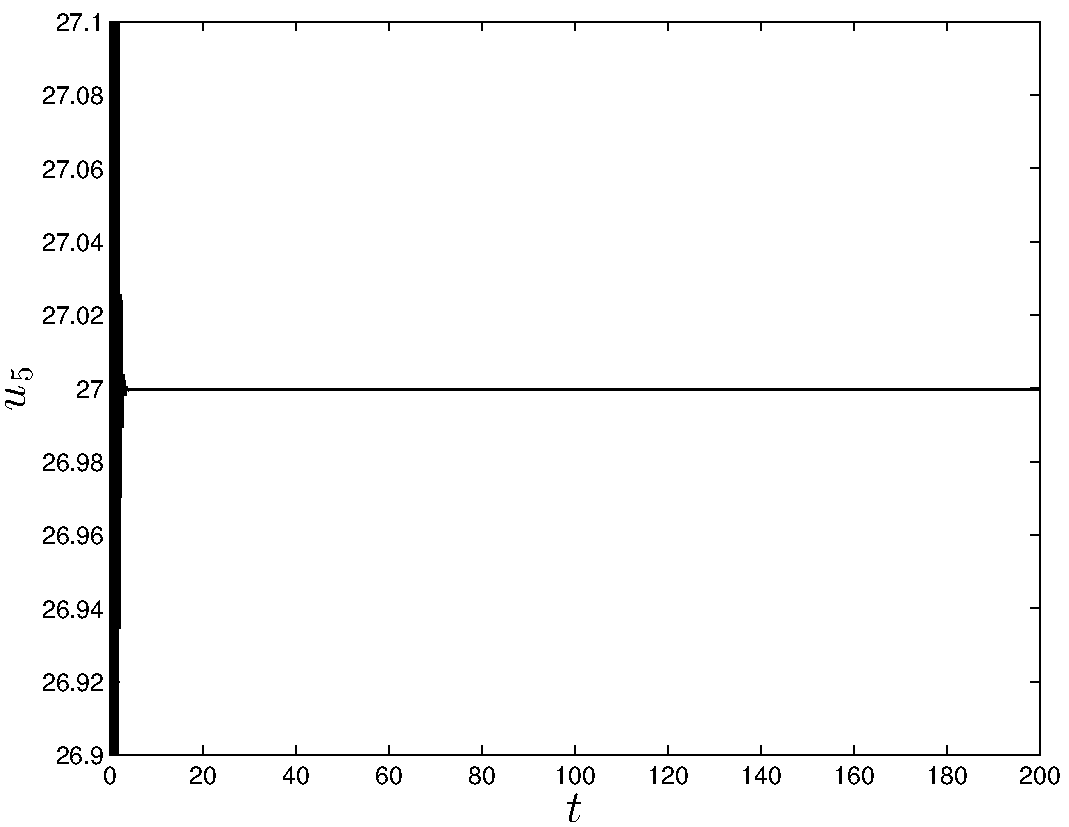
\includegraphics[width=.45\textwidth]{u5vt_stab_cmplxLorenz.pdf}
	\caption{A trajectory of the ``stabilized" complex Lorenz plotted in the Hilbert polynomial basis.}
	\label{fig:stabCmplxLorenz_hilbertBases}
\end{figure}


    \MMFpost{2014-11-16} {
I have done some further analysis that shows that once
you have a (relative) {\eqv} with complex conjugate eigenvalues which satisfy a
a particular condition (similar to spectral gap), the added acceleration
turns it into a stable {\eqv}. This seems in agreement with your intuition.
I'll type these first chance I get. But its connection to the Hopf torus remains unclear
to me. Maybe I get it once I do \refexer{exer:ExactLyap}.
    }

    \PCpost{2014-11-15, 2014-11-22}{
Your algebra is right. If I remember
correctly, the {\cLf} \reqv\ that you are testing his method on has a
complex, spiral-out eigenvalue pair. My next guess then is that your
additional term reins in the expanding spiral by making it fall into an
attractive Hopf limit torus (limit cycle, once your reduce the symmetry).
The additional term is presumably quadratic, which would explain the
large basin of attraction. I've prepared \refexer{exer:ExactLyap}~{\em A
limit cycle with analytic Floquet exponent} for you. For {\cLf} you
should probably first go to the {\fFslice}, compute numerically the
{\reducedsp} \reqv\ point $\sspRed_{\REQV{}{1}}$. Then expand {\stabmat}
$(\Mvar-\velRel\cdot\Lg)$ numerically around $\sspRed_{\REQV{}{1}}$ up
to quadratic order in $(\sspRed-\sspRed_{\REQV{}{1}})$. That might give you
the Hopf normal form. If you do it, please enter the solution into
solutions in \refchap{c-invariants}.
    }


	\MMFpost{2014-11-12}{
		What I derived for $A_\epsilon:=\nabla v_\epsilon$ looks different. I have
		$$\nabla v_\epsilon = \nabla v + \epsilon\left[(v\cdot\nabla) \nabla v + (\nabla v)^2 \right].$$
		Or equivalently,
		$$A_\epsilon = A + \epsilon\left[(v\cdot\nabla) A + A^2 \right].$$
The term $\frac{\pde^2 \vel_{i}}{\pde \ssp_j \pde \ssp_k} \Mvar_{kj}$ you
have doesn't look right to me since after summing over repeated indices
$k$ and $j$, it would be a 1-tensor while it needs to be a 2-tensor. Do
we agree?
		}
    \PCpost{2014-11-10}{
You know the `$\epsilon$' matrix of velocity gradients explicitly. The fun is
that now it involves objects with three indices
\[
(\Mvar_\epsilon)_{ij} = \cdots
    + \epsilon\left(
      \frac{\pde^2 \vel_{i}}{\pde \ssp_j \pde \ssp_k} \Mvar_{kj}
      + (\Mvar^2)_{ij}
      \right)
\,,
\]
if my algebra is right.
		}

	\MMFpost{2014-11-11}{
Yes, this would be a fast preconditioning method for finding the initial
guess for the Newton method. In fact, that is how I found relative
{\eqv} for complex Lorenz and 2-mode PK equations.
		
I have been trying to show analytically, under general conditions, that
the {\stabmat} in the co-moving frame has one marginal direction
and the rest contracting. Doing them numerically for specific examples
would be helpful. I'll do this next. But still a proof would be nice. The
difficulty is that analytically we only know the action of $A_\epsilon$
on the group tangent $t(a)$, as you wrote in Eq. \refeq{inftmInv}.
		}

    \PCpost{2014-11-10}{
Thanks for info: so maybe one could use your method to get
$\mathcal{O}(\epsilon)$-close to the true \reqv, the switch to Newton to
nail it - finding initial guesses for \reqva\ is already a non-trivial
achievement. How about computing --numerically-- the eigenvalues of the
co-moving {\stabmat} \refeq{ReqvMargEig} at your $v_\epsilon=0$
\reqv,
\[
\Mvar_\epsilon - \velRel_\epsilon \cdot \Lg
\,,\qquad
(\Mvar_\epsilon)_{ij} = \pd{\vel_{\epsilon,i}}{\ssp_j}
\,.
\]
That should give you one marginal, rest contracting - also over a
large basin of attraction away from the \reqv\ point.
    }

    \MMFpost{2014-11-10}{
One clarification regarding Predrag's comment below. I modify the
dynamical system $\dot x=v(x)$ to $\dot x=v_\epsilon(x):=v(x)+\epsilon
a(x)$ where $0<\epsilon\ll 1$ and
\[
a(x)=\nabla v(x)v(x) = \Mvar(\ssp)\vel(\ssp)
\]
is the
`acceleration'. This appears to turn unstable \reqv\ of $v$ to
globally attracting \reqv\ of $v_\epsilon$. The two \reqva,
however, do NOT coincide. \Reqva\ of $v_\epsilon$ are
$\mathcal{O}(\epsilon)$-close to those of $v$.
    }


    \PCpost{2014-11-06}{
Mohammad has a new idea on how to find \reqva: he adds a small parameter
$\times$ acceleration term (local curvature of the trajectory) to the
full \statesp\ flow, and that drives any orbit in a large basin of
attraction to a \rpo. Here is my interpretation.

The infinitesimal, Lie algebra $\Group$-equivariance condition is\rf{DasBuch}
\index{group!tangent field}\index{tangent!field, group}
\beq
  \Lg_a \vel(\ssp)  - \Mvar(\ssp) \, \groupTan_a(\ssp) =0
  \,,
\ee{inftmInv}
where $\Mvar_{ij}= {\pde \vel_i}/{\pde \ssp_j}$ is the \stabmat, and
$(\Lg_a)_{ij}$ is the $d$-dimensional representation of generators of continuous
group transformations. The left-hand side of \refeq{inftmInv} is the {\em
Lie derivative} of the dynamical flow field $\vel$ along the direction of
the infinitesimal group-rotation induced flow $\groupTan_a(\ssp)= \Lg_a
\ssp$. The equivariance condition \refeq{inftmInv} states that the two
flows, one induced by the dynamical vector field $\vel$, and the other by
the group tangent field $\groupTan$, commute if their Lie derivatives (or
the `Lie brackets ' or `Poisson brackets') vanish.
    \index{Lie!derivative} \index{Lie!bracket}
    \index{Poisson!bracket}

For a \reqv, the flow and group tangent vectors coincide,
$
\vel(\ssp) = \velRel \cdot \groupTan(\ssp)
\,.$
Dotting the equivariance condition \refeq{inftmInv} by the velocity $c$
(\ie, summing over $\velRel_a \groupTan_a$), we get
\beq
(\Mvar-\velRel\cdot\Lg) \vel =0
\,.
\ee{ReqvMargEig}
In other words, in the co-rotating frame the eigenvalues corresponding to
group tangent are marginal, and the velocity $\vel$ is the corresponding
right eigenvector.

At every point $\ssp \in \pS$ of the equivariant \statesp\ $\pS$ there are two kinds of
vectors: $\vel(\ssp)$ and $\groupTan(\ssp)\,.$ I think that the
acceleration term $\dot{\vel}$ that Mohammad adds to the RHS of
$\dot{\ssp} = \vel(\ssp)$ penalizes a non-vanishing angle between the
two, but exactly vanishes by \refeq{ReqvMargEig} once the trajectory has
descended to a \reqv. There are very few of those, so basins of
attraction are large.

A search for \reqv\ would require rethinking how this would work in a
Poincar\'e section of the equivariant \statesp\ (before constructing a
slice). Such section cuts the \rpo\ torus and is a circle.

If I understand it right, this is an \reqv\ determination method that is
not a Newton method, and that does not depend on any notion of norm, as
the Lie derivative is local and requires no notion of distance. If that
is true, I'm very happy.

(This is modification of a flow is not quite in the spirit of Biham and
Wenzel\rf{afind}, who add a new fictitious time ODE.)
    }

    \PCpost{2014-10-15}{
Added Mohammad Farazmand to the repo.
    }

    \PCpost{2013-10-03}{
Added Greg Byrne and Adam Fox to the repo.
    }

%\begin{figure}
%	\centering
%	(a)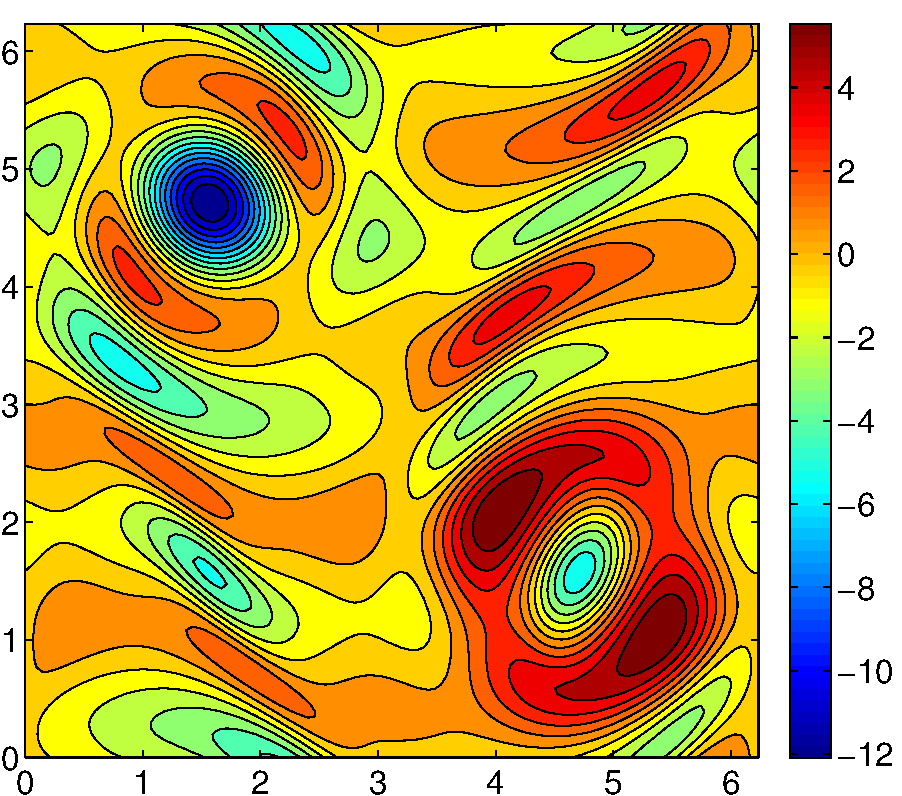
\includegraphics[width=.45\textwidth]{Kol_R40_n128_vort_adj+newton}
%	(b)\includegraphics[width=.45\textwidth]{Kol_R40_n128_vort_E2}\\
%	(c)\includegraphics[width=.45\textwidth]{Kol_R40_n128_vort_E2-1}
%	(d)\includegraphics[width=.45\textwidth]{Kol_R40_n128_vort_E3}
%	(e)\includegraphics[width=.45\textwidth]{Kol_R40_n128_vort_E2sin}
%	(f)\includegraphics[width=.45\textwidth]{Kol_R40_n128_vort_E4-1sin}
%	\caption{$Re=40$ and resolution $128^2$.
%		(a) Initial condition $\mathbf
%		u(x,y)=(2\cos(y),2\cos(x))$ converged with residue $5\times 10^{-13}$.
%		(b) Initial condition $\mathbf u(x,y)=(2\cos(2y),2\cos(2x))$ converged with
%		residue $1\times 10^{-13}$.
%		(c) Initial condition $\mathbf
%		u(x,y)=(2\cos(2y),2\cos(x))$ converged with residue $1\times 10^{-9}$
%		(d) Initial condition
%		$\mathbf u(x,y)=(2\cos(3y),2\cos(3x))$ converged with residue $4\times 10^{-13}$.
%		(e) Initial condition
%		$\mathbf u(x,y)=(\sin(2y),\sin(2x))$ converged with residue $4\times 10^{-9}$.
%		(f) Initial condition
%		$\mathbf u(x,y)=(0.5\sin(4y),3\sin(x))$ converged with residue $2\times 10^{-9}$.
%	}
%	
%	\label{fig:Kol_R40_E3}
%\end{figure}
%


%The understanding of chaotic dynamics in high-dimensional systems
%
%adjoint-based
%method to compute invariant solutions in partial differential equations.
%
%use 2 systems, Kuramoto-Sivashinsky equation and forced two-dimensional
%Navier-Stokes equation, to demonstrate the effectiveness of this new method.
%
%Correlations is all we know about high $Re$ Kolmogorov regime,
%but in the transitional regime everything is dominated by large coherent structures
%that as as non-statistical as can be. That's the whole point of the dynamical theory of
%turbulence; we know exact solutions in detail, no need to make statistical assumptions,
%look at averages that loose all interesting information.

%We start with the more accessible
%finite dimensional case (Section~\ref{sec:descend_fd}) that paves the way to the infinite
%dimensional case discussed in
%Section~\ref{sec:descend_inf}
%\subsection{Finite-dimensional case}\label{sec:descend_fd}
%Consider the differential equation
%\beq
%\frac{\mbox d\vc x}{\mbox d t} = \vc F(\vc x),
%\label{eq:ode}
%\eeq
%where $\vc x\in\mathbb R^n$ and $\vc F:\mathbb R^n\rightarrow\mathbb R^n$. Let
%$f^t:\mathbb R^n\rightarrow\mathbb R^n$ be the dynamical system generated by
%\eqref{eq:ode}. To determine the equilibria (or fixed points) of this dynamical system,
%one needs to solve the nonlinear system of equations
%\beq
%\vc F(\vc x) = 0.
%\eeq
%This is usually done by Newton iterations. While well-known, it is rarely mentioned that
%the Newton iterations are the explicit Euler step for a continuous-time differential
%equation.
%
%To see this, consider the problem of finding a one parameter family of group
%transformations $g^\tau:\mathbb R^n\to\mathbb R^n$ such that, for all $\vc x\in\mathbb
%R^n$,
%\beq
%\|\vc F(g^\tau (\vc x))\|^2\to 0, \quad \mbox{as} \quad t\to\infty,
%\label{eq:asymp_fd}
%\eeq
%where $\|\cdot\|$ is the Euclidean norm and the group parameter $\tau$ is a fictitious
%time. Designing $g^\tau$ such that \eqref{eq:asymp_fd} holds, the
%flow $g^\tau$ takes any initial condition
%$\vc x$ to a fixed point of the system \eqref{eq:ode} as `time' $\tau$ approaches
%infinity.
%
%Taking the derivative with respect to $\tau$, we have
%\beq
%\frac{\mbox d}{\mbox d\tau}\|\vc F(g^\tau (\vc x))\|^2=2\langle \bnabla\vc
%F(g^\tau(\vc x))\frac{\mbox d}{\mbox d \tau}g^\tau(\vc x),\vc F(g^\tau(\vc x))\rangle.
%\label{eq:dFdt}
%\eeq
%For \eqref{eq:asymp_fd} to hold, it is sufficient to require the right hand side of the
%above equation to be negative for all $\tau$. Hence we require that
%\beq
%\langle \bnabla \vc F(\vc x)\vc G(\vc x),\vc F(\vc x)\rangle <0,
%\label{eq:descendCond_fd}
%\eeq
%for all $\vc x\in\mathbb R^n$, where the vector filed $\vc G:\mathbb
%R^n\to\mathbb R^n$ is the generator of $g^\tau$, i.e.,
%\beq
%\frac{\mbox d\vc x}{\mbox d \tau}=\vc G(\vc x).
%\label{eq:ode_fict}
%\eeq
%An obvious choice for the the vector field $\vc G$ satisfying \eqref{eq:descendCond_fd} is
%\beq
%\frac{\mbox d\vc x}{\mbox d \tau}=\vc G(\vc x):=-\left[\bnabla\vc F(\vc x)\right]^{-1}\vc
%F(\vc x).
%\label{eq:Newton_dir}
%\eeq
%One can readily verify that with this choice of $\vc G$, the solutions of the
%differential equation \eqref{eq:ode_fict} converge to fixed points of $\vc F$ at an
%exponential rate. More specifically, due to identity \eqref{eq:dFdt}, we have
%$\|\vc F(g^\tau (\vc x))\|^2=\|\vc F(\vc x)\|^2\exp(-2\tau)$ for all $\tau>0$.
%The only way this convergence can fail is when the trajectory $g^\tau(\vc x)$
%approaches a singularity of $\bnabla\vc F$ where the vector field $\vc G$ is no longer
%defined.
%
%The Newton iteration,
%\beq
%\vc x_{i+1}=\vc x_i-\delta\tau\;\left[\bnabla\vc F(\vc x_i)\right]^{-1}\vc
%F(\vc x_i),
%\label{eq:newton_it}
%\eeq
%is the explicit Euler discretization of the differential equation \eqref{eq:Newton_dir},
%where $\delta\tau=1$ corresponds to the standard Newton iterations.
%
%Both continuous-time Newton descend~\eqref{eq:Newton_dir} and the discrete Newton
%iterations~\eqref{eq:newton_it} require the computation of the descend direction $\vc
%G(\vc x)=-\left[\bnabla\vc F(\vc x)\right]^{-1}\vc F(\vc x)$. For large systems, the
%matrix inversion $\left[\bnabla\vc F(\vc x)\right]^{-1}$ is computationally impractical.
%Instead, the descend direction is often approximated as the solution of the linear system
%$\bnabla\vc F(\vc x)\vc G(\vc x)=-\vc F(\vc x)$ through the generalized minimal residual
%(GMRES) algorithm. The resulting iterative method is often referred to as the
%Newton--GMRES algorithm. While significantly cheaper than matrix inversion, the
%Newton-GMRES algorithm is still computationally expensive for solving the
%differential equation \eqref{eq:Newton_dir}. As a result, the Newton iterations
%\eqref{eq:newton_it} are preferable. The drawback, however, is that the Newton-GMRES
%iterations are guaranteed to converge only when relatively accurate initial guesses are
%available.
%
%A computationally cheap alternative to the Newton descend is the adjoint descend.
%The adjoint descend is obtained by defining
%\beq
%\frac{\mbox d\vc x}{\mbox d \tau}=\vc G(\vc x):=-[\bnabla\vc F(\vc x)]^\dagger\vc F(\vc
%x),
%\label{eq:adjoint_dir}
%\eeq
%where $\dagger$ denotes matrix transposition. The norm of the nonlinear function $\vc F$
%along the trajectories $g^\tau(\vc x)$ of \eqref{eq:adjoint_dir} satisfies the identity
%\beq
%\frac{\mbox d}{\mbox d \tau}\|\vc F(g^\tau(\vc x))\|^2=-\|[\bnabla\vc F(g^\tau(\vc
%x))]^\dagger\vc
%F(g^\tau(\vc x))\|^2,
%\eeq
%ensuring that the norm $\|\vc F(g^\tau(\vc x))\|$ decays as the fictitious time $\tau$
%increases. Therefore, as $\tau\to\infty$, $g^\tau(\vc x)$ approaches a fixed point of
%\eqref{eq:ode}. The only way in which the adjoint descend may fail is that the trajectory
%$g^\tau(\vc x)$ approaches a point $\tilde{\vc x}$ where $[\bnabla\vc F(\tilde{\vc
%x})]^\dagger\vc F(\tilde{\vc x})=0$ while $\vc F(\tilde{\vc x})\neq 0$.
%
%As opposed to the Newton descend direction, computing the
%adjoint descend direction is cheap. Therefore, the differential equation
%\eqref{eq:adjoint_dir} may be solved numerically with more accurate numerical schemes
%than the first-order Euler step.



\section{Notes on Kolmogorov flow}
\label{s:KFlit}

\begin{description}
    \PCpost{2018-12-07}{
Moved the Mohammad / Predrag 2D Kolmogorov flow
discussions to svn repo \emph{siminos/spatiotemp/blog.tex},
which inputs \emph{chapter/Kolmogorov.tex}, with elton blog \emph{KFsymm.tex}
now input as section \emph{sect:KFsymm}
    }
\end{description}




\end{description}
